% !TeX spellcheck = de_DE


\chapter{Einleitung}
	Die Veranstaltung "Data Mining und Maschinelles Lernen" behandelt, ebenso wie diese Zusammenfassung, den Teilbereich des maschinellen Lernens der künstlichen Intelligenz. Dabei werden Algorithmen entwickelt, durch die ein Computer sich selbstständig verbessert. Ein Teilgebiet dieses maschinellen Lernens ist das \emph{tiefe Lernen} (DL, für \emph{Deep Learning}), bei dem tiefe künstliche neuronale Netzwerke genutzt werden (dies wird im \autoref{c:deepLearning} näher behandelt). Dieser Zusammenhang ist in \autoref{fig:aiMlDl} dargestellt.

	Diese Zusammenfassung wird in die folgenden Bereiche einführen: k-Nächste Nachbarn, Lineare Modelle und Funktionsapproximation, Modellselektion und Evaluierung, Entscheidungsbäume, Ensemble-Methoden, Naive Bayes und Bayes-Netzwerke, die Stützvektormethode, Clusteranalyse und Assoziationsregeln und (Tiefe) Neuronale Netzwerke. Viele andere Bereiche werden allerdings auch nicht abgedeckt, \bspw Variational Learning, Details des Deep Learning, Gaussian Processes, Graphische Modelle, Kausalität, \dots Diese Inhalte sind zu Teilen in den Zusammenfassungen für die Kurse "Statistical Machine Learning", "Probabilistic Graphical Models" (noch nicht verfügbar, voraussichtlich im Wintersemester 2021/22), "Statistical Relational AI" (noch nicht verfügbar, voraussichtlich im Wintersemester 2021/22) sowie "Deep Learning: Architectures and Methods" (bald verfügbar) zu finden.

	\begin{figure}
		\centering
		\begin{tikzpicture}[align = center]
			\node (dl) {Tiefes \\ Lernen};
			\node [right = 1 of dl] (ml) {Maschinelles \\ Lernen};
			\node [right = 1 of ml] (ai) {Künstliche Intelligenz};

			\path (dl) -- coordinate(needle) (ml);

			\node [draw, ellipse, minimum height = 1.5cm, minimum width = 2cm] at (dl) {};
			\node [draw, ellipse, minimum height = 3cm, minimum width = 7cm] at (needle) {};
			\node [draw, ellipse, minimum height = 5cm, minimum width = 13cm] at (ml) {};
		\end{tikzpicture}
		\caption{Zusammenhang von künstlicher Intelligenz, maschinellem Lernen und tiefem Lernen.}
		\label{fig:aiMlDl}
	\end{figure}

	\section{Geschichte}
		Im Gegensatz zu den meisten Vermutungen hat die künstliche Intelligenz bereits eine lange Vergangenheit:
		\begin{description}[leftmargin = 2cm]
			\item[1950er] Geburt der künstlichen Intelligenz
			\item[1960er] Ära der Perzeptrons
			\item[1970er] Erster KI-Winter
			\item[1980er] Ära der Expertensysteme
			\item[1990er] Zweiter KI-Winter
			\item[2000er] Ära des statistischen maschinellen Lernens
			\item[2000er] Ära des tiefen Lernens
		\end{description}
		Das Perzeptron, welches im folgenden Abschnitt vorgestellt wird, hat die ersten großen Ergebnisse in der KI-Forschung produziert. Es hat zwar eine sehr mächtige Vorhersagekraft, es gibt jedoch Probleme, die nicht mit einem Perzeptron lösbar sind (Minsky, 1969). Diese Tatsache hat anschließend zu dem ersten KI-Winter geführt, in dem wenig geforscht wurde und das öffentliche Interesse abgeebbt ist. Gefolgt ist die Ära der Expertensysteme, Fall- und Regal-basierte KI-Systeme, die durch einen Menschen und logisches Schlussfolgern erstellt wurden. Jedoch haben auch diese Systeme zu viel versprochen und das öffentliche Interesse ist schnell abgeebbt.

		Nun betrat das moderne maschinelle Lernen mit dem \emph{statistischen} maschinellen Lernen das Feld, welches durch komplizierte statistische Modelle angetrieben und motiviert wurde. Die Ergebnisse haben sehr viele Erfolge gebracht, es gab jedoch kein großes Pressecho. Dies könnte unter anderem daher kommen, dass der Grundsatz der Forschung quantitative und messbare Ergebnisse waren und keine großen Ansprüche zur "Intelligenz" gestellt wurden. Darauf folgte die Ära des tiefen Lernens, also neuronale Netzwerke mit "vielen" Schichten, welches ein große Aufmerksamkeit von der Presse und Politik bekommt.

		\subsection{Das Perzeptron}
			\label{subsec:perceptron}

			Das von Frank Rosenblatt entwickelte \emph{Perzeptron} war das erste Modell, welches durch das menschliche Gehirn motiviert war, ein künstliches neuronales Netzwerk. Dabei werden viele kleine und einfache Einheiten (Neuronen) zu einem größeren Modell verbunden und das Lernen findet durch Anpassung der Verbindungsstärken (Synapsen) und -gewichten statt. Eine Darstellung eines solchen Perzeptrons ist in \autoref{fig:perceptron} gegeben. Dabei werden die Eingaben in der Neuronenschicht gewichtet und die Neuronen \emph{feuern}. Diese Ausgabe wird anschließend an das Ausgabeneuron weitergegeben, welches die \emph{Aktivierungen} akkumuliert und, sofern der akkumulierte Wert über einen gewissen Schwellenwert liegt, feuert. So kann eine binäre Klassifikation durchgeführt werden.

			Zum trainieren eines Perzeptrons werden bekannte Daten verwendet, in das Perzeptron eingegeben und die vorhergesagten Ergebnisse mit den echten verglichen. War die Vorhersage korrekt, wird nicht geändert. War die Vorhersage jedoch falsch, so werden die Verbindungsstärken so geändert, dass das Richtige vorhergesagt wird. Dies wird so lange wiederholt, bis keine Fehler mehr gemacht werden.

			Mit dem Wechsel zu tiefem Lernen werden diese einschichtigen nicht mehr verwendet, sondern es werden mehrere Neuronenschichten verwendet, die aufeinander Aufbauen (in \autoref{fig:mlp} in ein solches Netzwerk gezeigt). Neben der Nachteile des höheren Speicherverbrauchs, mehr benötigter Rechenkraft und der Anforderung an mehr Daten haben solche Modelle den großen Vorteil, dass sie eine deutlich höhere Vorhersagekraft besitzen.

			\begin{figure}
				\centering
				\begin{tikzpicture}[->]
					\node [input neuron] (a) {};
					\node [input neuron, below = 0.1 of a] (b) {};
					\node [input neuron, below = 0.1 of b] (c) {};
					\node [input neuron, below = 0.1 of c] (d) {};
					\node [input neuron, below = 0.1 of d] (e) {};

					\node [left = 2 of c] (I) {Input};

					\node [output neuron, right = 2 of c] (o) {};
					\node [right = 1 of o] (O) {Output};

					\draw (a) to[bend left = 10] (o);
					\draw (b) to[bend left = 5] (o);
					\draw (c) to (o);
					\draw (d) to[bend right = 5] (o);
					\draw (e) to[bend right = 10] (o);

					\draw (I) to[bend left = 10] (a);
					\draw (I) to[bend left = 5] (b);
					\draw (I) to (c);
					\draw (I) to[bend right = 5] (d);
					\draw (I) to[bend right = 10] (e);

					\draw (o) to (O);
				\end{tikzpicture}
				\caption{Darstellung eines einschichtigen Perzeptrons.}
				\label{fig:perceptron}
			\end{figure}

			\begin{figure}
				\centering
				\begin{tikzpicture}
					\node [input neuron] (a) {};
					\node [input neuron, below = 0.1 of a] (b) {};
					\node [input neuron, below = 0.1 of b] (c) {};
					\node [input neuron, below = 0.1 of c] (d) {};
					\node [input neuron, below = 0.1 of d] (e) {};

					\node [neuron, right = 1.5 of a] (l11) {};
					\node [neuron, right = 1.5 of b] (l12) {};
					\node [neuron, right = 1.5 of c] (l13) {};
					\node [neuron, right = 1.5 of d] (l14) {};
					\node [neuron, right = 1.5 of e] (l15) {};

					\node [neuron, right = 1.5 of l11] (l21) {};
					\node [neuron, right = 1.5 of l12] (l22) {};
					\node [neuron, right = 1.5 of l13] (l23) {};
					\node [neuron, right = 1.5 of l14] (l24) {};
					\node [neuron, right = 1.5 of l15] (l25) {};

					\node [neuron, right = 1.5 of l21] (l31) {};
					\node [neuron, right = 1.5 of l22] (l32) {};
					\node [neuron, right = 1.5 of l23] (l33) {};
					\node [neuron, right = 1.5 of l24] (l34) {};
					\node [neuron, right = 1.5 of l25] (l35) {};

					\node [output neuron, right = 1 of l33] (o) {};

					\draw (l31) to (o);
					\draw (l32) to (o);
					\draw (l33) to (o);
					\draw (l34) to (o);
					\draw (l35) to (o);

					\draw (a) to (l11);
					\draw (a) to (l12);
					\draw (a) to (l13);
					\draw (a) to (l14);
					\draw (a) to (l15);
					\draw (b) to (l11);
					\draw (b) to (l12);
					\draw (b) to (l13);
					\draw (b) to (l14);
					\draw (b) to (l15);
					\draw (c) to (l11);
					\draw (c) to (l12);
					\draw (c) to (l13);
					\draw (c) to (l14);
					\draw (c) to (l15);
					\draw (d) to (l11);
					\draw (d) to (l12);
					\draw (d) to (l13);
					\draw (d) to (l14);
					\draw (d) to (l15);
					\draw (e) to (l11);
					\draw (e) to (l12);
					\draw (e) to (l13);
					\draw (e) to (l14);
					\draw (e) to (l15);

					\draw (l11) to (l21);
					\draw (l11) to (l22);
					\draw (l11) to (l23);
					\draw (l11) to (l24);
					\draw (l11) to (l25);
					\draw (l12) to (l21);
					\draw (l12) to (l22);
					\draw (l12) to (l23);
					\draw (l12) to (l24);
					\draw (l12) to (l25);
					\draw (l13) to (l21);
					\draw (l13) to (l22);
					\draw (l13) to (l23);
					\draw (l13) to (l24);
					\draw (l13) to (l25);
					\draw (l14) to (l21);
					\draw (l14) to (l22);
					\draw (l14) to (l23);
					\draw (l14) to (l24);
					\draw (l14) to (l25);
					\draw (l15) to (l21);
					\draw (l15) to (l22);
					\draw (l15) to (l23);
					\draw (l15) to (l24);
					\draw (l15) to (l25);

					\draw (l21) to (l31);
					\draw (l21) to (l32);
					\draw (l21) to (l33);
					\draw (l21) to (l34);
					\draw (l21) to (l35);
					\draw (l22) to (l31);
					\draw (l22) to (l32);
					\draw (l22) to (l33);
					\draw (l22) to (l34);
					\draw (l22) to (l35);
					\draw (l23) to (l31);
					\draw (l23) to (l32);
					\draw (l23) to (l33);
					\draw (l23) to (l34);
					\draw (l23) to (l35);
					\draw (l24) to (l31);
					\draw (l24) to (l32);
					\draw (l24) to (l33);
					\draw (l24) to (l34);
					\draw (l24) to (l35);
					\draw (l25) to (l31);
					\draw (l25) to (l32);
					\draw (l25) to (l33);
					\draw (l25) to (l34);
					\draw (l25) to (l35);
				\end{tikzpicture}
				\caption{Darstellung eines mehrschichtigen Perzeptrons.}
				\label{fig:mlp}
			\end{figure}
		% end
	% end

	\section{KI Heute}
		Heute gibt es vier entscheidende Unterschiede zu vergangenen KI-Systemen:
		\begin{enumerate}
			\item Die Modelle sind größer.
				\begin{itemize}
					\item Früher wurden neuronale Netzwerke mit ein bis drei Schichten und hunderte bis tausende Neuronen verwendet.
					\item Heutige Modelle haben hunderte Schichten und hunderttausende Neuronen.
				\end{itemize}
			\item Es sind mehr Daten verfügbar.
				\begin{itemize}
					\item Früher waren tausende Bilder, hunderte Stunden Audiomaterial und hunderttausende Wörter verfügbar.
					\item Heute sind es Milliarden Bilder, Milliarden Stunden Audiomaterial und hunderte Milliarden Wörter.
					\item Diese Daten werden dabei in vielen großen Firmen gesammelt, \bspw hat YouTube mehr als zehn Milliarden Videos, Alibaba tätigt mehr als zwölf Milliarden Verkäufe pro Jahr, Facebook-Nutzer laden hunderte Milliarden Bilder pro Jahr hoch und Google kennt mehr als hundert Billionen Webseiten.
				\end{itemize}
			\item Heute Computer sind Leistungsfähiger.
				\begin{itemize}
					\item Früher konnte eine CPU \ca eine Millionen Operationen pro Sekunde ausführen und es gab keine GPUs.
					\item Heutige CPUs können mehr als eine Billionen Operationen pro Sekunde und heutige GPUs können mehr als zehn Billionen Operationen pro Sekunde ausführen.
				\end{itemize}
			\item Die Systeme funktionieren und lösen viele Aufgaben.
		\end{enumerate}
		Dabei ist der Hauptmotor der künstlichen Intelligenz aktuell das maschinelle Lernen.
	% end

	\section{Was ist Maschinelles Lernen?}
		\emph{Maschinelles Lernen} ist die Automatisierung von Automatisierung, es werden Teile des Computers so programmiert, dass sie sich anschließend selbstständig "programmieren". Das ist nötig, da das Schreiben von Software oftmals der Flaschenhals in der Entwicklung ist, da die Daten so schnell mehr werden. Es ist also klug, die Daten zu nutzen, um die Software selbst zu erstellen. Im Gegensatz zur traditionellen Programmierung werden also keine Ausgaben durch ein Programm erstellt, sondern es wird ein Programm aus Ausgaben erstellen (siehe \autoref{fig:traditionalVsMl}). Die Entwicklung von ML-Komponenten ist dabei ein Kreislauf, dargestellt in \autoref{fig:mlPipeline}.

		Anwendungsgebiete von maschinellem Lernen sind beispielsweise Websuche, Computational Biologie/Cognitive Science/Social Science/\dots, Finanzwelt, E-Commerce, Robotik, Debugging, Industrie 4.0 und viele mehr.

		\begin{figure}
			\centering
			\begin{subfigure}{0.49\linewidth}
				\centering
				\begin{tikzpicture}
					\node [draw, rectangle, minimum height = 1cm, minimum width = 2.5cm] (a) {Computer};
					\coordinate [above = 0.3 of a.west] (b);
					\coordinate [below = 0.3 of a.west] (c);
					\node [left = 0.75 of b] (d) {Daten};
					\node [left = 0.75 of c] (e) {Programm};
					\node [right = 0.75 of a.east] (f) {Ausgabe};
					\draw [->] (d) to (b);
					\draw [->] (e) to (c);
					\draw [->] (a.east) to (f);
				\end{tikzpicture}
				\caption{Traditionelle Programmierung}
			\end{subfigure}
			~
			\begin{subfigure}{0.49\linewidth}
				\centering
				\begin{tikzpicture}
					\node [draw, rectangle, minimum height = 1cm, minimum width = 2.5cm] (a) {Computer};
					\coordinate [above = 0.3 of a.west] (b);
					\coordinate [below = 0.3 of a.west] (c);
					\node [left = 0.75 of b] (d) {Daten};
					\node [left = 0.75 of c] (e) {Ausgabe};
					\node [right = 0.75 of a.east] (f) {Programm};
					\draw [->] (d) to (b);
					\draw [->] (e) to (c);
					\draw [->] (a.east) to (f);
				\end{tikzpicture}
				\caption{Maschinelles Lernen}
			\end{subfigure}
			\caption{Traditionelle Programmierung (links) im Vergleich zu maschinellem Lernen (rechts).}
			\label{fig:traditionalVsMl}
		\end{figure}

		\begin{figure}
			\centering
			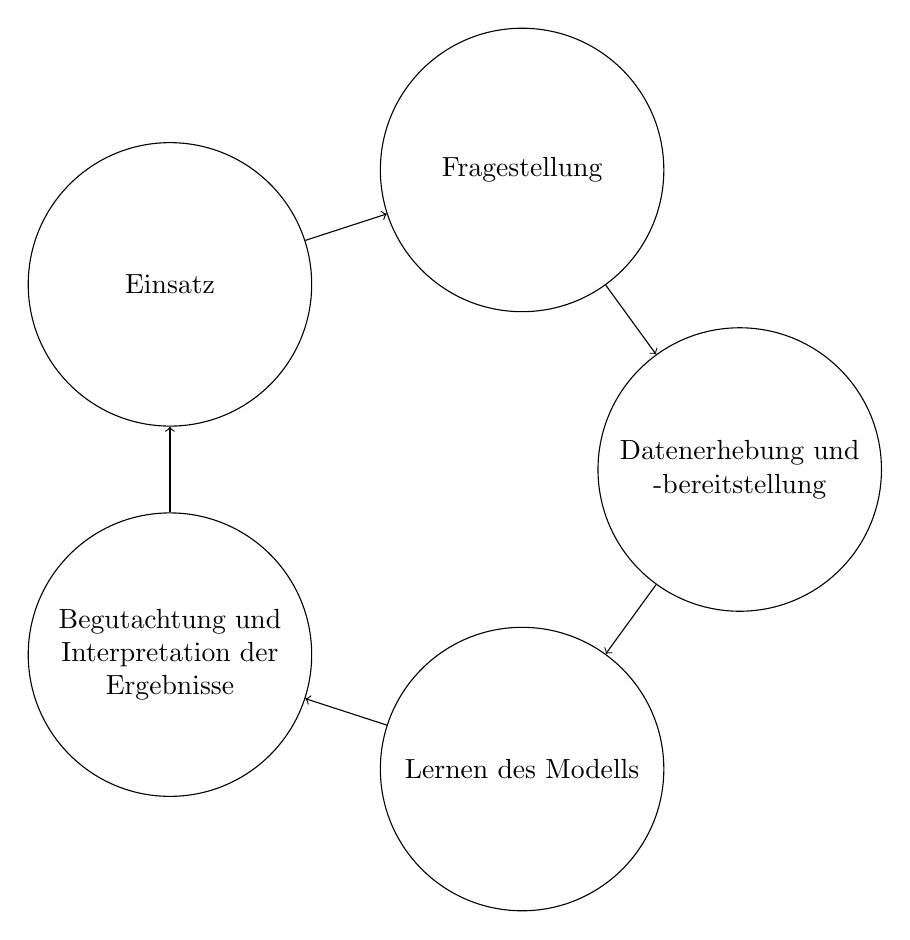
\begin{tikzpicture}[->, align = center, every node/.style = { draw, circle, minimum height = 2cm, minimum width = 3.6cm }]
				\node (a) at (-288:4cm) {Fragestellung};
				\node (b) at (-  0:4cm) {Datenerhebung und \\ -bereitstellung};
				\node (c) at (- 72:4cm) {Lernen des Modells};
				\node (d) at (-144:4cm) {Begutachtung und \\ Interpretation der \\ Ergebnisse};
				\node (e) at (-216:4cm) {Einsatz};
				\draw (a) to (b);
				\draw (b) to (c);
				\draw (c) to (d);
				\draw (d) to (e);
				\draw (e) to (a);
			\end{tikzpicture}
			\caption{Kreislauf der Erstellung von ML-Komponenten.}
			\label{fig:mlPipeline}
		\end{figure}

		\subsection{Kurzgefasst}
			Im Bereich des maschinellen Lernens gibt es viele tausende Algorithmen und hunderte neue Algorithmen pro Jahr. Dabei adressiert jeder Algorithmus die folgenden drei Fragestellungen:
			\begin{enumerate}
				\item Wie wird das Modell \emph{repräsentiert}? \\
					Entscheidungsbäume, Regeln/logische Programme, Instanzen, Probabilistische Graphische Modelle, Neuronale Netzwerke, Stützvektormaschinen, Ensembles, \dots
				\item Wie wird das Modell \emph{optimiert}? \\
					Kombinatorische Optimierung (\zB Greedy-Suche), Konvexe und nichtlineare Optimierung (\zB Gradientenabstieg), Optimierung unter Randbedingungen (\zB lineare Programmierung), \dots
				\item Wie wird das Modell \emph{evaluiert} und \emph{beurteilt}? \\
					Korrektklassifikationsrate (Accuracy), Genauigkeit (Precision) und Trefferquote (Recall), Quadrierter Fehler, Likelihood, A-Posteriori Wahrscheinlichkeit, Kosten/Nutzen, Margin, Entropie, KL-Divergenz, \dots
			\end{enumerate}

			Dabei gibt es vier große Kategorien des maschinellen Lernens:
			\begin{description}
				\item[Überwacht (Induktiv)] Die Trainingsdaten erhalten neben Eingaben auch gewünschten Ausgaben. \\
					Englisch: \emph{Supervised Learning}
				\item[Unüberwacht] Die Trainingsdaten erhalten nur Eingaben und \emph{keine} Ausgaben. \\
					Englisch: \emph{Unsupervised Learning}
				\item[Teilweise Überwacht] Die Trainingsdaten \emph{einige} gewünschte Ausgaben, aber nicht alle. \\
					Englisch: \emph{Semi-supervised Learning}
				\item[Verstärkend] Der Algorithmus wird belohnt nachdem er eine Reihe an Aktionen ausgeführt hat und die Belohnung wird maximiert. \\
					Englisch: \emph{Reinforcement Learning}
			\end{description}
			Die Bereiche des überwachten und unüberwachten Lernens lassen sich dann noch weiter einordnen, was in \autoref{fig:mlTypes} gezeigt ist.

			\begin{figure}
				\centering
				\begin{tikzpicture}[
							->,
							align = center,
							block/.style = {
								draw,
								rectangle,
								minimum width = 3.25cm,
								minimum height = 1.5cm,
							},
								small/.style = {
								minimum height = 0.8cm,
							},
						]
					\node [block] (ml) {Maschinelles \\ Lernen};
					\node [block, right = 2 of ml, yshift = +3cm] (supervised) {Überwachtes \\ Lernen};
					\node [block, right = 2 of ml] (unsupervised) {Unüberwachtes \\ Lernen};
					\node [block, right = 2 of ml, yshift = -3cm] (rl) {Verstärkendes \\ Lernen};

					\node [block, small, right = 2 of supervised, yshift = +0.75cm] (class) {Klassifikation};
					\node [block, small, right = 2 of supervised, yshift = -0.75cm] (regress) {Regression};

					\node [block, small, right = 2 of unsupervised, yshift = +0.75cm] (dimred) {Dim.-Reduktion};
					\node [block, small, right = 2 of unsupervised, yshift = -0.75cm] (cluster) {Clustering};

					\draw (ml.east) to [bend right, out = -45+10, in = +180-45] (supervised.west);
					\draw (ml.east) to (unsupervised.west);
					\draw (ml.east) to [bend left,  out = +45-10, in = -180+45] (rl.west);

					\draw (supervised.east) to [bend right, out = -45+30, in = +180-45+30] (class.west);
					\draw (supervised.east) to [bend left,  out = +45-30, in = -180+45-30] (regress.west);

					\draw (unsupervised.east) to [bend right, out = -45+30, in = +180-45+30] (dimred.west);
					\draw (unsupervised.east) to [bend left,  out = +45-30, in = -180+45-30] (cluster.west);
				\end{tikzpicture}
				\caption{Arten des maschinellen Lernens.}
				\label{fig:mlTypes}
			\end{figure}
		% end
	% end
% end

\chapter{Grundlagen}
	Dieses Kapitel behandelt einige Grundlagen, die für das maschinelle Lernen benötigt werden.

	\section{CRISP-DM: Verlaufsmodell des Data Mining}
		Die Schritte des CRISP-DM (Cross-Industry Standard Process for Data Mining), dem Verlaufsmodell des Data Mining, sind:
		\begin{description}
			\item[Problem Verstehen] Analyseziele, Situationsbewertung, Datenanalyseziele, Projektplan
			\item[Daten Verstehen] Sammeln, Beschreiben, Untersuchen, Qualität von Rohdaten
			\item[Daten Aufbereiten] Ein- und Ausschluss, Bereinigung, Transformation von Variablen
			\item[Modellierung] Methoden- und Testdesignwahl, Schätzung, Modellqualität
			\item[Evaluierung] Modell akzeptieren, Prozess überprüfen, Nächste Schritte festlegen
			\item[Nachbereitung] Anwendungs- und Wartungsplan, Präsentation, Bericht
		\end{description}
		Diese Schritte sind grafisch in \autoref{fig:crisp} dargestellt.

		\begin{figure}
			\centering
			\includegraphics[width=0.5\linewidth]{img/crisp-dm}
			\caption{Grafische Übersicht über das CRISP-DM. \\ Autor: Kenneth Jensen \\ Lizenz: CC BY-SA 3.0 \\ Quelle: Wikipedia Commons, Datei CRISP-DM\_Process\_Diagram.png}
			\label{fig:crisp}
		\end{figure}
	% end

	\section{Klassifikation und Regression}
		Bei überwachtem maschinellen Lernen wird jeder Beobachtung \(\vec{x}\) ein Label \(y\) zugeordnet, \dh die Datenpunkte sind gegeben als \( (\vec{x}, y) \in X \times Y \), wobei \(X\) und \(Y\) die Mengen aller möglichen Beobachtungen/Labels sind. Im Teilbereich der \emph{Klassifikation} sind die Labels diskret, \dh es wird eine \emph{qualitative} Beschreibung gesucht. Im Gegensatz dazu steht die \emph{Regression}, bei der die Labels kontinuierlich sind und eine \emph{quantitative} Beschreibung gesucht wird.

		Das Ziel ist immer eine \emph{wahre Funktion} \( f : X \to Y \) zu finden, die für alle Eingaben \( \vec{x} \in X \) und Labels \( y \in Y \) den korrekten Wert liefert, \dh \( f(\vec{x}) = y \). Das Problem ist im Allgemeinen, dass nur eine Teilmenge aller Beobachtungen gegeben ist, die \emph{Trainingsdaten}. Auf Basis dieser Trainingsdaten wird nun eine Annäherung \( \hat{f} \) an die wahre Funktion \(f\) gesucht, welche als \emph{Modell} bezeichnet wird. Wurde ein Modell gefunden, so liefert dieses über
		\begin{equation}
			\hat{y} = \hat{f}(\vec{x})
		\end{equation}
		eine \emph{Vorhersage} \( \hat{y} \in Y \) für ein Datum \( \vec{x} \in X \).

		Dabei kann zur Klassifikation sowohl ein spezifisches als auch ein Regressionsmodell genutzt werden. Es können zum Beispiel alle Werte oberhalb eines Schwellenwertes \(\theta\) der einen und alle anderen Werte der anderen Klasse (im Fall von binären Klassifikationsproblemen) zugeordnet werden:
		\begin{equation}
			\hat{y} =
				\begin{cases}
					+1 & \text{falls } \hat{f}(\vec{x}) \geq \theta \\
					-1 & \text{sonst}
				\end{cases}
		\end{equation}
		Diese Art der Zuordnung ist nur eine Möglichkeit, ein Regressionsmodell als Klassifikationsmodell zu nutzen. Eine weitere ist \zB die logistische Regression, siehe \autoref{sec:logisticRegression}.
	% end

	\section{Statistik}
		In diesem Abschnitt werden benötigte grundlegenden Begriffe der Statistik eingeführt.

		\subsection{Erwartungswert, Varianz und Standardabweichung}
			Für eine diskrete Zufallsvariable \(X\) mit Werten \( x_i \) ist der \emph{Erwartungswert} gegeben durch
			\begin{equation}
				\E[X] = \sum_i x_i P(X = x_i).
			\end{equation}
			Für eine kontinuierliche Zufallsvariable \(X\) mit der Wahrscheinlichkeitsdichte \(p\) wird die Summe durch ein Integral ersetzt:
			\begin{equation}
				\E[X] = \int_{-\infty}^{\infty} \! x f(x) \dd{x}
			\end{equation}
			Oftmals werden dabei die Integrationsgrenzen weggelassen.

			Eine wichtige Eigenschaft des Erwartungswerts ist, dass dieser linear ist, \dh es gilt
			\begin{equation}
				\E[aX + bY] = a \E[X] + b \E[Y]
			\end{equation}
			für zwei Zufallsvariablen \(X\), \(Y\) und skalare \(a\), \(b\). Sind die Zufallsvariablen \(X\), \(Y\) stochastisch unabhängig, so gilt
			\begin{equation}
				\E[XY] = \E[X] \E[Y]
			\end{equation}

			Die \emph{Varianz} einer Zufallsvariablen ist gegeben durch die mittlere quadratische Abweichung vom Mittelwert,
			\begin{equation}
				\Var[X] = \E\big[ (X - \E[X])^2 \big].
			\end{equation}
			Sie wird oft auch mit \(\sigma^2\) bezeichnet. Die \emph{Standardabweichung} einer Zufallsvariable ist dann \(\sigma = \sqrt{\Var[X]}\). Nach dem \emph{Verschiebungssatz} gilt, wie einfach herzuleiten ist:
			\begin{equation}
				\Var[X] = \E\big[ (X - \E[X])^2 \big] = \E\big[ X^2 \big] - \big( \E[X] \big)^2.
			\end{equation}
		% end

		\subsection{Bias}
			\label{subsec:foundationsBias}

			Der \emph{Bias} eines Schätzers \(\hat{y}\) für eine Zufallsvariable \(Y\) bezeichnet die mittlere Verzerrung
			\begin{equation}
				\Bias[\hat{y}] = \E[Y - \hat{y}] = \E[Y] - \hat{y}
			\end{equation}
			des Schätzers. Ein Schätzer mit einem Bias von Null wird als \emph{Erwartungstreu} oder \emph{Unbiased} bezeichnet.

			Oftmals kann bei einem Schätzer nur entweder die Varianz oder der Bias reduziert werden, was als \emph{Bias-Varianz Trade-Off} bezeichnet wird.
		% end

		\subsection{Normalverteilung}
			Die \emph{Normalverteilung} (auch \emph{Gauß-Verteilung}) ist eine der wichtigsten Wahrscheinlichkeitsverteilungen in der Statistik. Dabei heißt eine Zufallsvariable \(X\) \emph{normalverteilt} mit Mittelwert \(\mu\) und Varianz \(\sigma^2\), wenn sie die Wahrscheinlichkeitsdichte
			\begin{equation}
				p(x) = \frac{1}{\sqrt{2 \pi \sigma^2}} \exp\bigg\{\!\! -\frac{1}{2} \frac{(x - \mu)^2}{\sigma^2} \bigg\}
			\end{equation}
			besitzt.
		% end

		\subsection{Bedingte Wahrscheinlichkeiten}
			Bedingte Wahrscheinlichkeiten, geschrieben \( P(X = x \given Y = y) \), beschreiben die Wahrscheinlichkeit einer Zufallsvariable \(X\) den Wert \(x\) anzunehmen, wenn eine andere Zufallsvariable \(Y\) den Wert \(y\) hat. Zufallsvariablen \(X\), \(Y\) heißen \emph{stochastisch unabhängig}, wenn \( P(X = x \given Y = y) = P(X = x) \) gilt. Im Allgemeinen gilt
			\begin{equation}
				P(X \given Y = y) = \frac{P(X = x, Y = y)}{P(Y = y)},
			\end{equation}
			wobei \( P(X = x, Y = y) \) die \emph{Verbundwahrscheinlichkeit} ist.
		% end

		\subsection{Bayes-Statistik}
			Eine der wichtigsten Formeln in der Statistik in die Bayes-Formel
			\begin{equation}
				p(x \given y) = \frac{p(y \given x) \, p(x)}{p(y)},
			\end{equation}
			die den Zusammenhang zwischen der Likelihood \( p(y \given x) \), der A-Priori Wahrscheinlichkeit \( p(x) \) und der A-Posteriori Wahrscheinlichkeit \( p(x \given y) \) beschreibt. Der Faktor \( p(y) \) dient dabei nur der Normalisierung, weshalb die Bayes-Formel oft auch als
			\begin{equation}
				p(x \given y) \propto p(y \given x) \, p(x)
			\end{equation}
			geschrieben wird.
		% end

		\subsection{Konfidenzintervalle}
			Ein \emph{Konfidenzintervall} ist ein Intervall \( [\ell, u] \), welches aus einer gegebenen Irrtumswahrscheinlichkeit \(\alpha\) erzeugt wird. Es gibt den Bereich an, in dem der Wert der Zufallsvariable mit Wahrscheinlichkeit \( 1 - \alpha \) liegt:
			\begin{equation}
				P(\ell \leq X \leq u) = 1 - \alpha
			\end{equation}
			Eine häufige Wahl ist die Bildung eines Konfidenzintervalls für den Erwartungswert. So können Aussagen wie "Mit \SI{99}{\percent} Wahrscheinlichkeit liegt der Mittelwert im Intervall \( [\ell, u] \)." getätigt werden (hier mit \( \alpha = 0.01 \)).

			Konfidenzintervalle sind ein mächtiges Werkzeug in der Bewertung von Verfahren, was in \autoref{c:trees} weiter behandelt wird.
		% end

		\subsection{Entropie}
			Die Entropie einer Wahrscheinlichkeitsverteilung \(P(X)\) gibt an, wie viel Informationsgehalt in dieser steckt. Für eine diskrete Zufallsvariable \(X\) mit den möglichen Werten \(\mathcal{X}\) wird die Entropie wie folgt berechnet:
			\begin{equation}
				H(X) = -\!\sum_{x \,\in\, \mathcal{X}} P(x) \,\log P(x)
			\end{equation}
			Für eine kontinuierliche Zufallsvariable \(X\) mit Wahrscheinlichkeitsdichte \(p(X)\) gilt
			\begin{equation}
				H(X) = -\!\int\! p(x) \,\log p(x) \dd{x}\!,
			\end{equation}
			wobei wie vorher beschrieben die Integrationsgrenzen zur Übersichtlichkeit weggelassen werden. Wird der Logarithmus zur Basis \num{2} verwendet, so kann die Entropie einer Verteilung auch als die Anzahl Bits angesehen werden, die mindestens zur Übertragung benötigt werden.

			\subparagraph{Beispiel}
				Es werden Nachrichten \(X\) mit den Werten \(a\), \(b\), \(c\) und \(d\) versendet. Eine Aufzeichnung des Netzwerkverlaufs stellt fest, dass die Nachrichten mit den folgenden Häufigkeiten gesendet werden:
				\begin{center}
					\begin{tabular}{c|c|c|c}
						\(a\) & \(b\) & \(c\) & \(d\) \\ \hline
						 25   &   7   &  14   &  54
					\end{tabular}
				\end{center}
				Bei einer Gesamtanzahl von \( 25 + 7 + 14 + 54 = 100 \) ergeben sich also die folgenden relativen Häufigkeiten, \bzw die folgende empirische Verteilung:
				\begin{equation}
					\begin{aligned}
						P(X = a) &= 25\% &
						P(X = b) &= 7\%  \\
						P(X = c) &= 14\% &
						P(X = d) &= 54\%
					\end{aligned}
				\end{equation}
				Der Informationsgehalt \( -\log_2 P(X) \) je Symbol ist:
				\begin{equation}
					\begin{aligned}
						-\log_2 P(X = a) &= 2      &
						-\log_2 P(X = b) &= 3.8365 \\
						-\log_2 P(X = c) &= 2.8365 &
						-\log_2 P(X = d) &= 0.888969
					\end{aligned}  \label{eq:entropyExampleInformation}
				\end{equation}
				Daraus ergibt sich die folgende Gesamtentropie:
				\begin{align}
					H(X)
						&= -\big(
								\begin{aligned}[t]
									 &\, \eqmakebox[entropyExample][l]{\(\displaystyle P(X = a)\)} \,\log P(X = a) \\
								   + &\, \eqmakebox[entropyExample][l]{\(\displaystyle P(X = b)\)} \,\log P(X = b) \\
								   + &\, \eqmakebox[entropyExample][l]{\(\displaystyle P(X = c)\)} \,\log P(X = c) \\
								   + &\, \eqmakebox[entropyExample][l]{\(\displaystyle P(X = d)\)} \,\log P(X = d) \quad\big)
								\end{aligned}
						\\
						&= 0.25 \cdot 2 + 0.007 \cdot 3.8365 + 0.14 \cdot 2.8365 + 0.54 \cdot 0.888969 \\
						&= 1.40401
				\end{align}
				Es werden also mindestens \num{2} Bits benötigt, um die Nachricht zu kodieren.

				An dem Informationsgehalt \eqref{eq:entropyExampleInformation} ist zu sehen, dass as Symbol \(d\) die wenigsten Informationen überträgt, da es am häufigsten vorkommt. Dies kann Interpretiert werden als "Überraschungseffekt" beim Empfänger: Kommt ein \(d\) an, ist dies nicht überraschen, da dies in \SI{54}{\%} der Fälle passiert. Kommt jedoch ein \(b\) an, ist dies sehr ungewöhnlich.
			% end
		% end
	% end
% end

\chapter{k-Nächste Nachbarn (kNN)}
	Im Allgemeinen können Verfahren des maschinellen Lernens in \emph{globale} und \emph{lokale} Modelle unterteilt werden: Lokale Modelle Klassifizieren einen Datenpunkt nur Anhand seiner Umgebung, globale Modelle hingegen finden ein global Gültiges Entscheidungskriterium, beispielsweise eine trennende Hyperebene. Das verfahren der \emph{k-Nächsten Nachbarn} (kNN) gehört zu den lokalen Modelle. Bei diesem Ansatz wird ein Beispiel anhand der \(k\) nächsten Nachbarn (nach irgendeiner Ähnlichkeitsmetrik) klassifiziert: Ein Datenpunkt gehört einer bestimmten Klasse an, wenn der Großteil der umliegenden Datenpunkte auch dieser Klasse angehören. Leicht formalisiert ergibt sich folgendes Vorgehen (wobei \( f(\cdot) \) die tatsächliche Kategorie beschreibt):
	\begin{enumerate}
		\item Berechne den Abstand zwischen dem Datenpunkt \( \vec{x}_\ast \) und jedem Trainingsdatenpunkt.
		\item Wähle die \(k\) nächsten Nachbarn \( \dotsrange{\vec{n}_1}{\vec{n}_k} \) bezüglich einem Ähnlichkeitsmaß \( \mathit{dist}(\vec{x}, \vec{y}) \).
		\item Berechne die Vorhersage \( A\big( \vec{x}_\ast;\, \dotsrange{f(\vec{n}_1)}{f(\vec{n}_k)} \big) \).
	\end{enumerate}
	Hier werden sofort einige Schwierigkeiten ersichtlich:
	\begin{itemize}
		\item Welches Ähnlichkeitsmaß \( \mathit{dist}(\cdot, \cdot) \) sollte verwendet werden?
		\item Wie viele Nachbarn \(k\) sollten verwendet werden?
		\item Was passiert, wenn die Werte der Nachbarn nicht überein stimmen oder es ein Unentschieden gibt?
		\item Wie kann die Suche effizient gestaltet werden?
	\end{itemize}

	\section{Ähnlichkeitsmaße}
		Wie bereits beschrieben ist ein Problem die Auswahl eines Ähnlichkeitsmaßes. Die zwei wichtigsten Eigenschaften des Ähnlichkeitsmaßes sind, dass dieses kleiner werden sollte, wenn zwei Datenpunkte sich ähnlicher sind und genau dann Null ist, wenn zwei Datenpunkte identisch sind. Eine Möglichkeit ist beispielsweise der euklidische Abstand
		\begin{equation}
			\mathit{dist}(\vec{x}, \vec{y}) = \lVert \vec{x} - \vec{y} \rVert_2 = \sqrt{\textstyle \sum_{i = 1}^{n} (x_i - y_i)^2}
		\end{equation}
		oder der Kosinus-Abstand
		\begin{equation}
			\mathit{dist}(\vec{x}, \vec{y}) = \cos(\vec{x}, \vec{y}) = \frac{\braket{\vec{x}}{\vec{y}}}{\lvert \vec{x} \rvert \, \lvert \vec{y} \rvert} = \frac{\sum_{i = 1}^{n} x_i y_i}{\sqrt{\sum_{i = 1}^{n} x_i^2} \, \sqrt{\sum_{i = 1}^{n} y_i^2}},
		\end{equation}
		welcher Invariant gegenüber Skalierungen der Vektoren ist. Andere Ähnlichkeitsmaße für binäre (0/1) Daten sind \zB:
		\begin{itemize}
			\item Matching Koeffizient:
		\end{itemize}
		\begin{equation}
			\lvert \vec{x} \cap \vec{y} \rvert
		\end{equation}
		\begin{itemize}
			\item Dice Koeffizient:
		\end{itemize}
		\begin{equation}
			\frac{2 \lvert \vec{x} \cap \vec{y} \rvert}{\lvert \vec{x} \rvert + \lvert \vec{y} \rvert}
		\end{equation}
		\begin{itemize}
			\item Jaccard Koeffizient.
		\end{itemize}
		\begin{equation}
			\frac{\lvert \vec{x} \cap \vec{y} \rvert}{\lvert \vec{x} \cup \vec{y} \rvert}
		\end{equation}
		\begin{itemize}
			\item Overlap Koeffizient:
		\end{itemize}
		\begin{equation}
			\frac{\lvert \vec{x} \cap \vec{y} \rvert}{\min \{ \lvert \vec{x} \rvert, \lvert \vec{y} \rvert \}}
		\end{equation}
		\begin{itemize}
			\item Kosinus:
		\end{itemize}
		\begin{equation}
			\frac{\lvert \vec{x} \cap \vec{y} \rvert}{\sqrt{\lvert \vec{x} \rvert} \, \sqrt{\lvert \vec{y} \rvert}}
		\end{equation}
		Dabei beschreibt \( \cap \) eine komponentenweise Und-Aggregation und \( \cup \) eine Oder-Aggregation:
		\begin{align}
			\begin{bmatrix}
				0 \\ 0 \\ 1 \\ 1
			\end{bmatrix}
			\cap
			\begin{bmatrix}
				0 \\ 1 \\ 0 \\ 1
			\end{bmatrix}
			&=
			\begin{bmatrix}
				0 \\ 0 \\ 0 \\ 1
			\end{bmatrix}
			&
			\begin{bmatrix}
				0 \\ 0 \\ 1 \\ 1
			\end{bmatrix}
			\cup
			\begin{bmatrix}
				0 \\ 1 \\ 0 \\ 1
			\end{bmatrix}
			&=
			\begin{bmatrix}
				0 \\ 1 \\ 1 \\ 1
			\end{bmatrix}
		\end{align}

		Trotz dieser vielen Ähnlichkeitsmaße ist es im Allgemeinen aber sehr schwer zu entscheiden, ob sich zwei Datenpunkte (\zB Bilder) ähnlich sind -- die Bedeutung von "ähnlich" scheint an dieser Stelle eher ein philosophisches Problem zu sein, im maschinellen Lernen wird der Begriff hingegen eher pragmatisch genutzt.
	% end

	\section{Auswahlfunktion}
		Wie auch für das Ähnlichkeitsmaß gibt es für die Auswahlfunktion verschiedene Möglichkeiten. Bei der Klassifikation wird üblicherweise eine einfache Mehrheitsentscheidung verwendet, bei der Regression gibt es hingegen mehrere vernünftige Ansätze. Die einfachste ist eine Mittlung
		\begin{equation}
			A\big( \vec{x}_\ast;\, \dotsrange{f(\vec{n}_1)}{f(\vec{n}_k)} \big) = \frac{1}{k} \sum_{i = 1}^{k} f(\vec{n}_i),
		\end{equation}
		wobei \( f(\vec{n}_i) \) den Funktionswert des Trainingsbeispiels \( \vec{n}_i \) darstellt. Andere Möglichkeiten sind gewichtete Varianten
		\begin{equation}
			A\big( \vec{x}_\ast;\, \dotsrange{f(\vec{n}_1)}{f(\vec{n}_k)} \big) = \sum_{i = 1}^{k} \mathit{sim}(\vec{n}_i, \vec{x}_\ast) \, f(\vec{n}_i)
		\end{equation}
		oder
		\begin{equation}
			A\big( \vec{x}_\ast;\, \dotsrange{f(\vec{n}_1)}{f(\vec{n}_k)} \big) = \frac{1}{\sum_{i = 1}^{k} w_i} \sum_{i = 1}^{k} w_i \, f(\vec{n}_i)
		\end{equation}
		mit \( w_i = \mathit{dist}^{-2}(\vec{n}_i, \vec{x}_\ast) \), wobei \( \mathit{sim}(\vec{n}_i, \vec{x}_\ast) \) ein Ähnlichkeitsmaß ist.
	% end

	\section{Überanpassung}
		Die Wahl eines "guten" \(k\) ist im Allgemeinen schwierig, aber auch sehr wichtig. Der Wert \( k = 1 \) liefert beispielsweise eine Perfekte vorhersage auf den Trainingsdaten, da der nächste Datenpunkt immer der Abfragedatenpunkt ist, es wird also immer der selbe Wert zugeordnet. Werden jedoch andere Daten verwendet, ist der Fehler vermutlich sehr groß! Die ist bekannt als das Problem der \emph{Überanpassung} (Englisch: \emph{Overfitting}) und stellt eine große Herausforderung im maschinellen Lernen dar. Dieses Problem wird neben weiteren Möglichkeiten zur Evaluation eines Modells im \autoref{c:evaluation} behandelt.
	% end

	\section{Asymptotische Ergebnisse und Fluch der hohen Dimension}
		Konvergiert \( k/N \) gegen \(0\) während \(k\) und \(N\) (die Anzahl Trainingsdatenpunkte) gegen unendlich laufen, \dh
		\begin{equation}
			\lim\limits_{\substack{k \,\to\, \infty \\ N \,\to\, \infty}} \frac{k}{N} = 0,
		\end{equation}
		dann konvergiert die Vorhersage von kNN gegen die zu erwartende Vorhersage (Hastie et al., 2001). Das bedeutet für unendlich viele Datenpunkte und unendliche viele vergleiche ist kNN perfekt. Dies birgt aber ein Problem: Die Dichte der Beispiele ist reziprok proportional zu \( N^n \), wobei \(n\) die Dimension der Datenpunkte ist. Daher steigt die Menge benötigter Daten \emph{exponentiell} mit der Dimension des Zustandsraums. Dies ist bekannt als der \emph{Fluch der hohen Dimension}, der \emph{Curse of Dimensionality}. Diesem Fluch unterliegen sehr viel (wenn nicht gar alle) Modelle des maschinellen Lernens!
	% end
% end

\chapter{Lineare Modelle und Funktionsapproximation}
	Die Grundlage des maschinellen Lernens ist im Allgemeinen die Approximation einer "wahren" Funktion durch ein (einfacheres) Modell. Dabei wird das Modell in Bezug auf ein \emph{Gütekriterium} optimiert. Dieses Gütekriterium kann beispielsweise ein Fehler, \zB der quadratische Fehler, oder eine Wahrscheinlichkeit, \zB die Likelihood, sein. Diese Gütekriterien werden in \autoref{sec:optCriteria} vorgestellt.

	Dieses Kapitel behandelt grundlegende Begriffe zur Funktionsapproximation und stellt als eines der ersten Modelle lineare Modelle vor, die sehr einfach in geschlossener Form optimiert werden können. Damit stellen sie den Grundbaustein zu mächtigeren Modellen wie Neuronalen Netzwerken und Gauß-Prozessen dar. Neuronale Netzwerke werden in \autoref{c:deepLearning} behandelt, Gauß-Prozesse werden in dieser Zusammenfassung nicht behandelt.

	\section{Lineare Modelle}
		Bei linearen Modellen
		\begin{equation}
			\hat{y} = \hat{f}(\vec{x}) = \sum_{i = 1}^{k} \beta_i h_i(\vec{x})  \label{eq:linearRegr}
		\end{equation}
		hängt der Ausgabewert nur in linearer Form von den Parametern \( \vec{\beta} \coloneqq \begin{bmatrix} \beta_1 & \beta_2 & \cdots & \beta_k \end{bmatrix}^T \in \R^k \) und beliebigen \emph{Basisfunktionen} \( h_{1:k}(\cdot) \) ab. Wird \( h_i(\vec{x}) = x_i \) mit \( k = n \), wobei \(n\) die Dimension des Eingaberaums ist, gewählt, so hängen die Ausgabewerte sogar nur linear von den Eingabewerten ab. Oftmals wird ein \emph{Bias} eingeführt, der ausschließlich auf das Ergebnis addiert wird (als Achsenverschiebung). Dies kann \zB durch eine Basisfunktion \( h(\vec{x}) = 1 \) modelliert werden.

		Zur Optimierung dieses Modells werden nun optimale Parameter \( \vec{\beta} \) gesucht, die ein bestimmtes Gütekriterium minimieren oder maximieren. Zur einfacheren Darstellung sei im Folgenden \( \vec{h}(\vec{x}) \) der Vektor aller Basisfunktionswerte (\emph{Features}) für eine Eingabe \(\vec{x}\), \dh \( \vec{h} : \R^n \to \R^k \). Dadurch vereinfacht sich \eqref{eq:linearRegr} zu
		\begin{equation}
			\hat{y} = \vec{h}^T(\vec{x}) \vec{\beta}.
		\end{equation}
		Um die optimalen Parameter \( \vec{\beta} \) zu finden muss nun ein Gütekriterium ausgewählt werden. Oft wird hierbei der quadratische Fehler (die \emph{Sum of Squared Residuals}, RSS)
		\begin{equation}
			\mathit{RSS}(\vec{\beta})
				= \sum_{i = 1}^{N} \big( y_i - \vec{h}^T(\vec{x}_i) \vec{\beta} \big)^2
				= (\vec{y} - \mat{X} \vec{\beta})^T (\vec{y} - \mat{X} \vec{\beta})
		\end{equation}
		verwendet, wobei \( \big\{ (\vec{x}_i, y_i) \big\}_{i \,=\, \subdotsrange{1}{N}} \) die Trainingsbeispiele sind. Dieses Kriterium hat die schöne Eigenschaft, dass es an jeder Stelle differenzierbar ist (in Bezug auf \(\vec{\beta}\)) und ein eindeutiges Minimum besitzt. Im letzten Schritt wurde die Summe mit \( \vec{y} \coloneqq \begin{bmatrix} y_1 & y_2 & \cdots & y_N \end{bmatrix}^T \in \R^N \) und \( \mat{X} \coloneqq \begin{bmatrix} \vec{h}(\vec{x}_1) & \vec{h}(\vec{x}_2) & \cdots & \vec{h}(\vec{x}_N) \end{bmatrix}^T \in \R^{N \times k} \) zusammengefasst, um die folgende Herleitung zu vereinfachen. Zur Minimierung des Fehlers wird nun die Ableitung bezüglich \(\vec{\beta}\) gebildet und Null gesetzt, um die optimalen Parameter \( \vec{\beta}^\ast \) zu finden:
		\begin{equation}
			\pdv{\vec{\beta}} \mathit{RSS}(\vec{\beta}) = 2 \mat{X}^T (\vec{y} - \mat{X} \vec{\beta}) = 2 \mat{X}^T \vec{y} - 2 \mat{X}^T \mat{X} \vec{\beta} \overset{!}{=} \vec{0}
			\quad\implies\quad
			\vec{\beta}^\ast = (\mat{X}^T \mat{X})^{-1} \mat{X}^T \vec{y}
		\end{equation}
		Die Invertierung der Matrix \( \mat{X}^T \mat{X} \) ist natürlich nur möglich, wenn diese regulär ist. Ansonsten existiert kein eindeutiges Minimum. Der der Praxis ist dies jedoch meistens der Fall und Falls nicht kann die Matrix durch Addieren kleiner Werte auf der Diagonale regularisiert werden.

		Dies Vorgehen hat zwar ein großes Potential und kann durch die Freiheit in den Basisfunktionen \( \vec{h}(\cdot) \) weitreichend eingesetzt werden, jedoch gibt es einige Limitierungen:
		\begin{itemize}
			\item Die Matrix \( \mat{X}^T \mat{X} \) hat die Dimension \( k \times k \), wobei \(k\) die Anzahl Basisfunktionen ist (die üblicherweise über der Dimension der Eingabedaten, \(n\), liegt). Die Invertierung dieser Matrix hat die Komplexität \( \mathcal{O}(k^3) \), \dh die benötigte Zeit steigt kubisch mit der Anzahl Basisfunktionen. Auch dies ist ein Auftreten des Fluches der hohen Dimension.
			\item Bei linearen Basisfunktionen \(\vec{h}(\cdot)\) kann es auftreten, dass die Daten überhaupt nicht linear modellierbar sind. Dann müssen stärkere Basisfunktionen oder ein anderes Verfahren eingesetzt werden.
			\item Es ist nicht ausreichend, den Fehler zu minimieren. Dies kann zu Überanpassung und instabilen Lösungen führen.
		\end{itemize}
		Der letzte Punkt wird im folgenden Abschnitt weiter betrachtet.
	% end

	\section{Fehler}
		Der bisher betrachtete Fehler betrachtet nur die aktuell vorliegenden Trainingsdaten -- es wäre jedoch deutlich interessanter, den Fehler über \emph{alle} Daten zu betrachten. Dies ist durch die Betrachtung des Erwartungswertes über die Ein- und Ausgabedaten möglich. Ein gegebener Trainingsdatensatz stellt dann eine Stichprobe dar.

		Der erwartete quadratische Fehler eines beliebigen Modells \( \hat{f} \), ist
		\begin{equation}
			\mathit{EPE}(\vec{X}) = \E\Big[ (Y - \hat{f}(\vec{X}))^2 \Big],  \label{eq:rssMean}
		\end{equation}
		wobei \(\vec{X}\) und \(Y\) die Zufallsvariablen der Ein- \bzw Ausgabewerte sind. Nun wird für jeden Eingabewert \(\vec{x}\) als Realisierung von \(\vec{X}\) ein Optimierungproblem formuliert:
		\begin{equation}
			\hat{f}(\vec{x}) = \arg\min_y \E\big[ (Y - y)^2 \biggiven \vec{X} = \vec{x} \big]
		\end{equation}
		Dabei ist \(y\) anschließend die Vorhersage des Modells. Die Lösung dieses Optimierungsproblems ist gegeben durch den Erwartungswert von \(Y\) gegeben die Realisierung \(\vec{x}\) von \(\vec{X}\):
		\begin{equation}
			\hat{f}(\vec{x}) = \E\big[ Y \biggiven \vec{X} = \vec{x} \big]
		\end{equation}
		Dieser Erwartungswert ist jedoch \iA nicht berechenbar, weshalb der Weg über die Stichproben gemacht wird. Das liegt daran, dass die Wahrscheinlichkeitsverteilungen von \(\vec{X}\) und \(Y\) nicht bekannt sind. Während sie bekannt, könnte man sich den gesamten Lernprozess sparen.

		\subsection{Bias und Varianz}
			Der erwartete quadratische Fehler \eqref{eq:rssMean} kann in einen Bias- und einen Varianz-Term aufgespalten werden, die eine größere Interpretation liefern. Dafür wird zunächst ein beliebiger Testpunkt \( \vec{x}_0 \) (mit Wert \( y_0 \)) ausgewählt, an dem der Fehler berechnet werden soll. Es wird außerdem davon ausgegangen, dass die Trainingsdaten eines beliebigen Datensatzes \(\mathcal{T}\) verrauscht sind, \dh es gibt einen Messfehler \( \epsilon \sim \mathcal{N}(0, \sigma_\epsilon^2) \) mit Varianz \(\sigma_\epsilon^2\) und Erwartungswert \(0\). Der erwartete quadratische Fehler teilt sich dann wie folgt auf:
			\begin{equation}
				\mathit{EPE}(\vec{x}_0)
					= \underbrace{\E_Y\!\Big[ (Y - y_0)^2 \Big]}_\text{Rauschen}
					+ \underbrace{\E_{\mathcal{T}}\Big[ \big( y_0 - \E_{\mathcal{T}}\big[ \hat{f}(\vec{x}_0) \big] \big)^2 \Big]}_{\text{Bias}^2}
					+ \underbrace{\E_{\mathcal{T}}\Big[ \big( \E_{\mathcal{T}}\big[ \hat{f}(\vec{x}_0) \big] - \hat{f}(\vec{x}_0) \big)^2 \Big]}_\text{Varianz}
			\end{equation}
			Der Fehler setzt sich also aus dem Rauschen, dem quadratischen Bias sowie der Varianz zusammen. Der Bias ist dabei unabhängig von dem Datensatz und Null bei einem perfektem lernen. Die Varianz hingegen ist nicht abhängig vom wahren Wert und ebenfalls Null bei einem perfektem Lerner. Ein Modell ohne Bias und ohne Varianz ist jedoch im Allgemeinen nicht erreichbar!

			Da der Bias quadratisch in den Gesamtfehler einfließt und somit stärker als die Varianz, erklärt, wieso Modelle sehr schnell zu Überanpassung\footnote{Bei einem überangepasstem Modell liegt ein niedriger Bias aber eine hohe Varianz vor.} neigen: Die Optimierung des Bias ist "lohnenswerter", da dieser so stark gewichtet wird. Dem kann dadurch entgegengewirkt werden, indem beispielsweise das Rauschen in den Ursprungsdaten erhöht wird oder indem mehr Daten verwendet werden.

			Für ein lineares Modell ist der erwartete Fehler gegeben durch
			\begin{equation}
				\mathit{EPE}(\vec{x}_0)
					= \sigma_\epsilon^2
					+ \Big[ y_0 - \E\big[ \hat{f}(x_0) \big] \Big]^2
					+ \Var\!\big[ \hat{f}(\vec{x}_0) \big],
			\end{equation}
			wobei die Varianz von \(x_0\) abhängt. Im Mittel über alle Trainingseingabewerte \( \vec{x}_i \) hat die Varianz den Wert
			\begin{equation}
				\frac{1}{N} \sum_{i = 1}^{N} \Var\!\big[ \hat{f}(\vec{x})_i \big] = \frac{k}{N} \sigma_\epsilon^2.
			\end{equation}
			Wird der Trainingsfehler über einen Trainingsdatensatz mit \(N\) Beispielen gemittelt, ergibt sich der folgende erwartete Fehler:
			\begin{equation}
				\frac{1}{N} \sum_{i = 1}^{N} \mathit{EPE}(\vec{x}_0)
					= \frac{1}{N} \sigma_\epsilon^2
					+ \frac{1}{N} \sum_{i = 1}^{N} \Big[ y_0 - \E\big[ \hat{f}(x_0) \big] \Big]^2
					+ \frac{k}{N} \sigma_\epsilon^2
			\end{equation}
			Der Fehler nimmt also im Allgemeinen mit steigender Trainingsdatensatzgröße ab und mit steigender Dimension (steigendem \(k\)) zu.

			Da nicht bekannt ist, welches Modell und welche Basisfunktionen gut zu den Daten passt, muss meist eine hohe Anzahl an Basisfunktionen genutzt werden. Durch die kubische Berechnungskomplexität können lineare Modelle dann trotz ihrer Einfachheit schnell langsam werden.
		% end
	% end

	\section{Gütekriterien}
		\label{sec:optCriteria}

		Das Gütekriterium, \bzw das Optimierungsziel\footnote{Englisch: \emph{Objective}}, ist eine der wichtigsten Modellentscheidungen. Wird das falsche Kriterium optimiert, lernt ein Modell eventuell keine sinnvolle Repräsentation. Dabei gibt es grundlegend zwei Typen von Gütekriterien:
		\begin{description}
			\item[Verlustfunktion] Das Gütekriterium beschreibt den Fehler, also den Abstand, des vorhergesagten Ergebnisses im Vergleich zu den tatsächlichen (Trainings-) Daten. Ein Beispiel ist der quadratische Fehler. Eine Verlustfunktion wird immer minimiert.
			\item[Likelihood] Es wird die Wahrscheinlichkeit der Parameter oder der Trainingsdaten maximiert. Dies ist \zB der Ansatz bei einem Maximum Likelihood-Schätzer. Eine Likelihood wird immer maximiert.
		\end{description}
		Im allgemeinen kann eine Likelihood auch immer als Verlustfunktion gesehen werden, wenn das Vorzeichen geändert wird. Dadurch wird aus einem Maximierungs- ein Minimierungsproblem\footnote{Dies ist beispielsweise notwendig wenn zur Implementierung eines Modells eine Bibliothek verwendet wird, die ausschließlich Minimierungsprobleme unterstützt (\zB SciPy und PyTorch).}.

		\subsection{Verlustfunktionen}
			Es gibt sehr viele unterschiedliche Verlustfunktionen, die für unterschiedliche Dinge gut sind. Für die Regression ist der quadratische Fehler
			\begin{equation}
				\sum_{i = 1}^{N} (y_i - \hat{y}_i)^2
			\end{equation}
			üblich, aber auch der absolute Fehler
			\begin{equation}
				\sum_{i = 1}^{N} \lvert y_i - \hat{y}_i \rvert
			\end{equation}
			wird gelegentlich verwendet. Dieser hat den zentralen Nachteil, dass er nicht überall Differenzierbar ist.

			Zur Klassifikation werden meistens andere Verlustfunktionen eingesetzt, die die diskreten Eigenschaften der Klassifizierung berücksichtigen. Ein Beispiel ist der 0-1-Fehler
			\begin{equation}
				\sum_{i = 1}^{N} \mathbbm{1}[y = \hat{y}],
			\end{equation}
			wobei \( \mathbbm{1}[\cdot] \) die Auswahlfunktion ist (sie ist genau dann \num{1}, wenn die Aussage in den eckigen Klammern wahr ist, sonst ist sie \num{0}). Wie bei dem absoluten Fehler besteht auch hier das Problem, dass die Verlustfunktion nicht differenzierbar ist. Eine bessere Verlustfunktion ist in diesem Fall die \emph{Kreuzentropie}
			\begin{equation}
				-\sum_{i = 1}^{N} P(Y = y_i \given \vec{X} = \vec{x}_i) \, \log(P(Y = y_i \given \vec{X} = \vec{x}_i)),
			\end{equation}
			wobei dabei ein stochastisches Modell angenommen werden muss, um die Wahrscheinlichkeiten zu erhalten.
		% end

		\subsection{Likelihood}
			Beschreibt das Modell eine Wahrscheinlichkeitsverteilung \( P_\theta(Y \given \vec{X}) \) über die Ausgaben (mit den Parameter \(\theta\)), so kann statt der Minimierung einer Verlustfunktion auch die Wahrscheinlichkeit der Daten maximiert werden. Die Gesamtwahrscheinlichkeit aller Trainingsdaten ist, unter der Annahme, dass die Trainingsdaten stochastisch unabhängig und identisch verteilt sind, gegeben durch die Faktorisierung
			\begin{equation}
				P_\theta(\dotsrange{y_1}{y_N} \given \dotsrange{\vec{x}_1}{\vec{x}_N}) = \prod_{i = 1}^{N} P_\theta(y_i \given \vec{x}_i).
			\end{equation}
			An dieser Stelle wird zur kürze die genaue Zuweisung zur Zufallsvariablen (also \( Y = y_i \) und \( \vec{X} = \vec{x}_i \)) weggelassen. Da dieses Produkt schwer zu optimieren ist, wird üblicherweise die Log-Likelihood
			\begin{equation}
				L(\theta) = \log P_\theta(\dotsrange{y_1}{y_N} \given \dotsrange{\vec{x}_1}{\vec{x}_N}) = \sum_{i = 1}^{N} \log P_\theta(y_i \given \vec{x}_i).  \label{eq:logLikelihood}
			\end{equation}
			verwendet, wodurch das Produkt zu einer Summe wird. Das Ziel ist nun jene Parameter \(\theta^\ast\) zu finden, die diese Summe maximal werden lassen. Dafür muss eine Verteilung angenommen werden, da die wahre Verteilung nicht bekannt ist.

			Es kann beispielsweise eine Normalverteilung \( p(Y \given \vec{X}) = \mathcal{N}\big( f_\theta(\vec{X}), \sigma^2 \big) \) angenommen werden, die nur eine Varianz hinzufügt. Der Ausgabe des Modells \( \hat{f}(\vec{X}) \) wird somit ein Rauschen \( \epsilon \sim \mathcal{N}(0, \sigma^2) \) hinzugefügt, wodurch die Ausgabe eine Wahrscheinlichkeitsverteilung darstellt. Einsetzen in die Log-Likelihood \eqref{eq:logLikelihood} liefert nun
			\begin{align}
				L(\theta)
					&= \sum_{i = 1}^{N} \log\!\bigg(\! \frac{1}{\sqrt{2\pi \sigma^2}} \exp\bigg\{\!\! -\frac{1}{2} \frac{\big( y_i - \hat{f}_\theta(\vec{x}_i) \big)^2}{\sigma^2} \bigg\} \!\bigg) \\
					&= -\sum_{i = 1}^{N} \log(\!\sqrt{2\pi \sigma^2}) + \frac{1}{2 \sigma^2} \big( y_i - \hat{f}_\theta(\vec{x}_i) \big)^2
					 = \underbrace{-N \log(\!\sqrt{2\pi \sigma^2})}_{C_2 \,\coloneqq} - \underbrace{\frac{1}{2 \sigma^2}}_{C_1 \,\coloneqq} \sum_{i = 1}^{N} \big( y_i - \hat{f}_\theta(\vec{x}_i) \big)^2 \\
					&= C_2 - C_1 \sum_{i = 1}^{N} \big( y_i - \hat{f}_\theta(\vec{x}_i) \big)^2
					 = C_2 - C_1 \, \mathit{RSS}(\theta),
			\end{align}
			wobei die Konstanten \( C_1 \) und \( C_2 \) unabhängig von den Parametern \(\theta\) des Modells sind. Die Minimierung des quadratischen Fehlers ist also äquivalent zur Maximierung der Likelihood unter Annahme einer Normalverteilung mit konstanter Varianz!
		% end
	% end

	\section{Logistische Regression}
		\label{sec:logisticRegression}

		Im allgemeinen kann jedes Regressionsmodell auch zur Klassifikation verwendet werden, indem eine Entscheidungsfunktion an das Ende gehängt wird. Ein Beispiel ist die logistische Funktion (auch \emph{Sigmoid})
		\begin{equation}
			\sigma(y) = \frac{1}{1 + e^{-y}},
		\end{equation}
		welche durch die Annahme hergeleitet werden kann, dass der Quotient der Klassenwahrscheinlichkeiten als log-lineares Modell berechnet werden kann:
		\begin{gather}
			y = \log( \frac{P(Y = +1)}{P(Y = -1)} ) = \log( \frac{P(Y = +1)}{1 - P(Y = +1)} )
%			\quad\iff\quad  e^y = \frac{P(Y = +1)}{1 - P(Y = +1)}
%			\quad\iff\quad  \big( 1 - P(Y = +1) \big) e^y = P(Y = +1)
%			\quad\iff\quad  e^y - P(Y = +1) e^y = P(Y = +1)
%			\quad\iff\quad  e^y = P(Y = +1) + P(Y = +1) e^y
%			\quad\iff\quad  1 = P(Y = +1) e^{-y} + P(Y = +1)
%			\quad\iff\quad  1/P(Y = +1) = e^{-y} + 1
			\quad\iff\quad  P(Y = +1) = \frac{1}{1 + e^{-y}}
		\end{gather}
		Das Ergebnis gibt dann also die Wahrscheinlichkeit an, dass der Eingabedatenpunkt zur Klasse \num{1} gehört. Eine andere Möglichkeit zur binären Klassifikation basiert auf einem Schwellenwert \(\theta\). Liegt die Ausgabe des Regressionsmodells über diesem Schwellenwert, wird dem Datenpunkt die Klasse \num{+1} und sonst die Klasse \num{-1} zugeordnet:
		\begin{equation}
			y =
				\begin{cases}
					+1 & \text{falls } \hat{f}(\vec{x}) \geq \theta \\
					-1 & \text{sonst}
				\end{cases}
		\end{equation}
		Dabei muss nun ein Wert für \(\theta\) festgelegt werden, was \zB basierend auf den Kosten für ein falsch-positives, \bzw falsch-negatives, Ergebnis geschehen kann. Wird \(\theta\) erhöht, treten mehr falsch-negative Ergebnisse auf, wird \(\theta\) verringert, mehr falsch-positive.
	% end
% end

\chapter{Modellselektion und Evaluation}
	\label{c:evaluation}

	Eine Problematik (wenn nicht die größte) ist, dass immer nur eine endliche Menge an Beispielen vorhanden und die wahre Verteilung der Beispiele nicht bekannt ist. Daher ist es wichtig, einen geeigneten Weg zur Beurteilung der Lernergebnisse zu finden. Eine Bewertung auf den Trainingsdaten selbst ist nicht ausreichend, da das Modell dann "einfach" alle Beispiele auswendig lernen könnte und so immer perfekte Vorhersagen trifft, auf echten Daten aber versagt. In diesem Fall wurde dann kein logischer Zusammenhang zwischen Ein- und Ausgabe gelernt. Ein Beispiel hierfür ist die Verwendung in kNN mit \( k = 1 \). Dieses Auswendig lernen wird auch \emph{Überanpassung} genannt und äußert sich durch einen niedrigen Bias und eine hohe Varianz des Modells. Dies ist eine Äußerung des \emph{Bias-Varianz Trade-Off} von Schätzern (siehe \autoref{subsec:foundationsBias}). Die Evaluation von Modellen ist auch bei der Selektion von Modellen wichtig: Wie wird aus Modellen das beste ausgewählt? Dieses Kapitel wird sich mit diesen beiden Themen, Modellselektion und Evaluation, beschäftigen.

	\section{Aufteilung in Trainings- und Testmenge: Kreuzvalidierung}
		Zur Bewertung eines Modells ist es zunächst hilfreich, die Daten in eine Trainings- und eine Testmenge aufzuteilen. Die Daten in der Trainingsmenge werden dem Algorithmus zum Trainieren übergeben, die restlichen Daten (die Testmenge) werden zum Vergleich der Vorhersage der Modelle verwendet. Im Allgemeinen wird allerdings nicht nur eine Aufteilung verwendet, sondern die Daten werden mehrmals geteilt, um eine möglichst hohe Varianz in den verwendeten Daten zu erhalten. Dadurch wird vermieden zufällig ausschließlich auf Ausnahmen gelernt zu haben und anschließend auf den "normalen" Fällen zu testen.

		Aus Zeitgründen ist es allerdings meist zu aufwendig, auf allen möglichen Kombinationen der Daten zu trainieren, \bzw zu evaluieren. Daher wird häufig die \emph{Kreuzvalidierung} eingesetzt, bei der die Lernmenge zufällig in \(n\) Mengen aufgeteilt wird. Der Algorithmus wird anschließend auf \(n - 1\) dieser Mengen trainiert und die verbleibende Menge wird zur Evaluation verwendet. Dies wird \(n\) mal wiederholt, sodass jede Menge einmal als Testmenge verwendet wurde. Ein Extremfall von Kreuzvalidierung ist die Leave-One-Out Kreuzvalidierung, bei der \( n = N \) gesetzt wird, wobei \(N\) die Anzahl Trainingsbeispiele ist. Es wird also immer auf nur einem Datenpunkt evaluiert.
	% end

	\section{Bayes'sche Modellselektion}
		Ein sehr anderer und statistisch motivierter Ansatz zur Modellselektion ist die \emph{Bayes'sche Modellselektion}, bei der die Modelle anhand der A-Posteriori Wahrscheinlichkeit verglichen werden. Sei dazu \( \{ \mathcal{M}_m \}_{m \,=\, \subdotsrange{1}{M}} \) die Menge aller Modelle und sei \(\mathcal{T}\) die Trainingsdaten. Dann ist die A-Posteriori Wahrscheinlichkeit eines Modells \( \mathcal{M}_m \) gegeben durch
		\begin{equation}
			P(\mathcal{M}_m \given \mathcal{T}) \propto P(\mathcal{T} \given \mathcal{M}_m) \, P(\mathcal{M}_m)  \label{eq:bayesModelSelectionPosterior}
		\end{equation}
		mit der Likelihood \( P(\mathcal{T} \given \mathcal{M}_m) \) und der A-Priori Wahrscheinlichkeit \( P(\mathcal{M}_m) \). Zum Vergleich von zwei Modellen \( \mathcal{M}_m \) und \( \mathcal{M}_{m'} \) werden nun die A-Posteriori Wahrscheinlichkeiten verglichen:
		\begin{align}
			P(\mathcal{M}_m) > P(\mathcal{M}_{m'})
			\quad\iff&\quad  P(\mathcal{T} \given \mathcal{M}_m) \, P(\mathcal{M}_m) > P(\mathcal{T} \given \mathcal{M}_{m'}) \, P(\mathcal{M}_{m'}) \\
			\quad\iff&\quad  \frac{P(\mathcal{T} \given \mathcal{M}_m)}{P(\mathcal{T} \given \mathcal{M}_{m'})} \, \frac{P(\mathcal{M}_m)}{P(\mathcal{M}_{m'})} > 1  \label{eq:bayesModelSelection}
		\end{align}
		Die erste Umformung ist dabei gültig, der in \eqref{eq:bayesModelSelectionPosterior} ausgelassene Normalisierungsfaktor \( P(\mathcal{T}) \) für beide Modelle gleich ist. In \eqref{eq:bayesModelSelection} ist zu sehen, dass die A-Priori Wahrscheinlichkeiten verschwinden, wenn sie für beide Modelle gleich ist.

		\subsection{Approximation der Modell-Likelihood und Bayes'sches Informationskriterium}
			Hat das Modell \( \mathcal{M}_m \) die Parameter \( \theta_m \) mit dem Maximum Likelihood Ergebnis \( \hat{\theta}_m \), so kann die Log-Likelihood des Modells durch
			\begin{equation}
				\log P(\mathcal{T} \given \mathcal{M}_m) = \underbracket{\log P(\mathcal{T} \given \mathcal{M}_m, \hat{\theta}_m)} - \frac{d_m}{2} \log N + \mathcal{O}(1)  \label{eq:bayesModelSeletcionApproxLikelihood}
			\end{equation}
			angenähert werden. Dabei beschreibt \( d_m \) die Anzahl Parameter in dem Modell \(\mathcal{M}_m\) und \(N\) ist die Anzahl der Trainingsbeispiele. Die unterklammerte Wahrscheinlichkeit ist dabei die Log-Likelihood, die durch die Parameter \(\hat{\theta}_m\) bei gegebenem Modell maximiert wurde.

			Aus dieser Approximation der Modell-Likelihood ergibt sich das \emph{Bayes'sche Informationskriterium} (Englisch: \emph{Bayes Information Criterion}, BIC). Dies entspricht den Approximationstermen der Log-Modell-Likelihood \eqref{eq:bayesModelSeletcionApproxLikelihood} mit gedrehtem Vorzeichen und skalierten Faktoren:
			\begin{equation}
				\mathit{BIC}(\mathcal{M}_m) = -2 P(\mathcal{T} \given \mathcal{M}_m, \hat{\theta}_m) + d_m \log N
			\end{equation}
			Die Wahl eines Modells mit kleinstem BIC entspricht also der Wahl des Modells mit der höchsten A-Posteriori Wahrscheinlichkeit. Dabei bevorzugt das BIC durch den Einfluss der Parameteranzahl \(d_m\) einfachere Modelle. Die Auswahl unter Nutzung des BIC ist dabei auch zuverlässig: Aus einer Familie an Modellen, unter denen sich das richtige befindet, konvergiert die Wahrscheinlichkeit, dass das BIC das korrekte Modell identifiziert mit \( N \to \infty \) gegen \num{1}.

			Wird das BIC für jedes Modell \(\mathcal{M}_m\) berechnet, so können (wie bei der Kreuzvalidierung), die Modelle relativ zueinander bewertet werden:
			\begin{equation}
				\frac{\exp{-\frac{1}{2} \mathit{BIC}(\mathcal{M}_m)}}{\sum_{i = 1}^{M} \exp{-\frac{1}{2} \mathit{BIC}(\mathcal{M}_i)}}
			\end{equation}
		% end

		\subsection{Minimale Beschreibungslänge}  % TODO: Minimale Beschreibungslänge: Verstehen!
			Einen anderen Weg zur Bewertung von Modellen stellt die \emph{Minimale Beschreibungslänge} (Englisch: \emph{Minimum Description Length}, MDL) dar. Dabei wird die Entropie der Modellverteilung \( P(\mathcal{T} \given \mathcal{M}_m, \theta_m) \) verwendet. Das Kriterium der minimalen Beschreibungslänge lautet dann
			\begin{equation}
				\mathit{MDL}(\mathcal{M}_m) = -\log P(\mathcal{T} \given \mathcal{M}_m, \theta_m) - \log P(\theta_m \given \mathcal{M}_m),
			\end{equation}
			welche es zu minimieren gilt. Eine Minimierung dieses Kriteriums entspricht der Minimierung der aufgewandten Modellgröße unter Einbeziehung der Vorhersagekraft. Dabei wird implizit die A-Posteriori Wahrscheinlichkeit maximiert, weshalb auch durch Minimierung des BIC das Modell mit der kleinsten Beschreibungslänge gefunden werden kann. Bei normalverteilten Ausgabewerten und Parametern führt das MDL-Kriterium zu einer Minimierung der Varianz.
		% end
	% end

	\section{Evaluierungsmaße}
		In diesem Abschnitt werden weitere (empirische) Evaluierungsansätze beschrieben, die zusätzlich zu den bereits vorgestellten Ansätzen zur Modellselektion genutzt werden (sollten).

		Eine offensichtliche Möglichkeit ist die Evaluierung durch Experten, \dh die Vorhersagen des Modells werden von Menschen geprüft, die sich sehr gut mit der Anwendungsdomäne auskennen. Dies ist leider oft die einzige Möglichkeit, aber subjektiv, kostspielig und zeitaufwendig. Eine andere Möglichkeit ist die online-Evaluierung, wo das Modell direkt eingesetzt und in der Praxis evaluiert wird. Dies ergibt die beste Schätzung für die Funktionalität des Modells, kann aber kostspielig werden, wenn das Modell falsche Vorhersagen trifft. Ein Beispiel ist die direkte Anwendung eines Aktienhandel-Modells an der Börse. Dies kann sehr gut funktionieren, kann aber im schlimmsten Fall zu dem kompletten finanziellen Ruin führen.

		In der Praxis sollten nach einer Evaluation immer empirische Gütemaße angegeben werden. Einige dieser werden in den folgenden Abschnitten vorgestellt.

		\subsection{Konfusionsmatrix und Gütemaße}
			In der \emph{Konfusionsmatrix} (Englisch: \emph{Confusion Matrix}) werden fast alle wichtigen Informationen (in der Klassifikation) zusammengefasst, indem die Anzahl korrekt-positiven, korrekt-negativen, falsch-positiven und falsch-negativen Klassifikationen zusammengefasst wird:
			\begin{center}
				\begin{tabular}{c|c|c|c}
					            &    Klassifiziert als Positiv     &    Klassifiziert als Negativ    &      \(\sum\)      \\ \hline
					Ist Positiv &      Korrekt-Positive (TP)       &      Falsch-Negative (FN)       & Alle Positiven (P) \\ \hline
					Ist Negativ &       Falsch-Positive (FP)       &      Korrekt-Negative (TN)      & Alle Negativen (N) \\ \hline
					 \(\sum\)   & Alle als Positiv klassifizierten & Alle als Negativ klassifizierte &  Anzahl Bespiele
				\end{tabular}
			\end{center}
			Aus dieser Matrix lassen sich fast alle Gütemaße ablesen, wie beispielsweise:
			\begin{itemize}
				\item \emph{Korrekt-Positiv Rate} (TPR): \( \displaystyle  \frac{\text{TP}}{(\text{TP} + \text{FN})} \) \\
					Anteil der korrekt klassifizierten positiven Beispiele.
				\item \emph{Falsch-Positiv Rate} (FPR): \( \displaystyle  \frac{\text{FP}}{\text{FP} + \text{TN}} \) \\
					Anteil der negativen Beispiele, die als positiv Klassifiziert werden.
				\item \emph{Falsch-Negativ Rate} (FNR): \( \displaystyle  \frac{\text{FN}}{\text{TP} + \text{FN}} = 1 - \text{TPR} \) \\
					Anteil der positiven Beispiele, die als negativ Klassifiziert werden.
				\item \emph{Korrekt-Negativ Rate} (TNR): \( \displaystyle  \frac{\text{TN}}{\text{FP} + \text{TN}} = 1 - \text{FPR} \) \\
					Anteil der korrekt klassifizierten negativen Beispiele.
				\item \emph{Genauigkeit}/\emph{Accuracy} (Acc): \( \displaystyle  \frac{\text{TP} + \text{TN}}{\text{N} + \text{P}} \) \\
					Anteil der korrekt klassifizierten Beispiele.
				\item \emph{Fehler} (Err): \( \displaystyle  \frac{\text{FP} + \text{FN}}{\text{N} + \text{P}} = 1 - \text{Acc} \) \\
					Anteil der falsch klassifizierten Beispiele.
			\end{itemize}
			Auch für mehrere Klassen kann eine Konfusionsmatrix erstellt werden, in diesem Fall werden die Zeilen und Spalten entsprechend erweitern. Die Genauigkeit ergibt sich dann als Summe der Diagonaleinträge geteilt durch die Gesamtanzahl.
		% end

		\subsection{ROC-Analyse und -Kurve}
			Häufig ist es nicht aussagekräftig, die Fehlklassifikationsrate zu verwenden, da die Gesamtzahl der positiven Datenpunkte im Vergleich zu den negativen sehr klein ist. Dies führt zu einer guten Genauigkeit, \bzw einem kleinen Fehler, und suggeriert ein gutes Modell. Dennoch ist es möglich, dass viele positiven Fälle nicht entdeckt werden, was \bspw bei einer Krebserkrankung fatale Auswirkungen haben kann. Ein ausführliches Beispiel hierzu wird in \autoref{subsubsec:accuracyProblems} beschrieben.

			Es ist natürlich bei jedem Lernverfahren möglich, gewisse Klassen höher zu Gewichten, um eine falsche Einschätzung aufgrund der Klassenhäufigkeiten zu vermeiden.

			Eine Alternative bietet die \emph{Receiver Operating Characteristic}, die direkt die Entscheidungsfunktion bewertet (dies ergibt die sogenannte \emph{ROC-Kurve}). Bei dieser Kurve entspricht jeder Punkt einem Schwellenwert \(\theta\), \dh es muss ein Klassifikator
			\begin{equation}
				y =
					\begin{cases}
						+1 & \text{falls } \hat{f}(\vec{x}) \geq \theta \\
						-1 & \text{sonst}
					\end{cases}
			\end{equation}
			mit Regressionsmodell \(\hat{f}\) genutzt werden. Der Fehler hängt also vom Schwellenwert ab: Bei einem hohen Schwellenwert sind mehr positive Beispiele falsch, bei einem kleinen Schwellenwert sind mehr negative Beispiele falsch. Die ROC-Analyse verschafft hier Abhilfe, indem sie unabhängig von dem Schwellenwert arbeitet, \dh das Verhalten des Klassifikators wird für alle möglichen Schwellenwerte untersucht.

			% TODO: Beispiel ROC-Kurve.
			Zur Erstellung der ROC-Kurve wird auf der \(x\)-Achse die FPR und auf der \(y\)-Achse die TPR angegeben. Ein perfekter Klassifikator stellt dann einen einzigen Punkt in der oberen linken Ecke (mit einer TPR von Eins und einer FPR von Null) dar, ein zufälliger Klassifikator eine diagonale Linie von unten links nach oben rechts. Die Fläche unter der ROC-Kurve gibt dann die Wahrscheinlichkeit an, dass ein positives Beispiel einen höheren Wert \(\hat{f}(\vec{x})\) als ein negatives Beispiel hat.

			In \autoref{alg:rocCurve} ist schematisch der Ablauf der Erstellung einer ROC-Kurve gezeigt. Anschließend kann der Flächeninhalt der ROC-Kurve durch numerische Integration ermittelt werden. Für ein Positivbeispiel \( \vec{x}_+ \) und ein Negativbeispiel \( \vec{x}_- \) gibt der Flächeninhalt zwischen diesen Werten die Wahrscheinlichkeit \( P\big( \hat{f}(\vec{x}_+) > \hat{f}(\vec{x}_-) \big) \) an.

			\begin{algorithm}
				Generiere eine Liste \(L\) mit allen Beispielen \(\vec{x}\), aufsteigend sortiert nach \( \hat{f}(\vec{x}) \). \;
				Sei \(P\) die Anzahl positiver und \(N\) die Anzahl negativer Bespiele. \;
				Setze \( \mathit{TP} \gets 0 \) und \( \mathit{FP} \gets 0 \). \;
				\For{\( i = 1 \) bis zure Länge von \(L\)}{
					Sie \(\vec{x}_i\) das \(i\)-te Element von \(L\). \;
					\If{\(\vec{x}\) positive Instanz}{
						\( \mathit{TP} \gets \mathit{TP} + 1 \) \;
					}
					\Else{
						\( \mathit{FP} \gets \mathit{FP} + 1 \) \;
					}
					Zeichne einen neuen Punkt mit den Koordinaten \( (\mathit{FP} / N,\, \mathit{TP} / P) \). \;
				}
				\caption{Erstellung einer ROC-Kurve}
				\label{alg:rocCurve}
			\end{algorithm}
		% end

		\subsection{Präzision, Sensitivität und F1-Wert}
			Eine weitere Alternative zur Ergebnisanalyse mit der Genauigkeit neben der ROC-Analyse stellen die häufig verwendeten Gütemaße \emph{Präzision} und \emph{Sensitivität} (Englisch: \emph{Recall}) dar. Diese werden wie folgt berechnet:
			\begin{align}
				\text{Präzision} &= \frac{\text{TP}}{\text{TP} + \text{FP}}
				&
				\text{Sensitivität} &= \frac{\text{TP}}{\text{TP} + \text{FN}}
			\end{align}
			Sie beschreiben also die Wahrscheinlichkeiten \( P(\text{positiv} \given \text{positiv vorhergesagt}) \) und \( P(\text{positiv vorhergesagt} \given \text{positiv}) \). Da im allgemeinen nicht beide dieser Werte vollständig optimiert werden können (dies ist der sogenannte Precision-Recall Trade-Off), ist es hilfreich, die beiden Werte in einen einzigen zusammenzufassen. Eine Möglichkeit der Zusammenfassung ist das harmonische Mittel von Präzision und Sensitivität, welche \emph{F1-Wert} genannt wird:
			\begin{equation}
				\text{F1} = \frac{2 \cdot \text{Präzision} \cdot \text{Sensitivität}}{\text{Präzision} + \text{Sensitivität}}
			\end{equation}
			Werden Präzision und Sensitivität gegeneinander als Scatter-Plot aufgetragen, bilden sich zwei Kurven, die sich immer schneiden dieser Schnittpunkt ist der \emph{Breakeven-Punkt} von Präzision und Sensitivität, an dem beide Maße den gleichen Wert annehmen.

			\subsubsection{Probleme des Genauigkeits-Maß und Nutzen des F1-Werts}
				\label{subsubsec:accuracyProblems}

				Im Vergleich zu der naheliegenden Genauigkeit liefert der F1-Wert ein sehr viel besseres Maß für die Güte eines Modells, da die Genauigkeit eine sehr hohe Güte suggerieren kann, da die Gesamtzahl positiver/negativer Fälle stark überwiegt. Beispiel: Weltweit sind ca. \(T = 14\) Millionen Menschen an Krebs erkrankt bei einer Grundmenge von \(T + N = 7500\) Millionen Menschen (\dh \(N = 7486\)). Klassifiziert ein Modell nun eine Millionen Menschen korrekt als erkrankt, \dh positiv, und alle anderen negativ, gibt keine falsch-positiven Ergebnisse. Die Genauigkeit ist demnach
				\begin{equation}
					\text{Genauigkeit}
						= \frac{\text{TP} + \text{TN}}{\text{P} + \text{N}}
						= \frac{1 + 7486}{14 + 7486}
						= \frac{7487}{7500}
						\approx 99.83\%.
				\end{equation}
				Jedoch ist der Schaden durch \(13\) Millionen nicht erkannte Erkrankungen sehr hoch, das Genauigkeits-Maß suggeriert aber, dass das Modell sehr gut ist. Präzision und Sensitivität sind
				\begin{equation}
					\text{Präzision}
						= \frac{\text{TP}}{\text{TP} + \text{FP}}
						= \frac{1}{1 + 0} = 100\%
					\qquad\text{und}\qquad
					\text{Sensitivität}
						= \frac{\text{TP}}{\text{TP} + \text{FN}}
						= \frac{1}{1 + 13} \approx 7.14\%,
				\end{equation}
				das heißt alle als positiv klassifizierten Personen sind tatsächlich krebs-erkrankt, es werden jedoch nicht ansatzweise alle erkrankten Personen erkannt. Daraus ergibt sich ein F1-Wert von
				\begin{equation}
					\text{F1}
						= \frac{2 \cdot \text{Präzision} \cdot \text{Sensitivität}}{\text{Präzision} + \text{Sensitivität}}
						= \frac{2 \cdot 1 \cdot 0.0714}{1 + 0.0714}
						\approx 13.32\%,
				\end{equation}
				was das Modell deutlich schlechter bewertet. Daher ist der F1-Wert im Allgemeinen besser geeignet, um die Güte eines Modells abzuschätzen.
			% end
		% end
	% end

	\section{Vergleichen von Algorithmen}  % TODO: Vergleichen von Algorithmen: Folie 3.30 verstehen.
		Um Algorithmen fair zu vergleichen, kann die Nutzung eines statistischen Tests hilfreich sein, da die bereits vorgestellten Maße häufig trügerisch sein können. Bei einem statistischen Test wird eine \emph{Nullhypothese} aufgestellt, welche dann durch ein stochastisches Verfahren verworfen oder akzeptiert wird. In diesem Abschnitt wird ein Vorzeichen-Test vorgestellt, der für eine Nullhypothese der Form "A und B sind gleich" geeignet ist. Eine Beispielhypothese adressiert die Wahrscheinlichkeiten für Kopf (A) und Zahl (A) bei einem Münzwurf. In diesem Fall ist die Nullhypothese "Die Münze ist fair, \dh \( P(A) = P(B) \)." Ähnlich kann die Nullhypothese formuliert werden als "Die Algorithmen A und B sind gleich". Insgesamt werden \(N\) Versuche durchgeführt, \(i\) mal gewinnt A und \(N - i\) mal gewinnt B.

		Nach der Binomialverteilung mit \(p = 0.5\) ist die Wahrscheinlichkeit für einen \(i\)-fachen Erfolg gegeben durch
		\begin{equation}
			P(i) = {N\, \choose i} p^i (1 - p)^{N - 1},
		\end{equation}
		wobei \( N\, \choose i \) den Binomialkoeffizienten darstellt. Bei einem einseitigen Test wird die Wahrscheinlichkeit genutzt, dass \emph{höchstens} \(k\) Erfolge eintreten:
		\begin{equation}
			P(i \leq k) = \sum_{i = 1}^{k} {N\, \choose i} \frac{1}{2^i} \frac{1}{2^{N - i}} = \frac{1}{2^N} \sum_{i = 1}^{k} {N\, \choose i}
		\end{equation}
		Analog kann auch ein zweiseitiger Test verwendet werden, bei dem die Wahrscheinlichkeit genutzt wird, dass die Anzahl Erfolge höchstens \(k\) und mindestens \(N - k\) ist:
		\begin{equation}
			P(N - k \leq i \leq k) = \frac{1}{2^N} \sum_{i = 1}^{k} {N\, \choose i} + \frac{2}{N} \sum_{i = 1}^{k} {N \choose N - i} = \frac{1}{2^{N - 1}} \sum_{i = 1}^{k} {N\, \choose i}
		\end{equation}
		Ist \(N\) groß, so kann für den Test eine Normalverteilung genutzt werden.

		Der Vorzeichen-Tests ist insbesondere wegen seiner Einfachheit und der nicht-Annahme einer zugrundeliegenden Verteilung gut geeignet für derlei statistische Tests. Allerdings ist er eher konservativ, dass bedeutet, er lehnt die Nullhypothese nicht schnell ab. Dies hat einerseits den Vorteil, dass das Ergebnis im Falle der Ablehnung sehr sicher ist. Andererseits wird aber oft auch kein Unterschied detektiert, \dh ein anderer Test könnte einen signifikanten Unterschied feststellen. Eine Alternative ist der zweiseitige t-Test, bei dem die Größe des Unterschieds unter der Annahme einer Normalverteilung derselben betrachtet wird.

		Als Faustregel gilt: Der Vorzeichen-Test beantwortet die Frage "Wie häufig sind A und B unterschiedlich?" und der t-Test beantwortet die Frage "Um wie viel sind A und B unterschiedlich?"
	% end
% end

\chapter{Baumbasierte Verfahren}
	\label{c:trees}

	Baumbasierte Verfahren stellen einen grundlegend anderen Ansatz zur Klassifikation dar als bisheriger Verfahren. Dabei wird ein Baum, der sogenannte \emph{Entscheidungsbaum}, konstruiert, dessen Knoten abfragen der Form "Hat das Attribut \(X\) den Wert \(x\)?" oder "Ist der Wert des Attributs \(X\) kleiner als \(x\)?" darstellen. Die Blätter des Baumes repräsentieren dann die abschließende Klassifikation. Entscheidungsbäume gehören dabei zu den \emph{globalen Modelle}, \dh sie Teilen des gesamten Merkmalsraum in verschieden Gruppen (Klassen) ein. Diese Aufteilung erfolgt rekursiv und die Aufteilung wird automatisch aus den Trainingsdaten bestimmt. Die Entscheidungen werden dabei so gewählt, dass die Blätter möglichst "reine" Klassen darstellen, \dh dass sich keine Beispiele mehrerer Klassen in den Blättern wiederfinden.

	Das Lernen und Trainieren von Entscheidungsbäumen ist dabei sehr effizient und skaliert gut. Soll ein Entscheidungsbaum für \(p\) kategorische (nicht-numerische) Merkmale aus \(N\) Trainingsbeispielen erstellt werden, so liegt die Komplexität des im nächsten Abschnitt vorgestellten ID3-Algorithmus in \( \mathcal{O}(p N \log N) \).

	Das resultierende Modell hat den großen Vorteil, dass es direkt eine Begründung für eine Entscheidung mitliefert, indem die Entscheidungsreihenfolge betrachtet wird. Dies hat den Anschein als seien Baumlernverfahren im Allgemeinen gut interpretierbar, allerdings lässt diese Interpretierbarkeit mit der Größe des Baumes nach.

	Es ist auch möglich, Baumverfahren zur Regression einzusetzen und sie \bspw mit linearen Modellen zu kombinieren.

	\section{Top-Down Induction of Decision Trees (TDIDT): ID3}
		Ein einfacher Algorithmus zur Erstellung von Entscheidungsbäumen ist der \emph{ID3-Algorithmus}, welcher ein TDIDT-Verfahren darstellt. In jeder Iteration des ID3-Algorithmus wird genau eine Entscheidung erstellt, \dh es wird ein Merkmal ausgewählt, an dem der Baum geteilt wird. Dabei ist die Idee stets das Merkmal zu wählen, welches die höchste Güte hat. Die Güte kann \bspw der Informationsgewinn sein (einige Gütemaße werden in \autoref{sec:treeQualityMeasures} vorgestellt).

		Ein Merkmal \(M_j\) mit \(k\) möglichen Werten (\bspw das Merkmal "Luftfeuchtigkeit" mit den zwei Werten "hoch" und "niedrig") teilt die Gesamtdatenmenge \( \mathcal{X} \) in genau \(k\) Mengen \( \dotsrange{\mathcal{X}_1}{\mathcal{X}_k} \) auf. Für jede dieser Teildatenmengen wird der ID3-Algorithmus nun erneut ausgeführt, wobei das Merkmal \(M_j\) entfernt wird. Dieser Algorithmus ist in \autoref{alg:id3} skizziert.

		Einer besonderen Behandlung bedürfen numerische Werte, da diese nicht direkt in endlich viele Kategorien eingeteilt werden können. Die einfachste Lösung ist hier jedoch, die Werte in Töpfe einzuteilen, für das Merkmal "Temperatur" beispielsweise die Intervall \( (-\infty, 0) \), \( [0, 30) \) und \( [30, \infty) \). Im Allgemeinen ist diese Einteilung jedoch willkürlich und muss oft händisch optimiert werden, was bei der Baumbildung ein Problem darstellt.

		\begin{algorithm}  \DontPrintSemicolon
			\KwIn{Datenmenge \(\mathcal{X}\), Merkmalsmenge \( \{ \dotsrange{M_1}{M_p} \} \)}
			\KwOut{Entscheidungsbaum \(T\)}
			\If{\(\mathcal{X}\) enthält nur Datenpunkt einer Klasse \(y\)}{
				\Return Terminalknoten für Klasse \(y\). \;
			}
			\Else{
				Wähle \( M_j \gets \arg\max_{M \,\in\, \{ \subdotsrange{M_1}{M_p} \}} \textit{Güte}(M, \mathcal{X}) \) \;
				Teile \(\mathcal{X}\) in \( \dotsrange{\mathcal{X}_1}{\mathcal{X}_k} \) auf \;
				\For{\( i = \dotsrange{1}{k} \)}{
					Rufe den ID3-Algorithmus erneut auf: \( \textit{ID3}\Big( \mathcal{X}_i,\, \{ \dotsrange{M_1}{M_p} \} \setminus \{ M_j \} \Big) \) \;
				}
				\Return Entscheidungsknoten für Merkmal \(M_j\) mit den Teilbäumen \( \{ T_i \}_{i \,=\, \subdotsrange{1}{k}} \) \;
			}
			\caption{ID3-Algorithmus}
			\label{alg:id3}
		\end{algorithm}
	% end

	\section{Gütemaße}
		\label{sec:treeQualityMeasures}

		Das Herz des ID3-Algorithmus ist die Wahl eines Gütemaßes zur Auswahl des (nächsten) Entscheidungsmerkmals. In diesem Abschnitt werden die zwei wichtigsten Kriterien, der Informationsgewinn und der Gini-Index, beschrieben.

		\subsection{Informationsgewinn}
			Das naheliegendste Maß für die Güte einer bestimmten Aufteilung ist der durch das Merkmal induzierte Informationsgewinn. Das Maß des Informationsgewinns basiert auf der Entropie \( H(\mathcal{X}) \) des Datensatzes in Bezug auf die Klasse \(y\). Dabei ist die Information \(I\), die durch ein Merkmal \(M_j\) induziert wird, gegeben durch
			\begin{equation}
				I(M_j, \mathcal{X}) = -\!\sum_{i = 1}^{k} \frac{\lvert \mathcal{X}_i \rvert}{\lvert \mathcal{X} \rvert} H(\mathcal{X}_i).
			\end{equation}
			Das bedeutet die Entropie des Datensatzes wird für jede durch das Merkmal hervorgerufene Aufteilung \( \mathcal{X}_i \), \( i = \dotsrange{1}{k} \), berechnet. Der Informationsgewinn ist dann die Differenz zwischen der Information mit und ohne die Aufteilung, also
			\begin{equation}
				\Delta I(M_j, \mathcal{X}) = I(M_j, \mathcal{X}) - I(-, \mathcal{X}),
			\end{equation}
			wobei \( I(-, \mathcal{X}) = -H(\mathcal{X}) \) ist.

			Im ID3-Algorithmus wird dann das Merkmal verwendet, welches den Informationsgewinn \( \Delta I(M_j, \mathcal{X}) \) maximiert.
		% end

		\subsection{Gini-Index}
			Eine andere Möglichkeit zur Bewertung der Güte ist der \emph{Gini-Index}, welcher quantifiziert, wie "rein" die Klasse ist, die ein Knoten darstellt. Er wird berechnet als
			\begin{equation}
				\textit{Gini}(\mathcal{X}) = 1 - S(\mathcal{X})
				\qquad
				S(\mathcal{X}) = \sum_{y \in \mathcal{Y}} \big( P_{\mathcal{X}}(y) \big)^2,
			\end{equation}
			wobei \(S\) die \emph{Reinheitsfunktion} darstellt. Die Wahrscheinlichkeit \( P_{\mathcal{X}}(y \given t) \) stellt den Anteil der Beispiele dar, die im Datensatz \(\mathcal{X}\) der Klasse \(y\) angehören. Die Menge \(\mathcal{Y}\) bezeichnet dabei alle möglichen Klassen.

			Der Gini-Index nimmt sein Maximum an, wenn alle Klassen gleich wahrscheinlich sind und sein Minimum, wenn ausschließlich eine Klasse vorkommt. Ein hoher Gini-Index spricht charakterisiert also einen unreinen und ein niedriger einen reinen Knoten.

			Ein baumbasiertes Verfahren, welches den Gini-Index verwendet, ist \emph{Classification and Regression Trees} (CART). Aber auch für ID3 kann der Gini-Index angewandt werden. In diesem Fall wird er als Unreinheitsmaß verwendet und die Reduzierung der Unreinheit
			\begin{equation}
				\Delta \textit{Gini}(M_j, \mathcal{X}) = \textit{Gini}(\mathcal{X}) - \sum_{i = 1}^{k} \frac{\lvert \mathcal{X}_i \rvert}{\lvert \mathcal{X} \rvert} \textit{Gini}(\mathcal{X}_i).
			\end{equation}
			Dabei beschreiben \( \mathcal{X}_i \), \( i = \dotsrange{1}{k} \) die durch das Merkmal \(M_j\) hervorgerufenen Teilmengen. Im Gegensatz zum Informationsgewinn soll der Gini-Index also minimiert, \dh die Reinheit maximiert, werden. Dies ist bei der Implementierung zu beachten und kann \bspw durch Negierung des Informationsmaßes geschehen.
		% end

		\subsection{Regression}
			Bei der Regression ist das Ziel die Minimierung der Fehlerquadrate
			\begin{equation}
				\textit{SSE}(t) = \sum_{(\vec{x}, y) \,\in\, t} (y - \bar{y})^2
				\qquad\text{mit}\qquad
				\bar{y} = \frac{1}{\lvert t \rvert} \sum_{(\vec{x}, y) \,\in\, t} y,
			\end{equation}
			wobei \(t\) ein Knoten, \bzw die Menge der Trainingsdaten in diesem Knoten, ist. Werden Knoten der Form \( x \leq z \), also mit einem Schwellenwert \(z\) \bzgl eines Merkmals \(x\), verwendet, ist die SSE-Reduktion gegeben durch
			\begin{equation}
				\Delta \textit{SSE}(t) = \textit{SSE}(t) - \big( \textit{SSE}(t_-) + \textit{SSE}(t_+) \big),
			\end{equation}
			wobei \(t_-\) und \(t_+\) den linken, \bzw rechten, Teilbaum beschreiben.

			Es ist außerdem Sinnvoll eine Mindestreduktion einzuführen, um Blättern zu erzeugen und den Baum nicht zu stark wachsen zu lassen.
		% end
	% end

	\section{Stutzen (Pruning) des Baumes}
		Ein Problem der vorgestellten Baumlernverfahren ist, dass die Bäume sehr groß werden können. Dies kann zu zwei Problem führen:
		\begin{itemize}
			\item Sie erzeugen eine hohe Fehlerrate auf neuen Datensätzen, \dh der Baum wird auf die Trainingsdaten überangepasst.
			\item Die Interpretierbarkeit ist bei großen Bäumen mit vielen Blättern schwer bis nicht möglich.
		\end{itemize}
		Das heißt die "beste" Größe eines Baumes liegt irgendwo zwischen nur einem Blatt und dem größtmöglichen Baum. Ein gelernter Baum muss also eventuell gestutzt werden, \dh es müssen Blätter und Entscheidungsknoten entfernt werden. Ein Stutzungsschritt führt die folgenden zwei Operationen aus: Zunächst wird ein Knoten an die Stelle eines Teilbaums gesetzt, anschließend wird der Teilbaum eine Ebene höher gezogen.

		Die Suche nach dem Baum mit der "richtigen" Größe beginnt dabei mit der Stutzung der Äste aus der Richtung der Blätter ("von unten nach oben"). Die Unterknoten eines Knotens können dabei weggestutzt werden, wenn die Summe der Fehler der Unterknoten größer ist als der Fehler des betrachteten Knotens.

		Dieser Fehler kann jedoch nur geschätzt werden, weshalb hier auch die Sicherheit (Konfidenz) der Schätzung berücksichtigt werden sollte. Dies kann beispielsweise dadurch geschehen, keinen Punktwert zu schätzen, sondern ein Konfidenzintervall. Anschließend kann die obere Schranke des Konfidenzintervalls verwendet werden um den Baum zu Schätzen.

		% TODO: Bäume: Obere Schranke der Fehlerschätzung; Folie 4.31.
		% TODO: Bäume: Fehlerschätzung und Konfidenzintervalle; Folien 4.26, 4.27, 4.28, 4.29, 4.30, 4.31.
	% end
% end

\chapter{Ensemble-Methoden}
	In diesem Kapitel werden \emph{Ensemble-Methoden} behandelt, die im Vergleich zu den bisher vorgestellten Verfahren eine Meta-Ebene höher liegen, indem sie mehrere Verfahren kombinieren. Die Idee hinter Ensembles ist, mehrere "schwache" Lerner zu einem mächtigeren Lerner zu kombinieren. Dabei gibt es in der Grundform zwei Möglichkeiten: Bagging und Boosting. Beim Bagging werden mehrere Modelle parallel trainiert die Vorhersagen anschließend \bspw mittels Mehrheitsentscheid kombiniert. Beim Boosting werden die Modelle nacheinander trainiert und der Fehler des vorherigen Modells wird zur Gewichtung der Trainingsdaten für das nächste Modell verwendet. Dabei wird ein Mitspracherecht errechnet, mit dem anschießend Vorhersagen getroffen werden.

	Der Ausgangspunkt von Ensembles ist der Zusammenhang von Bias und Varianz: Dabei weißt ein überangepasstes Modell einen niedrigen Bias, aber eine hohe Varianz auf und ein unterangepasstes Modell einen hohen Bias, aber eine niedrige Varianz. Das bedeutet, dass ein unterangepasstes Modell nicht flexibel und ein überangepasstes Modell zu flexibel ist. Ensemble-Methoden versuchen, diese Probleme zu bekämpfen. Dabei geht Adaptives Boosting (AdaBoost) gegen Unteranpassung, und Bagging gegen Überanpassung vor. Weitere verbesserte Ensembles sind beispielsweise Gradienten Boosting, was sowohl Über- als auch Unteranpassung verbessert, und Zufallswälder, bei denen Baumlernverfahren verwendet werden.

	Im Folgenden werden zunächst Zufallswälder und an diesem Beispiel Bagging und anschließend Boosting behandelt.

	\begin{figure}
		\centering
		\begin{subfigure}{0.49\linewidth}
			\centering
			\begin{tikzpicture}[->, model/.style = { draw, rectangle, minimum height = 1cm, minimum width = 2cm }]
				\node (input) {Eingabe};
				\node [model, right = 1 of input] (model2) {Modell 2};
				\node [model, above = 1 of model2] (model1) {Modell 1};
				\node [model, below = 1 of model2] (model3) {Modell 3};

				\node [right = 1 of model1] (output1) {Ausgabe 1};
				\node [right = 1 of model2] (output2) {Ausgabe 2};
				\node [right = 1 of model3] (output3) {Ausgabe 3};

				\coordinate [left = 0.5 of model1] (needle1);
				\coordinate [left = 0.5 of model3] (needle3);

				\draw (input) -| (needle1) -- (model1);
				\draw (input) -- (model2);
				\draw (input) -| (needle3) -- (model3);

				\draw (model1) -- (output1);
				\draw (model2) -- (output2);
				\draw (model3) -- (output3);
			\end{tikzpicture}
			\caption{Bagging}
		\end{subfigure}
		~
		\begin{subfigure}{0.49\linewidth}
			\centering
			\begin{tikzpicture}[->, model/.style = { draw, rectangle, minimum height = 1cm, minimum width = 2cm }]
				\node (input) {Eingabe};
				\node [model, right = 1 of input] (model2) {Modell 2};
				\node [model, above = 1 of model2] (model1) {Modell 1};
				\node [model, below = 1 of model2] (model3) {Modell 3};

				\node [right = 1 of model1] (output1) {Ausgabe 1};
				\node [right = 1 of model2] (output2) {Ausgabe 2};
				\node [right = 1 of model3] (output3) {Gesamtausgabe};

				\coordinate [left = 0.5 of model1] (needle1);
				\coordinate [left = 0.5 of model3] (needle3);

				\path (model1) -- coordinate (needle10) (model2);
				\path (model2) -- coordinate (needle11) (model3);

				\draw (input) -| (needle1) -- (model1);
				\draw (input) -- (model2);
				\draw (input) -| (needle3) -- (model3);

				\draw (model1) -- (output1);
				\draw (output1) |- (needle10) -- (model2);
				\draw (model2) -- (output2);
				\draw (output2) |- (needle11) -- (model3);
				\draw (model3) -- (output3);
			\end{tikzpicture}
			\caption{Boosting}
		\end{subfigure}
		\caption{Illustration von Bagging und Boosting.}
		\label{fig:baggingBoosting}
	\end{figure}

	\section{Zufallswälder (Random Forests)}
		\emph{Zufallswälder} (Englisch: \emph{Random Forests}) sind eine Variante verschiedener \emph{Bagging}-Algorithmen und klassifizieren Daten auf Basis von mehreren Klassifikationsbäumen, wobei das Lernen der Bäume randomisiert geschieht. Um die Entscheidungen der Bäume zu aggregieren, wird ein einfacher Mehrheitsentscheid verwendet, \dh ein Datenpunkt wird in die Klasse gesteckt, in die sie die meisten Bäume einordnen.

		Um unterschiedliche einzelne Bäume zu erhalten werden nicht jedem Baum die gleichen Merkmale zur Verfügung gestellt, sondern jeder Baum erhält nur eine zufällige Stichprobe aus den Merkmalen. Ebenfalls werden, als weiterer Zufallsaspekt, nicht alle Merkmale in der Bestimmung der nächsten Verzweigung verwendet, sondern ebenfalls nur eine Stichprobe aus den dem Baum zur Verfügung stehenden Merkmalen. Im Gegensatz zur Verwendung von nur einem Baum wird bei Zufallswäldern der Baum nicht gestutzt, \dh jeder Baum hat (auf den gezogenen Stichproben) den kleinstmöglichem Trainingsfehler.

		Der offensichtliche Hyperparameter bei Zufallswäldern ist die zu verwendende Anzahl an Entscheidungsbäumen. Im Allgemeinen ist die Gesamtklassifikationskraft um so besser, je mehr einzelne Bäume verwendet werden. Da die Überanpassung aufgrund des Zufallsaspekts nicht mit der Anzahl der Bäume steigt, spricht also aus theoretischer Sicht nichts gegen die Wahl von sehr vielen Bäumen. Praktisch ist diese Anzahl jedoch einerseits durch die Rechenkraft limitiert, auch wenn dieses Limit sehr hoch liegt, andererseits kann die Anzahl möglicher Merkmalskombinationen schnell ausgeschöpft sein, wenn nicht viele Merkmale vorliegen. Daher ist es in der Praxis oft ratsam, nicht allzu viele Bäume zu verwenden.

		Im Vergleich zu nur einem Entscheidungsbäumen haben Zufallswälder den Vorteil, dass jede Variable, die zur Klassentrennung beiträgt, irgendwann auch verwendet wird. Ein großer Nachteil ist jedoch, dass die Verständlichkeit der Regeln verloren geht, was insbesondere an dem abschließenden Mehrheitsentscheid liegt. Dieser Verlust der Verständlichkeit offenbart jedoch wieder eine andere Möglichkeit zur Interpretation der Daten: Da jedes Merkmal auf verschiedenste Weise zu der Klassifikation beitragen kann, kann die Wichtigkeit der Merkmale abgeschätzt werden. Eine Möglichkeit ist
		\begin{equation}
			I = \frac{\mathit{VG}}{\mathit{NV}},
		\end{equation}
		wobei \(\mathit{VG}\) die Summe der Verminderungen des Gütemaßes für das Merkmal und \(\mathit{NV}\) die Anzahl an Verzweigungen im gesamten Wald ist.

		\subsection{Bagging Allgemein}
			Im Allgemeinen ist \emph{Bagging} (\emph{Bootstrap Aggregation}) immer dann besser, wenn jeder einzelne Klassifikator etwas besser ist als zufälliges Raten. Beispiel: Hat bei \num{25} Modellen jeder Klassifikator eine Fehlerrate von \(\epsilon = 0.35\), \dh es werden nur \SI{65}{\percent} der Daten korrekt klassifiziert, dann liegt die Wahrscheinlichkeit, dass das Mehrheitsentscheid-Ensemble einen Fehler macht bei nur \SI{6}{\percent}:
			\begin{equation}
				P(\text{falsche Vorhersage}) = \sum_{i = 13}^{25} { 25 \choose i } \epsilon^i (1 - \epsilon)^{25 - i} = 0.06
			\end{equation}
			Aber auch für Regression ist Bagging nützlich: Werden \(M\) verschiedene Regressionsmodelle genutzt, die alle sehr flexibel, \dh überangepasst, sind, haben alle einen geringen Bias, aber eine hohe Varianz. Durch Mittlung der Ergebnisse bleibt der Erwartungswert nach dem zentralen Grenzwertsatz gleich, die Varianz wird aber um den Faktor \(\sqrt{M}\) reduziert. Im Fall von \(M = 25\) Modellen wird die Varianz also schon um den Faktor \(\sqrt{M} = \sqrt{25} = 5\) reduziert.

			Bagging-Verfahren sind also insgesamt geeignet, um die Aussagestärke einer Modellfamilie zu erhöhen, indem mehrere einfachere Modelle auf einem zufälligem Anteil der Daten trainiert werden. Die Ergebnisse werden anschließend durch einen Mehrheitsentscheid (in der Klassifikation) oder mittels Durchschnittsbildung (in der Regression) zusammengefasst.
		% end
	% end

	\section{Boosting}
		Im \emph{Boosting} werden die einzelnen Modelle im Gegensatz zum Bagging nicht nebeneinander, sondern hintereinander trainiert. Die Idee ist, dass es leichter ist, ein paar Faustregeln statt einer Gesamtlösung für ein Problem zu finden. Beim Boosting werden also keine mächtigen Lerner kombiniert, sondern es werden einfache Verfahren wie Naive Bayes, Logistische Regression, Entscheidungsstümpfe oder flache Entscheidungsbäume kombiniert. Das Ergebnis ist dann ein starker Lerner.

		In jeder des Boosting werden die Trainingsbeispiele neu gewichtet, je nach, "wie falsch" es im vorherigen Schritt klassifiziert wurde. Der nächste Lerner wird dann auf den gewichteten Beispielen trainiert und es wird ein Mitspracherecht auf Basis des Fehlers berechnet. Kann der Lerner nicht mit gewichteten Beispielen umgehen, so können die (auf Eins normierten) Gewichte als Wahrscheinlichkeiten betrachtet werden, sodass zum trainieren jedes Lerners nur eine Stichprobe der eigentlichen Daten verwendet wird. Das funktioniert allerdings nur dann, wenn der schwache Lerner mit einer unterschiedlichen Anzahl an Trainingsdaten umgehen kann.

		Boosting ist also im allgemeinen sehr mächtig und funktioniert bei vielen Problemen, unter einigen technischen Voraussetzungen gibt es bei einigen Algorithmen sogar Konvergenzgarantien. So konvergiert \bspw AdaBoost zu einem Fehler von Null, wenn die Anzahl an Iterationen steigt und die entsprechenden Voraussetzungen erfüllt sind.

		\subsection{AdaBoost}
			In diesem Abschnitt wird \emph{AdaBoost}, ein Boosting-Algorithmus beschrieben und Teile des Algorithmus hergeleitet. Die Grundform zur Klassifikation von Daten in die zwei Klassen \( -1 \) und \( +1 \) ist in \autoref{alg:adaBoost} gezeigt. Die Auswahl von \(M\), der maximalen Anzahl AdaBoost-Iterationen, geschieht empirische wie die Wahl sämtlicher anderer Hyperparameter im maschinellen Lernen auch (\zB auf Basis eines Testdatensatzes).

			\begin{algorithm}  \DontPrintSemicolon
				\KwIn{Trainingsdaten \( \big\{ (\vec{x}_i, y_i) \big\}_{i \,=\, \subdotsrange{1}{N}} \) mit binären Labels \( y_i \in \{ -1, +1 \} \)}
				\KwOut{Starker Klassifikator}
				\( w_i^{(1)} \gets 1/N \) für \( i = \dotsrange{1}{N} \) \;
				\For{\( m = \dotsrange{1}{M} \)}{
					Anpassen des Modells \( \hat{f}^{(m)}(\vec{x}) \) unter Einbeziehung der Gewichte \( \vec{w}_{1:N}^{(m)} \). \;
					\tcp{Berechnung des Fehlers:}
					\( \displaystyle  \epsilon^{(m)} \gets \sum_{i = 1}^{N} w_i^{(m)} \cdot \mathbbm{1}\!\big[ y_i \neq \hat{f}^{(m)}(\vec{x}_i) \big] \) \;
					\tcp{Berechnung des Mitspracherechts:}
					\( \displaystyle  \alpha^{(m)} \gets \frac{1}{2} \log\!\bigg(\frac{1 - \epsilon^{(m)}}{\epsilon^{(m)}}\bigg) \) \;
					\tcp{Berechung der neuen (nicht normalisierten) Gewichte:}
					\( \displaystyle  \tilde{w}_i^{(m + 1)} \gets w_i^{(m)} \exp( \alpha^{(m)} \cdot \mathbbm{1}\!\big[ y_i \neq \hat{f}^{(m)}(\vec{x}_i) \big] ) \) für \( i = \dotsrange{1}{N} \) \;
					\tcp{Normalisieren der Gewichte:}
					\( \displaystyle  w_i^{(m + 1)} \gets \frac{\tilde{w}_i^{(m + 1)}}{\sum_{i = 1}^{N} \tilde{w}_i^{(m + 1)}} \) \;
				}
				\Return Klassifikator \( \hat{F}^{(M)}(\vec{x}) = \sign\!\Big(\! \sum_{m = 1}^{M} \alpha^{(m)} \hat{f}^{(m)}(\vec{x}) \Big) \) \;
				\caption{AdaBoost (für zwei Klassen)}
				\label{alg:adaBoost}
			\end{algorithm}

			\subsubsection{Herleitung der Gewichte und des Mitspracherechts}
				Bei einem Blick auf den AdaBoost-Algorithmus stellt sich die Frage, warum die Gewichte und das Mitspracherecht gerade so gewählt werden. Dies ist darauf zurück zu führen, dass AdaBoost (in der Grundform) des Exponentialverlust \( \exp\big\{ -y \hat{f}(\vec{x}) \big\} \) annimmt, welcher eine obere Schranke für den 0-1-Verlust darstellt. Der Vorteil des Exponentialverlusts ist, dass dieser Differenzierbar ist. Es wäre auch möglich, andere differenzierbare Verlustfunktionen zu verwenden, wodurch AdaBoost zu Gradienten Boosting verallgemeinert wird (siehe \autoref{sec:gradientBoosting}).

				Im \(m\)-ten Schritt hat der Gesamtverlust des starken Lerners, also der aggregierten Teilmodelle, die Form
				\begin{align}
					E
						&= \sum_{i = 1}^{N} \exp\Big\{ { \textstyle -y_i \sum_{j = 1}^{m} \alpha^{(j)} \hat{f}^{(j)}(\vec{x}_i) } \Big\}, \\
					\intertext{wobei das aktuell zu lernende Modell \( \hat{f}^{(m)} \) wie folgt separiert werden kann:}
						&= \sum_{i = 1}^{N} \exp\Big\{ { \textstyle -y_i \sum_{j = 1}^{m - 1} \alpha^{(j)} \hat{f}^{(j)}(\vec{x}_i) - y_i \alpha^{(m)} \hat{f}^{(m)} } \Big\} \\
						&= \sum_{i = 1}^{N} \underbrace{\exp\Big\{ { \textstyle  -y_i \sum_{j = 1}^{m - 1} \alpha^{(j)} \hat{f}^{(j)}(\vec{x}_i) } \Big\}}_{w_i^{(m)} \,\coloneqq} \, \exp\Big\{ { \textstyle  -y_i \alpha^{(m)} \hat{f}^{(m)} } \Big\} \\
						&= \sum_{i = 1}^{N} w_i^{(m)} \exp\Big\{ { \textstyle  -y_i \alpha^{(m)} \hat{f}^{(m)} } \Big\}
				\end{align}
				Es ergeben sich also die in AdaBoost beschriebenen Gewichte aus der Wahl des Exponentialverlusts als obere Schranke für den 0-1-Verlust.

				Zur Herleitung des neuen Mitspracherechts \( \alpha^{(m)} \) wird nun der Fehler nochmals weiter umgeschrieben und anschließend nach \(\alpha^{(m)}\) abgeleitet und Null gesetzt, um den Fehler zu minimieren:
				\begin{align}
					E
						&= \sum_{i = 1}^{N} w_i^{(m)} \exp\Big\{ { \textstyle  -y_i \alpha^{(m)} \hat{f}^{(m)} } \Big\} \\
						&= \sum_{i = 1}^{N} w_i^{(m)} e^{-\alpha^{(m)}} \cdot \mathbbm{1}\!\big[ y_i = \hat{f}^{(m)}(\vec{x}_i) \big] + \sum_{i = 1}^{N} w_i^{(m)} e^{\alpha^{(m)}} \cdot \mathbbm{1}\!\big[ y_i \neq \hat{f}^{(m)}(\vec{x}_i) \big] \\
						&= \sum_{i = 1}^{N} w_i^{(m)} e^{-\alpha^{(m)}} \Big(\! 1 - \mathbbm{1}\!\big[ y_i \neq \hat{f}^{(m)}(\vec{x}_i) \big] \!\Big) + \sum_{i = 1}^{N} w_i^{(m)} e^{\alpha^{(m)}} \cdot \mathbbm{1}\!\big[ y_i \neq \hat{f}^{(m)}(\vec{x}_i) \big] \\
						&= \sum_{i = 1}^{N} w_i^{(m)} e^{-\alpha^{(m)}} - \sum_{i = 1}^{N} w_i^{(m)} e^{-\alpha^{(m)}} \cdot \mathbbm{1}\!\big[ y_i \neq \hat{f}^{(m)}(\vec{x}_i) \big] + \sum_{i = 1}^{N} w_i^{(m)} e^{\alpha^{(m)}} \cdot \mathbbm{1}\!\big[ y_i \neq \hat{f}^{(m)}(\vec{x}_i) \big] \\
						&= \Big( e^{\alpha^{(m)}} - e^{-\alpha^{(m)}} \Big) \underbrace{\sum_{i = 1}^{N} w_i^{(m)} \cdot \mathbbm{1}\!\big[ y_i \neq \hat{f}^{(m)}(\vec{x}_i) \big]}_{=\, \epsilon^{(m)}} + e^{-\alpha^{(m)}} \underbrace{\sum_{i = 1}^{N} w_i^{(m)}}_{=\, 1} \\
						&= \Big( e^{\alpha^{(m)}} - e^{-\alpha^{(m)}} \Big) \epsilon^{(m)} + e^{-\alpha^{(m)}} \\
				\end{align}
				Ableiten nach \( \alpha^{(m)} \) und Null setzen:
				\begin{gather}
					\pdv{E}{\alpha^{(m)}} = \Big( e^{\alpha^{(m)}} + e^{-\alpha^{(m)}} \Big) \epsilon^{(m)} - e^{-\alpha^{(m)}} \overset{!}{=} 0 \\
					\begin{aligned}[t]
						\implies\quad&&
						0 &= e^{\alpha^{(m)}} \epsilon^{(m)} + e^{-\alpha^{(m)}} \epsilon^{(m)} - e^{-\alpha^{(m)}} \\
						\iff\quad&&
						e^{\alpha^{(m)}} \epsilon^{(m)} &= e^{-\alpha^{(m)}} \Big( 1 - \epsilon^{(m)} \Big) \\
						\iff\quad&&
						\alpha^{(m)} + \log \epsilon^{(m)} &= -\alpha^{(m)} + \log( 1 - \epsilon^{(m)} ) \\
						\iff\quad&&
						\alpha^{(m)} &= \frac{1}{2} \log( \frac{1 - \epsilon^{(m)}}{\epsilon^{(m)}} )
					\end{aligned}
				\end{gather}
				Das ergibt genau das Mitspracherecht in AdaBoost.
			% end
		% end
	% end

	\section{Gradienten Boosting} % 5.41, 5.42, 5.43, 5.44, 5.45, 5.46
		\label{sec:gradientBoosting}

		Bei AdaBoost wird der Gradient des Verlusts verwendet, um das Mitbestimmungsrecht Herzuleiten. Als Verallgemeinerung davon werden bei \emph{Gradienten Boosting} nicht die Daten gewichtet neu zum Lernen genutzt, sondern es werden die Residuen trainiert. Der Vorgang ist dabei wie folgt:
		\begin{enumerate}
			\item Trainiere ein einfaches Regressionsmodell \( \hat{f}^{(1)}(\vec{x}) \).
			\item Trainiere ein weiteres Regressionsmodell \( \hat{f}^{(2)}(\vec{x}) \) auf den Residuen \( y - \hat{y} \), wobei \(\hat{y}\) die vom Modell vorhergesagten Labels sind. Daraus ergibt sich das folgende Regressionsmodell \( \hat{F}^{(2)}(\vec{x}) = \hat{f}^{(1)}(\vec{x}) + \eta \gamma_2 \hat{f}^{(2)}(\vec{x}) \), wobei \(\gamma_2\) eine Lernrate und \(\eta \in (0, 1]\) eine Regularisierungs-Lernrate ist.
			\item Anschließend werden weitere Modelle auf den Residuen von \(\hat{F}^{(2)}\) trainiert, bis die Daten gut dargestellt werden.
		\end{enumerate}
		Das finale Modell ist dann gegeben als die gewichtete Summe der nacheinander gelernten Modelle:
		\begin{equation}
			\hat{F}^{(M)}(\vec{x}) = \hat{f}^{(1)}(\vec{x}) + \eta \sum_{m = 1}^{M} \hat{f}^{(m)}(\vec{x})
		\end{equation}
		Je näher die Lernrate \(\eta\) auf \num{1} gesetzt wird, desto schneller geschieht das Lernen und desto höher ist die Gefahr von Überanpassung. Analog kann auch bei AdaBoost eine Lernrate eingeführt werden.

		\subsection{Funktionaler Gradient}
			Als weitere Verallgemeinerung kann statt der Residuen der negative Gradient einer Verlustfunktion in Richtung des Modells verwendet werden. In diesem Fall werden die nachfolgenden Modelle auf den negativen Wert des Gradienten angepasst. Diese Idee stammt daher, dass der negative (funktionale) Gradient des quadratischen Fehlers gerade die Residuen sind:
			\begin{equation}
				L = \frac{1}{2} \sum_{i = 1}^{N} \big( y_i - \hat{f}(\vec{x}_i) \big)
				\quad\implies\quad
				\pdv{L}{\hat{f}(\vec{x}_i)} = -\big( y_i - \hat{f}(\vec{x}_i) \big)
			\end{equation}
			Analog können andere Gradienten Boosting-Verfahren hergeleitet werden, indem ein anderer Verlust verwendet wird. Beispiele sind unter anderem:
			\begin{itemize}
				\item \eqmakebox[gradientBoostingLoss][l]{Fehlklassifikation:}    \( L(y, F) = \mathbbm{1}\!\big[ y = \sign F \big] \)
				\item \eqmakebox[gradientBoostingLoss][l]{Exponentiell/AdaBoost:} \( L(y, F) = \exp\{ -yF \} \)
				\item \eqmakebox[gradientBoostingLoss][l]{Binomial:}              \( L(y, F) = \log\!\big(1 + \exp\{ -2yF \}\big) \)
				\item \eqmakebox[gradientBoostingLoss][l]{Quadratisch/\(L_2\):}   \( L(y, F) = (y - F)^2 \)
				\item \eqmakebox[gradientBoostingLoss][l]{Stützvektormaschine:}   \( L(y, F) = y (1 - yF) \)
			\end{itemize}
			Eine Realisierung von Gradienten Boosting ist \emph{Extreme Gradient Boosting} (xgboost), die Regularisierung etwas mehr betont. Bei der Variante ist auch eine verteilte Berechnung möglich, wodurch der Algorithmus etwas zehn mal schneller ist als auf einer einzelnen Maschine.
		% end
	% end
% end

\chapter{Probabilistische Graphische Modelle und Stützvektormethode}
	In diesem Abschnitt werden Probabilistische Graphische Modelle (PGMs), eine allgemeine Methode zur Darstellung von bedingten Wahrscheinlichkeiten, vorgestellt. Als Motivation dient dabei der naive Bayes-Klassifikator, bei dem die exponentielle Komplexität zur Schätzung der Wahrscheinlichkeiten eine starke Einschränkung darstellt. Insbesondere in der statistischen Inferenz, der Wissensgewinnung aus Daten, sind PGMs die Haupttriebkraft, da sie einen strukturierten Weg der Inferenz darstellen.

	\section{(Naiver) Bayes-Klassifikator}
		Der naive Bayes-Klassifikator ist eine Methode zur Klassifizierung, die nicht nur auf der Likelihood aufbaut, sondern zusätzlich eine A-Priori Wahrscheinlichkeit in die Klassifikation mit einbezieht. Dabei steht der Satz von Bayes,
		\begin{equation}
			P(y \given \vec{x}) \propto P(\vec{x} \given y) \, P(y),
		\end{equation}
		im Mittelpunkt. Dieser stellt einen Zusammenhang zwischen der A-Posteriori Wahrscheinlichkeit \( P(y \given \vec{x}) \), der Likelihood \( P(\vec{x} \given y) \) und der A-Priori Wahrscheinlichkeit \( P(y) \) her. Die Proportionalitätskonstante \( 1 / P(\vec{x}) \) ist dabei nur von \(\vec{x}\) abhängig und somit für unterschiedliche \(y\), die die Klassen darstellen, gleich. Daher kann dieser \iA ignoriert werden.

		Zur Klassifikation wird nun die A-Posteriori Wahrscheinlichkeit, \bzw das Produkt aus Likelihood und A-Priori Wahrscheinlichkeit, maximiert:
		\begin{equation}
			y^\ast = \arg\max_y \, P(y \given \vec{x}) = \arg\max_y \, P(\vec{x} \given y) \, P(y)
		\end{equation}
		Zur Angabe der Konfidenz, also der Wahrscheinlichkeit, dass \(y^\ast\) die korrekte Klasse ist, kann \(P(\vec{x})\) durch Marginalisierung berechnet werden:
		\begin{equation}
			P(\vec{x}) = \sum_{i = 1}^{k} P(\vec{x} \given y_i)
		\end{equation}
		Zum "Lernen" dieses Klassifikators muss also die Likelihood \( P(\vec{x} \given y) \) geschätzt werden. Dabei nimmt der \emph{naive} Bayes-Klassifikator an, dass die einzelnen Merkmale \( \dotsrange{x_1}{x_n} \), die einen Datenpunkt \(\vec{x}\) ausmachen, stochastisch unabhängig sind. Unter dieser Annahme ist die Likelihood \( P(\vec{x} \given y) \) gegeben durch die Faktorisierung
		\begin{equation}
			P(\vec{x} \given y) = \prod_{i = 1}^{n} P(x_i \given y),
		\end{equation}
		\dh die einzelnen Verteilungen können einzeln geschätzt werden.

		Der (naive) Bayes-Klassifikator hat dabei drei zentrale Vorteile:
		\begin{itemize}
			\item Es kann Vorwissen in Form der A-Priori Wahrscheinlichkeit verwendet werden.
			\item Unter den getroffenen Annahmen liefert er optimale Ergebnisse im Sinne der Fehlklassifikationswahrscheinlichkeit \( P(y \neq \hat{y}) \).
			\item Die Konfidenz der Klassifikation kann als Wahrscheinlichkeit angegeben werden.
		\end{itemize}
		Die Annahme der Unabhängigkeit der Merkmale, gegeben der Klasse, ist jedoch im Allgemeinen nicht korrekt und oftmals falsch! Der naive Bayes-Klassifikator liefert dennoch oft gute Ergebnisse, diese sind jedoch statistisch nicht immer einwandfrei erklärbar.

		Ein Problem der Schätzung der Klassenwahrscheinlichkeiten aus Daten ist auch, dass dies (für diskrete Merkmale) einer exponentiellen Laufzeit- und Speicherkomplexität unterliegt. Der Bayes-Klassifikator ist also für eine große Anzahl Merkmale nicht geeignet.

		Hinweis: Trotz seines Namens ist der Bayes-Klassifikator keine Methode der Bayes'schen Statistik im Sinne des maschinellen Lernens. Bei Bayes'schen Methoden werden A-Priori Wahrscheinlichkeiten genutzt, um die Parameter eines Modells im Vorhinein einzuschränken, \bspw um die Gewichte eines linearen Klassifikators klein zu halten. Da der Bayes-Klassifikator keine solche Wahrscheinlichkeiten nutzt (und nicht einmal Parameter hat), zählt er nicht zu den Bayes'schen Methoden. Die vorhandene A-Priori Wahrscheinlichkeit trifft direkt Aussagen über die Daten.
	% end

	\section{Bayes'sche Netzwerke}
		\emph{Bayes'sche Netzwerke} (oder auch \emph{Bayes-Netzwerke}) sind eine Ausprägung von der allgemeinen Klasse der \emph{Probabilistischen Graphischen Modelle}. Die bestehen aus einem qualitativem Teil, dem Graph, der die Abhängigkeiten zwischen den Zufallsvariablen darstellt, und einem quantitativem Teil, den Mengen der Wahrscheinlichkeitsverteilungen. Zusammengenommen bilden sie eine faktorisierte Wahrscheinlichkeitsverteilung als Produkt aller bedingten Wahrscheinlichkeiten. Dabei repräsentiert eine Kante immer eine Abhängigkeit, \dh geht eine Kante von Zufallsvariable \(X\) zu Zufallsvariable \(Y\), so ist \(Y\) von \(X\) abhängig. Ein Bayes'sches Netz ist dabei immer gerichtet und azyklisch. In \autoref{fig:bayesNetExample} in ein Beispiel für einen solchen Graph gegeben, der die Verbundwahrscheinlichkeit
		\begin{equation}
			P(A, B, C, D, E) = P(A) \, P(B) \, P(C \given A, B) \, P(D \given B) \, P(E \given C)
		\end{equation}
		charakterisiert. Im Allgemeinen ist die Verbundwahrscheinlichkeit eines Bayes'schen Netzwerks mit den Zufallsvariablen \( \vec{X} = \{ \dotsrange{X_1}{X_n} \} \) gegeben durch das Produkt
		\begin{equation}
			P(\vec{X}) = \prod_{i = 1}^{n} P\big( X_i \given \mathrm{Pa}(X_i) \big),  \label{eq:bayesNetJoint}
		\end{equation}
		wobei \( \mathrm{Pa}(X_i) \) die Menge der Elternknoten von \( X_i \) darstellt. Im obigen Beispiel ist also \( \mathrm{Pa}(C) = \{ A, B \} \).

		\begin{figure}
			\centering
			\begin{tikzpicture}[->, every node/.style = { draw, circle, minimum width = 1cm, minimum height = 1cm }]
				\node (a) {\(A\)};
				\node [below = 1.5 of a] (b) {\(B\)};
				\node [right = 1.5 of a] (c) {\(C\)};
				\node [right = 1.5 of b] (d) {\(D\)};
				\node [right = 1.5 of c] (e) {\(E\)};

				\draw (a) -> (c);
				\draw (b) -> (c);
				\draw (b) -> (d);
				\draw (c) -> (e);
			\end{tikzpicture}
			\caption{Beispiel für ein Bayes'sches Netzwerk mit den Zufallsvariablen \(A\), \(B\), \(C\), \(D\) und \(E\).}
			\label{fig:bayesNetExample}
		\end{figure}

		\subsection{Variablenelimination}
			Die \emph{Variablenelimination} ein Algorithmus zur Berechnung von marginalisierten Abfragen innerhalb eines Bayes'schen Netzwerkes. Die Grundlagen für den Algorithmus bietet die allgemeine Form der Marginalisierung
			\begin{equation}
				P(\vec{Y}) = \sum_{X_i \not\in \vec{Y}}^{\text{marg}} P(X_1, \,\cdots\!, X_i, \,\cdots\! X_n),
			\end{equation}
			wobei die Summe über eine Zufallsvariable die Summe über die einzelnen Ausprägungen der entsprechenden Zufallsvariable entspricht (dies wird durch das "marg" über der Summe angezeigt). Wird die Faktorisierung der Verbundwahrscheinlichkeit \eqref{eq:bayesNetJoint} eingesetzt,
			\begin{equation}
				P(\vec{Y}) = \sum_{X_i \,\not\in\, \vec{Y}}^{\text{marg}} \prod_{j = 1}^{n} P\big( X_j \given \mathrm{Pa}(X_j) \big),  \label{eq:bayesNetMarginal}
			\end{equation}
			so sind Summe und Produkt vertauschbar, sofern der entsprechende Summand in einem Faktor nicht auftaucht. Dann kann dieser Faktor vor die Summe gezogen werden: \( \sum_i (2i) = 2 \sum_i i \). Es muss zur Berechnung einer marginalisierten Wahrscheinlichkeit also nicht die gesamte Verbundwahrscheinlichkeit berechnet werden sondern es reicht aus, mit den bedingten Wahrscheinlichkeiten zur arbeiten und nach und nach zu summieren. Durch die Summation wird die entsprechende Variable aus dem Produkt eliminiert, was den Namen des Algorithmus erklärt.

			Trotz dass dieser Algorithmus effizienter ist als die gesamte Verbundwahrscheinlichkeit, ist das Schlussfolgern in Bayes'schen NP-schwer.

			\paragraph{Beispiel}
				Es wird das Bayes-Netz aus \autoref{fig:variableEliminationExample} betrachtet. Die Verbundwahrscheinlichkeit ist demnach gegeben durch
				\begin{equation}
					P(G, A, R, V, K, L, S) = P(G) \, P(A) \, P(R \given G, A) \, P(V \given A) \, P(K \given R, V) \, P(L \given K) \, P(S \given K).
				\end{equation}
				Daraus werden nun nacheinander die Variablen eliminiert, um \( P(L) \) zu berechnen. Im ersten Schritt bietet es sich an, die Verbundwahrscheinlichkeit \( P(R, G \given A) \) zu berechnen und \(G\) zu eliminieren:
				\begin{align}
						P(R, G \given A) &= P(G) \, P(R \given G, A) &
						&\implies&
						P(R \given A) &= \sum_{G}^{\text{marg}} P(R, G \given A) \\
					\intertext{Anschließend kann \(A\) eliminiert werden:}
						P(A, R, V) &= P(A) \, P(V \given A) \, P(R \given A) &
						&\implies&
						P(R, V) &= \sum_{A}^{\text{marg}} P(A, R, V) \\
					\intertext{Weiter geht es mit der Elimination von \(R\) und \(V\):}
						P(K, R, V) &= P(K \given R, V) \, P(R, V) &
						&\implies&
						P(K) &= \sum_{R, V}^{\text{marg}} P(K, R, V) \\
%					\intertext{Num muss von \(S\) eliminiert werden, wobei sich hierbei \num{1} als Faktor ergibt. Dieser Schritt muss dennoch getan werden, damit die Rechnung äquivalent zu \eqref{eq:bayesNetMarginal} ist:}
%						P(S, K) &= P(S \given K) \, P(K) &
%						&\implies&
%						1 &= \sum_{S, K}^{\text{marg}} P(S, k) \\
					\intertext{Durch die finale Elimination von \(K\) wird \(P(L)\) berechnet:}
						P(L, K) &= P(L \given K) \, P(K) &
						&\implies&
						P(L) &= \sum_{K}^{\text{marg}} P(L, K)
				\end{align}
				Diese Berechnung kann auch grafisch dargestellt werden, siehe \autoref{fig:variableElimination}.

				\begin{figure}
					\centering
					\begin{tikzpicture}[->, every node/.style = { draw, circle, minimum width = 1cm, minimum height = 1cm }]
						\node (g) {G};
						\node [below = 1.5 of g] (a) {A};
						\node [right = 1.5 of g] (r) {R};
						\node [right = 1.5 of a] (v) {V};
						\coordinate [right = 1.5 of r] (needle1);
						\coordinate [right = 1.5 of v] (needle2);
						\path (needle1) -- node (k) {K} (needle2);
						\node [right = 1.5 of needle1] (l) {L};
						\node [right = 1.5 of needle2] (s) {S};

						\draw (g) -> (r);
						\draw (a) -> (r);
						\draw (a) -> (v);
						\draw (r) -> (k);
						\draw (v) -> (k);
						\draw (k) -> (l);
						\draw (k) -> (s);
					\end{tikzpicture}
					\caption{Bayes-Netz als Beispiel zur Variablenelimination.}
					\label{fig:variableEliminationExample}
				\end{figure}

				\begin{figure}
					\centering
					\begin{tikzpicture}[
								->,
								align = center,
								mult/.style = {
									draw,
									rectangle,
									minimum width = 1cm,
									minimum height = 1cm,
									inner sep = 0
								},
								marg/.style = {
									draw,
									rectangle,
									minimum width = 1cm,
									minimum height = 1.5cm,
									inner sep = 0
								}
							]
						\node [mult                ] (a) {\( \displaystyle  \prod \)};
						\node [marg, below = 2 of a] (A) {\( \displaystyle  \sum_{G}^{\text{marg}} \)};
						\node [mult, right = 3 of a] (b) {\( \displaystyle  \prod \)};
						\node [marg, below = 2 of b] (B) {\( \displaystyle  \sum_{A}^{\text{marg}} \)};
						\node [mult, right = 3 of b] (c) {\( \displaystyle  \prod \)};
						\node [marg, below = 2 of c] (C) {\( \displaystyle  \sum_{R, V}^{\text{marg}} \)};
						\node [mult, right = 3 of c] (d) {\( \displaystyle  \prod \)};
						\node [marg, below = 2 of d] (D) {\( \displaystyle  \sum_{K}^{\text{marg}} \)};
						\node [above = 1 of a, xshift = -0.9cm] (a1) {\( P(G) \)};
						\node [above = 1 of a, xshift = +0.9cm] (a2) {\( P(R \given G, A) \)};
						\node [above = 1 of b, xshift = -0.75cm] (b1) {\( P(A) \)};
						\node [above = 1 of b, xshift = +0.75cm] (b2) {\( P(V \given A) \)};
						\node [above = 1 of c] (c1) {\( P(K \given R, V) \)};
						\node [above = 1 of d] (d1) {\( P(L \given K) \)};
						\coordinate [above = 0.5 of a] (ab);
						\coordinate [above = 0.5 of b] (bb);
						\coordinate [above = 0.5 of c] (cb);
						\coordinate [above = 0.5 of d] (db);
						\path (a) -- node(an){\( P(R, G \given A) \)} (A);
						\path (b) -- node(bn){\( P(A, R, V) \)} (B);
						\path (c) -- node(cn){\( P(K, R, V) \)} (C);
						\path (d) -- node(dn){\( P(L, K) \)} (D);
						\coordinate [below = 0.5 of A] (An);
						\coordinate [below = 0.5 of B] (Bn);
						\coordinate [below = 0.5 of C] (Cn);
						\coordinate [below = 0.5 of D] (Dn);
						\node [below = 0 of An] {\( P(R \given A) \)};
						\node [below = 0 of Bn] {\( P(R, V) \)};
						\node [below = 0 of Cn] {\( P(K) \)};
						\node [below = 0 of Dn] {\( P(L) \)};
						\path (a) -- coordinate(aN) (b);
						\path (b) -- coordinate(bN) (c);
						\path (c) -- coordinate(cN) (d);

						\draw (a1) |- (ab) -- (a);
						\draw (a2) |- (ab) -- (a);
						\draw (b1) |- (bb) -- (b);
						\draw (b2) |- (bb) -- (b);
						\draw (c1) -- (c);
						\draw (d1) -- (d);

						\draw (a) -- (an) -- (A);
						\draw (A) -- (An) -| (aN) -- (b);
						\draw (b) -- (bn) -- (B);
						\draw (B) -- (Bn) -| (bN) -- (c);
						\draw (c) -- (cn) -- (C);
						\draw (C) -- (Cn) -| (cN) -- (d);
						\draw (d) -- (dn) -- (D);
						\draw (D) -- (Dn);
					\end{tikzpicture}
					\caption{Durchführung der Variablenelimination für das Bayes-Netz aus \autoref{fig:variableEliminationExample}.}
					\label{fig:variableElimination}
				\end{figure}
			% end
		% end
	% end

	\section{Parameterschätzung}
		Ein Problem von Bayes'schen Netzen ist, dass diese zum Schlussfolgern zunächst erstellt werden müssen (sowohl der qualitative als auch der quantitative Teil). Eine Möglichkeit ist, die Netze durch Experten aufbauen zu lassen, allerdings ist dies oft sehr teuer oder sogar unmöglich. Eine andere Möglichkeit besteht in der Nutzung von Algorithmen des maschinellen Lernens, also der Nutzung von Daten, zum Aufbau des Netzwerkes. Dieser Abschnitt beschäftigt sich dabei mit zwei möglichen Fällen -- vollständige und unvollständige Daten.

		\subsection{Vollständige Daten: Maximum Likelihood}
			Eine Möglichkeit der Parameterschätzung bei vollständigen Daten sind Maximum Likelihood-Schätzer. Dabei wird angenommen, dass der qualitative Teil des Bayes-Netzes gegeben ist und nur der quantitative Teil, also die Wahrscheinlichkeiten selbst, geschätzt werden müssen. Dazu werden einfach die Häufigkeiten gezählt und die Wahrscheinlichkeiten so abgeschätzt.

			Sei \( \theta_{x_i \subgiven \mathrm{Pa}_i(X)} \) der Parameter, der die Wahrscheinlichkeit \( P\big( X = x_i \given \mathrm{Pa}(X) = \mathrm{Pa}_i(X) \big) \) beschreibt, wobei \(X\) die betrachtete Zufallsvariable, \( \mathrm{Pa}(X) \) die übergeordneten Zufallsvariablen und \(x_i\) und \(\mathrm{Pa}_i(X)\) ihre entsprechenden (\bzw eine der) Ausprägungen sind. Sei dann \( N\big( x_i, \mathrm{Pa}_i(X) \big) \) die Anzahl der Beispiele mit dieser Ausprägung und sei \( N\big( \mathrm{Pa}_i(X) \big) \) die Anzahl der Beispiele mit der Ausprägung der übergeordneten Zufallsvariablen. Dann wird der Parameter \( \theta_{x_i \subgiven \mathrm{Pa}_i(X)} \) durch
			\begin{equation}
				\hat{\theta}_{x_i \subgiven \mathrm{Pa}_i(X)} = \frac{N\big( x_i, \mathrm{Pa}_i(X) \big)}{N\big( \mathrm{Pa}_i(X) \big)}
			\end{equation}
			abgeschätzt. Dieser Schätzer ist asymptotisch konsistent und kann auch für große Datenmengen berechnet werden.
		% end

		\subsection{Unvollständige Daten: Expectation Maximization (EM)}
			In der Praxis kommt es leider häufiger vor, dass nicht alle Daten vorhanden sind. Dies können \bspw einzelne Merkmale sein, die komplett Fehlen oder einzelne Datenpunkte, bei denen nicht alle Merkmale vorhanden sind. Ein Algorithmus, \bzw eine Familie von Algorithmen, um damit umzugehen sind \emph{Expectation Maximization} (EM) Algorithmen. Diese basieren auf der Intuition, dass, wenn die wahren Zählungen bekannt wären, die Parameter direkt bestimmt werden könnten. Die wahren Zählungen sind jedoch nicht bekannt. Daher iteriert der EM-Algorithmus zwischen zwei Schritten, dem E- und dem M-Schritt:
			\begin{description}
				\item[E-Schritt] Die Zählungen werden durch statistisches Schlussfolgern vervollständigt, \dh die Daten werden aus einem vorhandenen Modell abgeleitet.
				\item[M-Schritt] Die vervollständigten Zählungen werden als korrekt angenommen und das Modell wird verbessert.
			\end{description}
			Diese zwei Schritte werden bis zur Konvergenz wiederholt.
		% end
	% end

	\section{Diskriminative Ansätze}
		Der (naive) Bayes-Klassifikator gehört, da die darunterliegenden Verteilungen geschätzt werden, zu den sogenannten \emph{generativen} Modelle. Im Gegensatz dazu stehen die \emph{diskriminativen}, bei denen keine Wahrscheinlichkeitsverteilung, sondern direkt eine Entscheidungsregel, geschätzt wird. Beispielsweise gilt bei einem Bayes-Klassifikator die Entscheidungsregel, dass ein Datenpunkt \(\vec{x}\) der Klasse \(y_1\) angehört, wenn
		\begin{equation}
			P(\vec{x} \given y_1) \, P(y_1) > P(\vec{x} \given y_2) \, P(y_2)
		\end{equation}
		gilt. Daraus motiviert existiert also ein Schwellenwert \(\vec{x}_0\), bei dem
		\begin{equation}
			P(\vec{x}_0 \given y_1) \, P(y_1) = P(\vec{x}_0 \given y_2) \, P(y_2)
		\end{equation}
		gilt. Dieser Schwellenwert stellt ein lineares diskriminatives Modell dar, welches zur Klassifikation dient. Bei einem Merkmal ist der Diskriminator ein einfacher Schwellenwert, bei zwei Merkmalen eine Gerade, bei drei Merkmalen eine Ebene und bei \(n\) Merkmalen eine eine \(n\)-dimensionale Hyperebene.

		Diskriminative Modelle versuchen direkt den Schwellenwert zu finden ohne die darunterliegende Verteilung zu schätzen. Dabei wird, da weder die echte Funktion noch die echte Verteilung bekannt ist, Auch die \emph{empirische Risikominimierung} (ERM) zurück gegriffen. Das bedeutet, vereinfacht, dass eine hinreichend große Lernmenge genommen und der Fehler auf dieser minimiert wird. Dies führt allerdings auf das Problem, dass potentiell mehrere Funktionen für den minimalen Fehler existieren. Außerdem kann immer das Problem der Überanpassung auftreten, sodass verrauschte oder neue Daten zu falschen Ergebnissen führen.

		\subsection{Stützvektormethode}
			Die \emph{Stützvektormethode} ist ein Weg zur Findung einer optimalen Trennung bei der Klassifikation. Dabei wird ein Ähnlichkeitsmaß \( k(\vec{x}, \vec{x}') \) verwendet, welches zwei Trainingspunkten \(\vec{x}\) und \(\vec{x}'\) vergleicht. Dieses Ähnlichkeitsmaß wird auch \emph{Kernel} oder \emph{Kernfunktion} genannt. Ein Beispiel ist das Skalarprodukt \( k(\vec{x}, \vec{x}') = \braket{\vec{x}}{\vec{x}'} \). Es ist auch möglich, zusätzliche eine Transformation \( \phi : X \to \mathcal{H} \) vom Merkmalsraum \(X\) in einen Vektorraum \(\mathcal{H}\) zu verwenden, \bspw wenn der Merkmalsraum keinen Vektorraum darstellt. Es kann aber auch hilfreich sein, eine (nichtlineare) Transformation anzuwenden, bevor	die Stützvektormethode angewandt wird.

			Ein einfacher diskriminativer Ansatz ist \zB die Zuweisung eines neuen Datenpunkts zu der Klasse, derer Durchschnitt am nächsten an dem neuen Punkt liegt. Dazu werden die Klassenzentroiden
			\begin{align}
				\vec{c}_+ &= \frac{1}{m_+} \sum_{\substack{i = 1 \\ y_i = +1}}^{n} \vec{x}_i
				&
				\vec{c}_- &= \frac{1}{m_-} \sum_{\substack{i = 1 \\ y_i = -1}}^{n} \vec{x}_i
			\end{align}
			verwendet, die jeweils den Durchschnitt der Datenpunkte von Klasse \(+1\) und \(-1\) darstellen. Zwischen den beiden Zentroiden liegt dann der Punkt \( \vec{c} = \frac{1}{2} (\vec{c}_+ + \vec{c}_-) \), der zur Vorhersage verwendet werden kann. Dazu wird der Winkel zwischen \( \vec{w} = \vec{c}_+ - \vec{c}_- \) und \( \vec{x} - \vec{c} \) verwendet, wobei \(\vec{x}\) der zuzuweisende Datenpunkt ist:
			\begin{equation}
				\hat{y} = \sign \braket{\vec{w}}{\vec{x} - \vec{c}}
			\end{equation}
			Intuition: Der Vektor \( \vec{w} \) verbindet genau die Zentroiden \(\vec{c}_+\) und \(\vec{c}_-\), während der Vektor \(\vec{c}\) auf den Mittelpunkt zwischen diesen zeigt. Durch die Verschiebung \( \vec{x} - \vec{c} \) des neuen Datenpunkts wird der Vektor in den Mittelpunkt der beiden Zentroiden verschoben. Das Skalarprodukt \( \braket{\vec{w}}{\vec{x} - \vec{c}} \) ist proportional zum Kosinus des Winkels \(\varphi\) zwischen den Vektoren:
			\begin{equation}
				\braket{\vec{w}}{\vec{x} - \vec{c}} \propto \cos(\vec{w},\, \vec{x} - \vec{c}) = \frac{\braket{\vec{w}}{\vec{x} - \vec{c}}}{\lvert \vec{w} \rvert \, \lvert \vec{x} - \vec{c} \rvert}
			\end{equation}
			Dabei ist der Kosinus genau dann negativ, wenn der Winkel im Bereich \( (-\pi/2, +\pi/2) \) liegt. Dies entspricht genau der Region, die der Klasse \(-1\) zugewiesen wird. Dieser Ansatz entspricht schon fast der Stützvektormethode, jedoch ist die Wahl des Mittelpunkts zwischen den beiden Klassen zur Zuweisung der Klassen nicht optimal. Der nächste Abschnitt wird sich mit der optimalen Wahl eines Hyperebene beschäftigen, die die beiden Klassen trennt.

			\begin{figure}
				\centering
				\resizebox{0.5\linewidth}{!}{
					\begin{tikzpicture}
						\coordinate (center) at (0:0);
						\coordinate (cMinus) at (10:2cm);
						\coordinate (cPlus) at (10+180:2cm);
						\coordinate (boundary1) at (90+10:1.5cm);
						\coordinate (boundary2) at (90+10+180:2cm);
						\coordinate (x) at (90+10+20+180+2:1.5cm);
						\coordinate (origin) at (-3, -2);
						\coordinate [above = 3 of origin] (yAxis);
						\coordinate [right = 6 of origin] (xAxis);

						\draw [->, thick] (origin) -- (yAxis);
						\draw [->, thick] (origin) -- (xAxis);
						\draw [->, color = TUDa-3d] (cMinus) -- node[above, pos = 0.75]{\(\vec{w}\)} (cPlus);
						\draw [->, color = TUDa-11b] (origin) -- node[below]{\(\vec{c}_-\)} (cMinus);
						\draw [->, color = TUDa-11b] (origin) -- node[above, xshift = -3pt]{\(\vec{c}_+\)} (cPlus);
						\draw [->, color = TUDa-11b] (origin) -- node[above]{\(\vec{c}\)} (center);
						\draw [->, color = TUDa-1b] (origin) -- node[below]{\(\vec{x}\)} (x);
						\draw [->, color = TUDa-9c] (center) -- node[above, pos = 0.8, xshift = 12pt]{\(\vec{x} - \vec{c}\)} (x);
						\draw [dotted] (boundary1) -- (boundary2);
						\pic [draw] { angle = x--center--cMinus };
						\node [xshift = 9pt, yshift = -5pt] at (center) {\(\varphi\)};
					\end{tikzpicture}
				}
				\caption{Illustration eines einfachen Klassifikationsalgorithmus.}
			\end{figure}

			\subsubsection{Optimalität der Hyperebene}
				Eine Hyperebene wird als optimal bezeichnet, wenn der Abstand zu dem nächsten positivem/negativem Beispiel maximal ist. existiert für jeden linear trennbaren Datensatz\footnote{An sich müssen die Daten nicht selbst linear trennbar sein. Es ist ausreichend, wenn sie in dem gewählten Feature-Raum, der durch eine Feature-Funktion \(\phi\) aufgespannt wird, linear separierbar sind.} eine eindeutig bestimmte optimale Hyperebene, die es zu finden gilt. Seien \(\vec{w}\) die Gewichte der Hyperebene, \(\vec{x}\) die Merkmale (\bzw die Werte der Features, wenn eine Feature-Transformation verwendet wird) und \(b\) ein Bias. Dann lautet das Modell \( \hat{f}(\vec{x}) = \braket{\vec{w}}{\vec{x}} + b \) und das Vorzeichen des Modells wird als Klassifikation verwendet. Ist \( \hat{f}(\vec{x}_0) = 0 \), so liegt der Datenpunkt \( \vec{x}_0 \) direkt auf der Hyperebene und es kann keine Entscheidung getroffen werden.

				Um nun die optimale Hyperebene zu finden wird verlangt, dass für die am nächsten an der Hyperebene liegenden Beispiele \( \lvert \braket{\vec{w}}{\vec{x}} + b \rvert = 1 \) gilt. Dies ergibt zwei neue parallele Hyperebenen, die durch die nächstliegenden Punkte gehen. Sei nun \( x_- \) ein Punkt auf der Hyperebene \( \braket{\vec{w}}{\vec{x}} + b = -1 \). Da \( \vec{w} \) der Normalvektor zu dieser Hyperebene ist, ist auch \( \vec{w} / \lVert \vec{w} \rVert_2 \) ein Normalvektor zu der Hyperebene, wobei letzterer auf die Länge \num{1} normiert ist. Sei \(d\) die Distanz zwischen der positiven und der negativen Hyperebene. Dann liegt der Punkt \( \vec{x}_+ = \vec{x}_- +	 d \vec{w} / \lVert \vec{w} \rVert_2 \) genau auf der Hyperebene \( \braket{\vec{w}}{\vec{x}} + b = +1 \). Daraus folgt:
				\begin{gather}
					\braket{\vec{w}}{\vec{x}_+} + b = 1
					\quad\iff\quad
					\braket{\vec{w}}{\vec{x}_- + d \frac{\vec{w}}{\lVert \vec{w} \rVert_2}} + b = 1
					\quad\iff\quad
					\braket{\vec{w}}{\vec{x}_-} + d \frac{\braket{\vec{w}}{\vec{w}}}{\lVert \vec{w} \rVert_2} + b = 1 \\
					\quad\iff\quad
					\braket{\vec{w}}{\vec{x}_-} + d \frac{\lVert \vec{w} \rVert_2^2}{\lVert \vec{w} \rVert_2} + b = 1
					\quad\iff\quad
					\underbrace{\braket{\vec{w}}{\vec{x}_-} + b}_{=\, -1} + d \, \lVert \vec{w} \rVert_2 = 1
%					\quad\iff\quad
%					d \lVert \vec{w} \rVert_2 = 2
					\quad\iff\quad
					d = \frac{2}{\lVert \vec{w} \rVert_2}
				\end{gather}
				Es gilt also \( \lVert \vec{w} \rVert_2 = 2/d \), wobei \(d\) die Breite des optimalen Margins ist.

				Zur Maximierung des Margins \(d\) muss also die Norm der Gewichte, \(\lVert \vec{w} \rVert_2\), maximiert werden. Da jedoch auch die Trainingsdaten richtig klassifiziert werden sollen, müssen die Nebenbedingungen
				\begin{equation}
					\braket{\vec{w}}{\vec{x}_i} + b \geq +1
					\qquad\text{und}\qquad
					\braket{\vec{w}}{\vec{x}_i} + b \leq -1
				\end{equation}
				gelten, wobei die erste für Beispiele mit \(y_i = +1\) und die zweite für Beispiele mit \(y_i = -1\) herangezogen werden. Diese Nebenbedingungen lassen sich kombinieren zu der Bedingung
				\begin{equation}
					y_i (\braket{\vec{w}}{\vec{x}_i} + b) - 1 \geq 0.
				\end{equation}
				Der nächste Abschnitt wird die Lösung dieses Optimierungsproblems behandeln.
			% end

			\subsubsection{Optimierungsproblem} % 6.57, 6.58, 6.59, 6.60, 6.61, 6.63
				Wie im vorangehenden Abschnitt gezeigt ist das zu lösende Optimierungsproblem für die Stützvektormethode gegeben durch\footnote{Hier wird statt der \num{2}-Norm die halbierte quadrierte \num{2}-Norm verwendet, da dies das optimale \(\vec{w}\) nicht ändert, aber zu einer angenehmeren Lösung des Optimierungsproblems führt. Es muss beispielsweise keine Wurzelfunktion differenziert werden.}:
				\begin{align}
					\min_{\vec{w}, b} \quad& \frac{1}{2} \lVert \vec{w} \rVert_2^2 \\
					\text{sodass} \quad&
						\begin{aligned}
							y_i (\braket{\vec{w}}{\vec{x}_i} + b) - 1 &\geq 0, \quad i = \dotsrange{1}{N}
						\end{aligned}
				\end{align}
				Dies ist ein konvexes Optimierungsproblem, dass eindeutig in \( \mathcal{O}(N^3) \) lösbar ist, wobei \(N\) die Anzahl Trainingsbeispiele (und damit Nebenbedingungen) darstellt.

				Statt des primalen Problems ist es jedoch hilfreich, dass duale Probleme zu lösen, da dies mehr Einsichten in die Lösung offenbart. Dazu wird zunächst die Lagrange-Funktion
				\begin{equation}
					L_P(\vec{w}, b, \vec{\alpha}) = \frac{1}{2} \lVert \vec{w} \rVert_2^2 - \sum_{i = 1}^{M} \alpha_i \big( y_i (\braket{\vec{w}}{\vec{x}_i} + b) - 1 \big)  \label{eq:svmLagrangian}
				\end{equation}
				aufgestellt. Um das duale Problem zu erhalten, wird diese Funktion nach \(\vec{w}\) und \(b\) abgeleitet und die Ableitungen Null gesetzt. Das ergibt:
				\begin{gather}
					\pdv{L_P}{\vec{w}} = \vec{w} - \sum_{i = 1}^{N} \alpha_i y_i \vec{x}_i \overset{!}{=} \vec{0}
					\quad\implies\quad
					\vec{w}^\ast = \sum_{i = 1}^{N} \alpha_i y_i \vec{x}_i \\
					\pdv{L_P}{b} = -\!\sum_{i = 1}^{N} \alpha_i y_i \overset{!}{=} 0
				\end{gather}
				Werden diese Bedingungen zurück in \eqref{eq:svmLagrangian} eingesetzt, ergibt sich die folgende duale Lagrange-Funktion:
				\begin{align}
					L_D(\vec{\alpha})
						&= \frac{1}{2} \lVert \vec{w} \rVert_2^2 - \sum_{i = 1}^{M} \alpha_i \big( y_i (\braket{\vec{w}}{\vec{x}_i} + b) - 1 \big) \\
						&= \frac{1}{2} \lVert \vec{w} \rVert_2^2 - \sum_{i = 1}^{M} \alpha_i y_i \braket{\vec{w}}{\vec{x}_i} - b \underbrace{\sum_{i = 1}^{M} \alpha_i y_i}_{=\, 0} + \sum_{i = 1}^{M} \alpha_i \\
						&= \frac{1}{2} \braket{\vec{w}}{\vec{w}} - \sum_{i = 1}^{M} \alpha_i y_i \braket{\vec{w}}{\vec{x}_i} + \sum_{i = 1}^{M} \alpha_i \\
						&= \frac{1}{2} \sum_{i = 1}^{N} \sum_{j = 1}^{N} \alpha_i \alpha_j y_i y_j \braket{\vec{x}_i}{\vec{x}_j} - \sum_{i = 1}^{M} \sum_{j = 1}^{N} \alpha_i \alpha_j y_i y_j \braket{\vec{x}_i}{\vec{x}_j} + \sum_{i = 1}^{M} \alpha_i \\
						&= \sum_{i = 1}^{M} \alpha_i - \frac{1}{2} \sum_{i = 1}^{M} \sum_{j = 1}^{N} \alpha_i \alpha_j y_i y_j \braket{\vec{x}_i}{\vec{x}_j}
				\end{align}
				Die Maximierung dieser Funktion \bzgl \(\vec{\alpha}\) unter den Nebenbedingungen \( \alpha_i \geq 0 \), \( i = \dotsrange{1}{N} \) und \( \sum_{i = 1}^{N} \alpha_i y_i = 0 \) liefert die duale Lösung und somit auch die Lösung für das Optimierungsproblem der Stützvektormaschine. Die optimalen Gewichte
				\begin{equation}
					\vec{w}^\ast = \sum_{i = 1}^{N} \alpha_i y_i \vec{x}_i
				\end{equation}
				sind dabei eine Linearkombination aus den Trainingsdaten. Ist der Lagrange-Multiplikator \( \alpha_i \) für den \(i\)-ten Datenpunkt Null, so liegt dieser innerhalb einer Entscheidungsregion ist der Multiplikator größer Null, so liegt das Beispiel auf einer der beiden Hyperebenen und stellt somit einen \emph{Stützvektor} dar.
			% end
		% end

		\subsection{Nicht linear trennbare Daten}
			Es ist möglich, dass die Daten eines Problems nicht linear separierbar sind, \dh es kann keine Hyperebene gefunden werden, die die Daten ohne Verlust in zwei Klassen einteilt. Liegt das Problem nur darin, dass die Daten verrauscht sind, aber größtenteils einer linearen Trennung folgen, so können \emph{Schlupfvariablen} (Englisch: \emph{Slack Variables}) \(\vec{\xi}\) eingeführt werden, die das Problem relaxieren. Das Optimierungsproblem lautet dann
			\begin{align}
				\min_{\vec{w}, b, \vec{\xi}} \quad& \frac{1}{2} \lVert \vec{w} \rVert_2^2 + C \sum_{i = 1}^{N} \xi_i \\
				\text{sodass} \quad&
				\begin{aligned}
					y_i (\braket{\vec{w}}{\vec{x}_i} + b) - 1 &\geq 1 - \xi_i, \quad i = \dotsrange{1}{N} \\
					\xi_i &\geq 0, \quad i = \dotsrange{1}{N}
				\end{aligned}
			\end{align}
			wobei der Faktor \(C\) zur Bestrafung der Variablen eingeführt wird. Ein hoher \(C\)-Faktor führt somit dazu, dass weniger Schlupf erlaubt wird.

			\subsubsection{Kernel-Trick}
				Dies ist jedoch keine Lösung für Daten, die tatsächlich nicht linear trennbar sind. Hier gibt es einerseits die Möglichkeit einer Feature-Transformation vom Merkmalsraum \(X\) einen Feature-Raum \(\mathcal{H}\) vorzunehmen mit einer Funktion \( \phi : X \to \mathcal{H} \), andererseits ist es Möglich eine Kernfunktion (Englisch: \emph{Kernel})
				\begin{equation}
					k(\vec{x}, \vec{x}') = \braket{\phi(\vec{x})}{\phi(\vec{x}')}
				\end{equation}
				zu definieren, die direkt das Skalarprodukt im Feature-Raum berechnet. Dabei ist es allerdings nicht zwingend notwendig, die Transformation in den Feature-Raum tatsächlich zu berechnen! Es reicht aus eine Funktion zu finden, die das Skalarprodukt berechnet. Dafür muss die Funktion die folgende Bedingung erfüllen (\emph{Mercer's Theorem}): Eine Funktion \( k : X \times X \to \R \) ist genau dann eine (positiv definite) Kernfunktion, wenn die Gram-Matrix \( \mat{K} = \big( k(\vec{x}_i, \vec{x}_j) \big)_{i, j = \subdotsrange{1}{N}} \) für alle möglichen Datenpunkte symmetrisch und positiv semi-definit ist. Umgekehrt gilt auch, dass für jede Kernfunktion ein Feature-Raum existiert, in der die Kernfunktion das Skalarprodukt berechnet. Dieser Feature-Raum kann jedoch auch unendlich-dimensional sein. Das bedeutet durch eine Kernfunktion kann eine implizite Transformation in einen hoch- und sogar unendlich-dimensionalen Feature-Raum berechnet werden, in dem die Daten linear separierbar sind! Dies ist bekannt als der \emph{Kernel-Trick}.
			% end
		% end
	% end
% end

\chapter{Cluster-Analyse}
	In der \emph{Cluster-Analyse} wird versucht, Muster in Daten zu erkennen, ohne dass diese Labels aufweisen. Daher gehören diese Verfahren in die Gruppe der unüberwachten Lernmethoden. Dabei gibt es grundsätzlich zwei Ansätze: Partitionierung und Hierarchie. Bei der Partitionierung werden die Daten direkt in einem Schritt aufgeteilt, bei dem Ansatz der Hierarchie werden viele kleine Partitionierungen vorgenommen und ein Baum aufgebaut, bei dem die Verzweigungen die Cluster und die Blätter die Datenpunkte darstellen. Bei beiden Ansätzen wird, wie schon bei kNN, eine Distanzfunktion \( D(A, B) \) benötigt, die die folgenden Eigenschaften erfüllt:
	\begin{itemize}
		\item \eqmakebox[clusteringDist][l]{Symmetrie:}            \( D(A, B) = D(B, A) \)
		\item \eqmakebox[clusteringDist][l]{Dreiecksungleichung:}  \( D(A, B) + D(B, C) \geq D(A, C) \)
		\item \eqmakebox[clusteringDist][l]{Positive Definitheit:} \( D(A, B) \geq 0 \) und \( D(A, B) = 0 \text{ gdw. } A = B \)
		\item \eqmakebox[clusteringDist][l]{Reflexivität:}         \( D(A, A) = 0 \)
	\end{itemize}
	Die Bedingung der Reflexivität und \( D(A, B) \geq 0 \) können aus der Definition ausgeklammert werden, da diese bereits aus den restlichen Axiomen folgen. Zur Übersichtlichkeit bleiben sie jedoch inkludiert. Es ist jedoch auch mit einer sehr guten Distanzfunktion nicht klar, wie die Distanz zwischen einem Datenpunkt und einem Cluster an Datenpunkten definiert wird. Dabei gibt es grundlegend vier Ansätze:
	\begin{description}[leftmargin = 5cm]
		\item[Single Linkage] Es wird die Distanz zu den Punkten genutzt, die sich (in dem entsprechenden Cluster) am nächsten zum betrachteten Datenpunkt befinden.
		\item[Complete Linkage] Es wird die Distanz zu den Punkten genutzt, die sich (in dem entsprechenden Cluster) am weitesten entfernt vom betrachteten Datenpunkt befinden.
		\item[Group Average Linkage] Es wird der Durchschnitt der Distanzen zu allen Punkten (in dem entsprechenden Cluster) genutzt.
		\item[Wards Linkage] Es wird versucht, die Varianz zwischen den Clustern zu minimieren.
	\end{description}
	Dabei beziehen sich die Aussagen "am nächsten" und "am weitesten entfernt" wiederum selbst auf das genutzte Distanzmaß.

	In den folgenden Abschnitten werden nun konkrete Verfahren sowie Darstellungsweisen zur Cluster-Analyse vorgestellt. Dabei ist der Erfolg eines Verfahrens hängt sehr stark mit der Auswahl eines guten Distanzmaßes zusammen.

	\section{Dendrogramme und Hierarchische Cluster-Analyse}
		In einem \emph{Dendrogramm} wird eine vorliegende hierarchische Aufteilung in Cluster als Baum dargestellt. Dabei beschreiben die Blätter einzelne Datenpunkte und die Verzweigungen können als Cluster angesehen werden. Ein einfaches Dendrogramm ist in \autoref{fig:dendrogramm} gezeigt. Für ein Dendrogramm mit \(n\) Blättern, \dh für \(n\) Trainingsbeispiele, gibt es
		\begin{equation}
			\frac{(2n - 3)!}{2^{n - 2} (n - 2)!}
		\end{equation}
		unterschiedliche Möglichkeiten zur Aufteilung. Da dies viel zu viele sind, um sämtliche Aufteilungen zu testen, müssen Heuristiken verwendet werden. Dazu gibt es zwei wesentliche Ansätze:
		\begin{description}[leftmargin = 2.5cm]
			\item[Bottom-Up] Zu Beginn befindet sicher jeder Datenpunkt in einem eigenen Cluster. Anschließend werden die beiden ähnlichsten Cluster gesucht und vereinigt, was eine Verzweigung im Dendrogramm darstellt. Dies wird so lange wiederholt, bis es nur noch einen Cluster -- den gesamten Datensatz -- gibt. Diese Ansätze werden auch \emph{agglomerativ} genannt.
			\item[Top-Down] Zu Beginn befinden sich alle Datenpunkte im gleichen Cluster. Anschließend wird die bestmögliche Trennung gesucht und die Datenpunkte in mehrere Cluster aufgeteilt, \dh es wird eine Verzweigung im Dendrogramm eingeführt. Dies wird so lange wiederholt, bis sich jeder Datenpunkt in einem eigenen Cluster befindet, \dh ein Blatt im Dendrogramm bildet. Diese Ansätze werden auch \emph{aufteilend} genannt.
		\end{description}

		\begin{figure}
			\centering
			\begin{tikzpicture}
				\coordinate (root);
				\coordinate [below = 0.5 of root] (a);
				\coordinate [left = 3 of a] (aL);
				\coordinate [right = 3 of a] (aR);
				\coordinate [below = 0.5 of aR] (aRb);
				\coordinate [left = 2 of aRb] (aRbL);
				\coordinate [right = 2 of aRb] (aRbR);
				\coordinate [below = 0.5 of aRbL] (aRbLc);
				\coordinate [left = 1 of aRbLc] (aRbLcL);
				\coordinate [right = 1 of aRbLc] (aRbLcR);
				\coordinate [below = 0.5 of aRbR] (aRbRc);
				\coordinate [left = 1 of aRbRc] (aRbRcL);
				\coordinate [right = 1 of aRbRc] (aRbRcR);

				\node [draw, circle, fill = black, inner sep = 3pt, below = 1.5 of aL] (aLb) {};
				\node [draw, circle, fill = black, inner sep = 3pt, below = 0.5 of aRbLcL] (aRbLcLd) {};
				\node [draw, circle, fill = black, inner sep = 3pt, below = 0.5 of aRbLcR] (aRbLcRd) {};
				\node [draw, circle, fill = black, inner sep = 3pt, below = 0.5 of aRbRcL] (aRbRcLd) {};
				\node [draw, circle, fill = black, inner sep = 3pt, below = 0.5 of aRbRcR] (aRbRcRd) {};

				\draw (root) -- (a);
				\draw (a) -- (aL);
				\draw (a) -- (aR);
				\draw (aR) -- (aRb);
				\draw (aRb) -- (aRbL);
				\draw (aRb) -- (aRbR);
				\draw (aRbL) -- (aRbLc);
				\draw (aRbLc) -- (aRbLcL);
				\draw (aRbLc) -- (aRbLcR);
				\draw (aRbR) -- (aRbRc);
				\draw (aRbRc) -- (aRbRcL);
				\draw (aRbRc) -- (aRbRcR);

				\draw (aL) -- (aLb);
				\draw (aRbLcL) -- (aRbLcLd);
				\draw (aRbLcR) -- (aRbLcRd);
				\draw (aRbRcL) -- (aRbRcLd);
				\draw (aRbRcR) -- (aRbRcRd);
			\end{tikzpicture}
			\caption{Beispiel für ein einfaches Dendrogramm.}
			\label{fig:dendrogramm}
		\end{figure}

		\subsection{(Vorgetäuschte) Strukturen, Anzahl Cluster und Ausreißer}
			Die durch ein Dendrogramm erzeugte Struktur innerhalb der Daten kann sowohl Strukturen aufdecken, allerdings auch vortäuschen. In \autoref{fig:clusteringFlags} ist ein Dendrogramm basierend auf den Flaggen von Australien, St. Helena, Anguilla, Südgeorgien, Vereinigtes Königreich, Serbien, Frankreich, Niger, Indien, Irland und Brasilien gegeben. Dabei ist auffällig, dass es eine enge Gruppe um Länder gibt, die aus den ehemaligen britischen Kolonien hervorgegangen sind. Jedoch wird auch eine Nähe zwischen \bspw Niger, Indien und Irland angedeutet, die so nicht existiert.

			Ein Dendrogramm kann über diese Strukturerkennung auch bei anderen Fragestellungen helfen, \bspw der Frage danach, wie viele Cluster es in den Daten gibt: Gibt es zwei (oder mehr) stark getrennte Teilbäume, so legt dies nahe, dass es ebenso viele Cluster in den Daten gibt. Auch legt ein einzelner Ast (wie im Beispiel in \autoref{fig:clusteringFlags} Brasilien) nahe, dass es sich um einen Ausreißer handelt.

			\begin{figure}
				\centering
				\begin{tikzpicture}[every node/.style = { inner sep = 0 }]
					\def\picDist{0.2}
					\def\picHeight{0.71cm}
					\node [minimum width = 2*\picHeight] (australia) {\(\includegraphics[height=\picHeight]{img/flags/compressed-australia.png}\)};
					\node [minimum width = 2*\picHeight, right = \picDist of australia] (st-helena) {\(\includegraphics[height=\picHeight]{img/flags/compressed-st-helena.png}\)};
					\node [minimum width = 2*\picHeight, right = \picDist of st-helena] (anguilla) {\(\includegraphics[height=\picHeight]{img/flags/compressed-anguilla.png}\)};
					\node [minimum width = 2*\picHeight, right = \picDist of anguilla] (south-georgia) {\(\includegraphics[height=\picHeight]{img/flags/compressed-south-georgia.png}\)};
					\node [minimum width = 2*\picHeight, right = \picDist of south-georgia] (united-kingdom) {\(\includegraphics[height=\picHeight]{img/flags/compressed-united-kingdom.png}\)};
					\node [minimum width = 2*\picHeight, right = \picDist of united-kingdom] (serbia) {\(\includegraphics[height=\picHeight]{img/flags/compressed-serbia.png}\)};
					\node [minimum width = 2*\picHeight, right = \picDist of serbia] (france) {\(\includegraphics[height=\picHeight]{img/flags/compressed-france.png}\)};
					\node [minimum width = 2*\picHeight, right = \picDist of france] (niger) {\(\includegraphics[height=\picHeight]{img/flags/compressed-niger.png}\)};
					\node [minimum width = 2*\picHeight, right = \picDist of niger] (india) {\(\includegraphics[height=\picHeight]{img/flags/compressed-india.png}\)};
					\node [minimum width = 2*\picHeight, right = \picDist of india] (ireland) {\(\includegraphics[height=\picHeight]{img/flags/compressed-ireland.png}\)};
					\node [minimum width = 2*\picHeight, right = \picDist of ireland] (brazil) {\(\includegraphics[height=\picHeight]{img/flags/compressed-brazil.png}\)};

					\coordinate [above = 1.5 of australia] (n1);
					\coordinate [above = 0.5 of st-helena] (n2);
					\coordinate [above = 0.5 of anguilla] (n3);
					\coordinate [above = 1.0 of south-georgia] (n4);
					\coordinate [above = 2.0 of united-kingdom] (n5);
					\coordinate [above = 0.5 of serbia] (n6);
					\coordinate [above = 0.5 of france] (n7);
					\coordinate [above = 0.5 of niger] (n8);
					\coordinate [above = 0.5 of india] (n9);
					\coordinate [above = 1.0 of ireland] (n10);
					\coordinate [above = 3.5 of brazil] (n11);

					\draw (n1) -- (australia);
					\draw (n2) -- (st-helena);
					\draw (n3) -- (anguilla);
					\draw (n4) -- (south-georgia);
					\draw (n5) -- (united-kingdom);
					\draw (n6) -- (serbia);
					\draw (n7) -- (france);
					\draw (n8) -- (niger);
					\draw (n9) -- (india);
					\draw (n10) -- (ireland);
					\draw (n11) -- (brazil);
					\draw (n2) -- coordinate(n13) (n3);
					\coordinate [above = 0.5 of n13] (n14);
					\draw (n14) -- (n13);
					\draw (n14) -- coordinate(n15) (n4);
					\coordinate [above = 0.5 of n15] (n16);
					\draw (n16) -- (n15);
					\draw (n1) -- coordinate(n17) (n16);
					\coordinate [above = 0.5 of n17] (n18);
					\draw (n18) -- (n17);
					\draw (n18) -- coordinate(n19) (n5);
					\coordinate [above = 0.5 of n19] (n20);
					\draw (n20) -- (n19);
					\draw (n6) -- coordinate(n21) (n7);
					\coordinate [above = 2.0 of n21] (n22);
					\draw (n22) -- (n21);
					\draw (n20) -- coordinate(n27) (n22);
					\coordinate [above = 0.5 of n27] (n28);
					\draw (n28) -- (n27);
					\draw (n8) -- coordinate(n23) (n9);
					\coordinate [above = 0.5 of n23] (n24);
					\draw (n24) -- (n23);
					\draw (n24) -- coordinate(n25) (n10);
					\coordinate [above = 2.0 of n25] (n26);
					\draw (n26) -- (n25);
					\draw (n28) -- coordinate(n29) (n26);
					\coordinate [above = 0.5 of n29] (n30);
					\draw (n30) -- (n29);
					\draw (n30) -- coordinate(n31) (n11);
					\coordinate [above = 0.5 of n31] (n32);
					\draw (n32) -- (n31);
				\end{tikzpicture}
				\caption{Dendrogramm für einige Flaggen.}
				\label{fig:clusteringFlags}
			\end{figure}
		% end
	% end

	\section{Partitionierung und K-Means}
		Bei Partitionierungsclustering wird jedes Objekt genau einem Cluster zugeordnet und es gibt keine Überlappung oder Hierarchie der Cluster. Ein Algorithmus der dies umsetzt ist \emph{K-Means}, wobei das \(K\) die Anzahl der Cluster im Vorhinein festlegt. Bei diesem Algorithmus werden die Mittelwerte in einem Cluster betrachtet und jeder Datenpunkt dem Cluster zugeordnet, dessen Mittelpunkt am nächsten (\bzgl irgendeines Abstandsmaßes) ist. Anschließend werden die Mittelwerte aus den Zuordnungen neu gebildet und der Algorithmus beginnt von vorn. Dies ist in \autoref{alg:kMean} skizziert.

		Trotz seiner Einfachheit ist K-Means ein sehr mächtiges Clusteringverfahren, welches Strukturen in den Daten findet. Dabei ist ein gutes Clustering mit kleinem \(K\) oftmals besser als ein schlechtes Clustering mit großem \(K\), \dh zum sinnvollen finden von Strukturen müssen nicht immer viele Strukturen gefunden werden. K-Means hat jedoch starke Probleme, wenn die Cluster unterschiedlich groß, dicht oder nicht sphärische sind. Außerdem ergeben sich Probleme bei Ausreißern, leeren Clustern (diese können nicht gefunden werden) und hochdimensionalen Daten, da hier exponentiell viele Daten benötigt werden. Auch ist K-Means stark von der Initialisierung der Zentroide abhängig. Die wichtigsten Probleme von K-Means sind also:
		\begin{description}[leftmargin = 6cm]
			\item[Initialisierung]
				Zur Initialisierung gibt es im Grunde drei Möglichkeiten: Educated Guess, Zufällig und K-Means++. Bei ersterem wird die Initialisierung aufgrund einer Ahnung gesetzt, wo die Zentroide sein könnten. Im zweiten Fall werden die Zentroide rein zufällig gewählt, was zu unterschiedlichen Ergebnissen führen kann. Bei letzterer Methode werden die Zentroide weit von den Daten entfernt initialisiert, was zu besseren Ergebnissen führt als eine zufällige Initialisierung.
			\item[Clusteranzahl]
				Werden die Anzahl von Clustern, also der \(K\)-Wert, falsch (zu klein/groß) gewählt, so findet K-Means eventuell kein aussagekräftiges Clustering.
			\item[Nicht-sphärische Cluster]
				Wird der euklidische Abstand als Distanzmaß verwendet, so können nur sphärische Cluster gefunden werden. Andere Abstandsmaße können dem entgegen wirken, das Problem bleibt allerdings weiterhin bestehen, nur die Definition von "sphärisch" ändert sich.
			\item[Cluster mit ungleicher Varianz]
				K-Means nimmt an, dass alle Cluster die gleiche Varianz vorweisen. Ist dies nicht der Fall, wird K-Means falsche Cluster finden oder die Daten den Clustern falsch zuordnen.
			\item[Erzwungene Clusterbildung]
				K-Means wird immer genau \(K\) Cluster finden, auch wenn keine Cluster vorhanden sind. Dieses Phänomen sollte bedacht werden, wenn K-Means verwendet wird.
		\end{description}
		Möglichkeiten zur Bekämpfung dieser Schwierigkeiten sind \zB mehrfaches Durchführen des Clusterings mit unterschiedlichen Initialisierungen, "Over-Clustering" und Nachverarbeitung zum Zusammenfügen der Cluster und probabilistische oder Kernel-Varianten. Andere Verfahren zur Cluster-Analyse sind \zB Spectral Clustering, Random Projections, Cluster-Analyse mit Randbedingungen, DBSCAN, Bi-Clustering, LDA und Mean Shift Clustering.

		\begin{algorithm}  \DontPrintSemicolon
			Initialisiere jeden Zentroid \( \bar{\vec{x}}_i \), \( i = \dotsrange{1}{K} \), \bspw zufällig. \;
			\While{nicht konvergiert}{
				Ordne jeden Datenpunkt dem Cluster zu, dessen Mittelwert am nächsten liegt. \;
				Ersetze die Zentroide durch die Mittelwerte der den Clustern zugeordneten Datenpunkte. \;
			}
			\caption{K-Means}
			\label{alg:kMean}
		\end{algorithm}
	% end
% end

\chapter{Tiefes Lernen und Faltende Neuronale Netzwerke}
	\label{c:deepLearning}

	Dieses Kapitel behandelt das \emph{tiefe Lernen}, eine Art des maschinellen Lernens bei dem sogenannte \emph{tiefe Neuronale Netzwerke} verwendet werden. Diese bauen auf der einfachen Idee des Perzeptrons (siehe \autoref{subsec:perceptron}) auf und schichten mehrere Perzeptron-Modelle aufeinander. Dieses Kapitel wird nur sehr knapp in die Thematik einführen, eine intensivere Behandlung ist in der Zusammenfassung von "Deep Learning: Architectures and Methods"\footnote{\url{https://fabian.damken.net/summaries/cs/elective/iws/dlam/}} zu finden.

	Die Idee der mehrschichtigen Modelle ist, dass Hierarchien von Features gelernt werden. Dabei dient also jede Schicht als Feature-Transformation in einen anderen Raum, auf dem dann die nächsten Schichten besser klassifizieren können. Dabei werden zwischen den Schichten nichtlineare Funktionen, die sogenannten \emph{Aktivierungsfunktionen}, eingebaut, um eine bessere Vorhersagekraft zu erreichen. Ein einzelnes Neuron mit den Eingabewerten \( \dotsrange{x_1}{x_m} \) aus der vorherigen Schicht, den Gewichten \( \dotsrange{w_1}{w_m} \), einem Bias \(b\) und der Aktivierungsfunktion \(f\) wird durch
	\begin{equation}
		a = f\Bigg(\! \sum_{i = 1}^{m} w_i x_i + b \!\Bigg) = f\big( \vec{w}^T \vec{x} + b \big)
	\end{equation}
	beschrieben, wobei \(a\) die \emph{Aktivierung} des Neurons genannt wird. Eine Schicht besteht üblicherweise aus mehreren Neuronen, was für eine Schicht mit \(n\) Neuronen durch
	\begin{equation}
		\vec{a} = \vec{f}\big( \mat{W}^T \vec{x} + \vec{b} \big)
	\end{equation}
	kompakt dargestellt werden kann. Dabei ist der Bias \( \vec{b} \in \R^n \) nun ein Vektor und die Gewichte \( \mat{W} \in \R^{m \times n} \) eine Matrix. Die Aktivierungsfunktion \(\vec{f} : \R^n \to \R^n\) ist in den meisten Fällen Komponentenweise zu verstehen (\zB bei Sigmoid, ReLU, Tanh), es gibt aber auch Aktivierungsfunktionen, die die Informationen aller Neuronen kombinieren (\zB Softmax).

	\section{Faltungsschichten}
		Werden durch ein neuronales Netzwerk Bilder verarbeitet, so ist die Nutzung von voll verbundenen Schichten (Englisch: \emph{Fully-Connected Layers}), bei denen jeder Eingabedatenpunkt mit jedem Neuron verbunden ist, oftmals zu aufwendig und nicht sinnvoll. Eine alternative Architektur sind \emph{Faltungsschichten} (Englisch: \emph{Convolutional Layers}), die wesentlich weniger Parameter haben und somit einfacher zu trainieren sind. Eine Faltungsschicht besteht dabei aus mehreren Filtern, die durch Kernel aus der Bildverarbeitung dargestellt werden. Dabei werden die Bilder nicht wie bei voll verbundenen Schichten flach, also eindimensional, dargestellt, sondern es werden die räumlichen Dimensionen (Höhe und Breite) sowie die \emph{Kanäle}, \bspw Farben, beachtet.

		Ein Filter wird durch so viele \( F_x \times F_y \)-Matrizen dargestellt wie die Eingabe Kanäle hat. Dieser Filter wird anschließend Pixel für Pixel über das Bild geschoben. Es ist auch möglich den Filter nicht nur um einen, sondern mehrere, Pixel zu verschieben. Diese Eigenschaft wird durch den \emph{Stride} \( S_x \)/\( S_y \) charakterisiert und kann für die \(x\)- \bzw \(y\)-Richtung (\dh die Breite- \bzw die -Höhe) unterschiedlich sein. Da durch dieses verschieben die Daten kleiner werden und dies nicht immer gewünscht ist, kann ein Padding mit Nullen am Rand durchgeführt werden, \dh das Bild wird um \(P_x\)/\(P_y\) Nullen links, rechts, oben und unten erweitert. Die Breite, \bzw Höhe, des Ausgabevolumens ist dann
		\begin{equation}
			O_{x/y} = \frac{I_{x/y} - F_{x/y} + 2P_{x/y}}{S_{x/y}} + 1,
		\end{equation}
		wobei \(I\) die Eingabebreite/-höhe ist. Ein Filter ist also nur anwendbar, wenn diese Formel einen ganzzahligen Wert ausgibt. In einer Schicht werden dabei üblicherweise mehrere Filter eingesetzt, deren Anzahl dann die Anzahl Kanäle des Ausgabevolumens festlegt. Ein Filter besteht dabei aus mehreren einzelnen Filtern, einem für jeden Kanal, und die Ergebnisse werden addiert. Eine Filterschicht mit \(D\) hat demnach bei \(d\) Eingabekanälen
		\begin{equation}
			\text{\#Parameter} = d D F_x F_y + O_x \, O_y
		\end{equation}
		Parameter, wobei \( O_x \, O_y \) den Bias darstellt. Da Eingabedaten, Bilder, Filter, Stride und Zero-Padding üblicherweise quadratisch sind, gilt in dem Fall auch vereinfacht:
		\begin{align}
			O &= \frac{I - F + 2P}{S} + 1 &
			\text{\#Parameter} = d D F^2 + O^2
		\end{align}
		Eine gute Visualisierung des Vorgehens ist hier zu finden:
		\begin{center}
			\url{https://cs231n.github.io/assets/conv-demo/index.html}
		\end{center}
		In einem Faltungsnetzwerk (Englisch: \emph{Convolutional Neural Network}, CNN) werden mehrere dieser Faltungsschichten (mit nachgelagerten Aktivierungsfunktionen) aufeinander geschichtet und bilden so das neuronale Netzwerk. Häufig werden diese anschließend mit einem Klassifizierungs- oder Regressions-"Kopf" versehen, \dh einem voll verbundenem Netzwerk, welches das letzte Aktivierungsvolumen des CNNs annimmt, auf eine Dimension "quetscht", und auf den so erstellten Features Klassifikation/Regression durchführt.
	% end

	\section{Räumliche Zusammenfassung: (Max) Pooling}
		Als weitere Maßnahme zur Reduktion der Datengröße wird \emph{Pooling} angewendet. Beim Pooling werden wird das Aktivierungsvolumen verkleinert indem beieinander liegende Pixel zusammengefasst werden. Dabei arbeiten sie auf jedem Kanal unabhängig von den anderen Kanälen und haben häufig keine Parameter. Eine Möglichkeit des Pooling ist \emph{Max Pooling}, bei dem ein Filter über das Bild geschoben wird, der nur den maximalen Wert behält. Oft wird ein 2x2-Filter mit Stride 2 in jede Richtung verwendet, der die räumlichen Dimensionen (Höhe und Breite) des Bildes halbiert. Offensichtlich ist dies nur auf Daten mit gerader räumlichen Dimension anwendbar.

		Andere Möglichkeiten des Poolings sind \zB Sum Pooling, Mean Pooling oder überlappendes Pooling.
	% end

	\section{Aktivierungsfunktionen}
		\label{sec:activationFunctions}

		Die Wahl der Aktivierungsfunktion ist ein entscheidender Faktor für den Erfolg des Netzwerkes. In diesem Abschnitt werden die bekanntesten Aktivierungsfunktionen zusammengefasst, eine sehr ausführliche Liste ist unter
		\begin{center}
			\url{https://en.wikipedia.org/wiki/Activation_function}
		\end{center}
		zu finden.

		\paragraph{Identität}
			\begin{align}
				f : \R \to (-\infty, \infty) : x \mapsto x &&
				f'(x) = 1
			\end{align}
			Diese Aktivierungsfunktion wird im Allgemeinen nicht verwendet, da sie keinen wirklichen Mehrwert in Form von Nichtlinearität liefert.
		% end

		\paragraph{Sigmoid}
			\begin{align}
				f : \R \to (0, 1) : x \mapsto \frac{1}{1 + e^{-x}} &&
				f'(x) = f(x) \big( 1 - f(x) \big)
			\end{align}
			Ein großer Nachteil der Sigmoid-Funktion ist, dass der Gradient nur im \( x = 0 \) von Null verschieden ist, sie selbst aber nur Werte \( f(x) > 0 \) produziert und an die nächsten Schichten weiter gibt. Dadurch kommt es durch Multiplikation mit Null zu "sterbende Gradienten" und es kann kein Lernen stattfinden.
		% end

		\paragraph{Tanh}
			\begin{align}
				f : \R \to (-1, 1) : x \mapsto \frac{e^x - e^{-x}}{e^x + e^{-x}} &&
				f'(x) = 1 - \big( f(x) \big)^2
			\end{align}
			Der hyperbolische Tangens ist der Sigmoid-Funktion sehr ähnlich, produziert aber auch negative Werte. Da die Ableitung aber immer Werte im Intervall \( (0, 1) \) annimmt, werden die Gradienten immer kleiner, wenn sie durch eine solche Schicht fließen. Daher kann auch diese Aktivierungsfunktion zu sterbenden Gradienten führen.
		% end

		\paragraph{Rectified Linear Unit (ReLU)}
			\begin{align}
				f : \R \to [0, \infty) : x \mapsto \max \{ 0,\, x \} &&
				f'(x) =
					\begin{cases}
						0 & \text{falls } x < 0 \\
						1 & \text{falls } x > 0 \\
						\text{undefiniert} & \text{falls } x = 0
					\end{cases}
			\end{align}
			Die ReLU-Aktivierungsfunktion ist die bekannteste und meistgenutzte Aktivierungsfunktion im tiefen Lernen. Sie hat den Nachteil dass der Gradient für die Hälfte der Eingabewerte \(x \leq 0\) auf Null gesetzt wird, wodurch kein Lernen stattfinden kann. Außerdem ist sie an der Stelle \(x = 0\) nicht Differenzierbar, was in der Praxis aber kein großes Problem darstellt.
		% end

		\paragraph{Leaky ReLU}
			Um die Null-Ableitungen der ReLU-Funktion zu vermeiden, kann setzt die Leaky ReLU-Funktion die Werte links von der Null nicht komplett auf Null:
			\begin{align}
				f : \R \to [0, \infty) : x \mapsto \max \{ 0.01x,\, x \} &&
				f'(x) =
					\begin{cases}
						0.01 & \text{falls } x < 0 \\
						1 & \text{falls } x > 0 \\
						\text{undefiniert} & \text{falls } x = 0
					\end{cases}
			\end{align}
			Dadurch wird eine Sättigung des Gradienten vermieden.
		% end

		\paragraph{Softmax und Maxout}
			Die Softmax-Aktivierungsfunktion arbeitet im Gegensatz zu den herkömmlichen Funktionen nicht nur auf der Eingabe eines Neurons, sondern auf allen aus der Schicht. Sie weißt dabei jedem Eingabewert eines Ausgabewert im Intervall \( (0, 1) \) zu, die insgesamt auf \num{1} aufsummieren. Die Ausgabe kann demnach zur Klassifikation als Konfidenz verwendet werden, dass die Eingaben dieser Klasse zuzuordnen sind:
			\begin{align}
				f : \R^n \to (0, 1)^n : \vec{x} \mapsto
					\Bigg[ \frac{e^{x_i}}{\sum_{j = 1}^{n} e^{x_j}} \Bigg]_{i \,=\, \subdotsrange{1}{n}} &&
				\pdv{f_i(\vec{x})}{x_j} = f_i(\vec{x}) \big( \delta_{ij} - f_j(\vec{x}) \big)
			\end{align}
			Dabei ist \(\delta_{ij}\) das Kronecker-Delta. Ein großer Vorteil dieser Terminalaktivierungsfunktion ist, dass sie überall differenzierbar ist.
		% end
	% end

	\section{Training}
		In diesem Abschnitt wird das Training eins neuronalen Netzes, \dh die Optimierung der Parameter behandelt. Dabei wird zunächst auf die verwendeten numerischen Verfahren und anschließend auf die Berechnung der benötigten Gradienten eingegangen. Numerische Tricks zur Verbesserung des Lernprozesses werden dabei nicht ausführlich behandelt. Diese werden in der Zusammenfassung von "Deep Learning: Architectures and Methods"\footnote{\url{https://fabian.damken.net/summaries/cs/elective/iws/dlam/}} behandelt.

		\subsection{Initialisierung}
			Die Initialisierung eines neuronalen Netzwerk ist einer der wichtigsten Faktoren dafür, ob das Netz nach dem Training vernünftig arbeitet \footnote{Jonathan Frankle und Michael Carbin (2018): "The Lottery Ticket Hypothesis: Finding Sparse, Trainable Neural Networks"}. Dabei ist es sehr wichtig, nicht einfach alle Gewichte mit Null oder einem anderen konstanten Wert (wobei Null der schlechteste ist, da die Gradienten sterben) zu initialisieren, da sich diese sonst in die gleiche Richtung entwickeln. Eine Möglichkeit der Initialisierung ist Stichproben aus einer Gleichverteilung \( U(-b, b) \) oder einer Normalverteilung zu ziehen. Viele Initialisierungsverfahren sind \zB in der Dokumentation von PyTorch zu finden:
			\begin{center}
				\url{https://pytorch.org/docs/stable/nn.init.html}
			\end{center}
		% end

		\subsection{Stochastischer Gradientenabstieg}
			Beim \emph{stochastischen Gradientenabstieg} (Englisch: \emph{Stochastic Gradient Descent}) werden nun die folgenden Schritte so lange wiederholt, bis der Verlust konvergiert ist:
			\begin{enumerate}
				\item Wählen einer Stichprobe von Datenpunkten aus der Gesamtmenge.
				\item Vorwärtspropagation der Daten durch das neuronale Netzwerk und Berechnung der Verlusts \(E\) durch Vergleich mit den vorliegenden Trainingsdaten.
				\item Rückwärtspropagation zur Berechnung des Gradienten.
				\item Aktualisierung der Parameter mittels des Gradienten (mit der Lernrate \( \alpha \in (0, 1) \)):
					\begin{equation}
						\vec{\theta}^{(k + 1)} = \vec{\theta}^{(k)} - \alpha \grad_{\vec{\theta}}{E}\big(\vec{\theta}^{(k)}\big)
					\end{equation}
			\end{enumerate}
			Dies ist das Grundverfahren beim stochastischen Gradientenabstieg und dem Trainieren von neuronalen Netzwerken. Dazu kommen viele, viele weitere Tricks und Hilfsmittel, um das Lernen zu beschleunigen und zu verbessern.
		% end

		\subsection{Rückwärtspropagation}
			Während die Vorwärtspropagation zur Bestimmung der Ausgaben des Netzwerkes einfach ausgerechnet werden kann, bedarf es bei der Rückwärtspropagation, also der Berechnung der Gradienten in Richtung der Gewichte/Biases, mehr Denkarbeit. Die Grundlage besteht dabei in der mehrfachen Anwendung der Kettenregel
			\begin{equation}
				\dv{x} f\big( g(x) \big) = \pdv{f}{g} \dv{g}{x}
			\end{equation}
			durch die ein Baustein-System zur Berechnung von Vorwärts- und Rückwärtspropagation möglich ist. Dieses Baustein-System entspricht einem Berechnungsgraphen, der aus primitiven Operationen wie Summe und Multiplikation aufgebaut ist. Entlang diesem können schließlich die Gradienten sowie sämtliche Zwischenergebnisse berechnet werden. Ein Beispielhafter Berechnungsgraph inklusive Vor- und Rückwärtspropagation ist in \autoref{fig:compGraph} gegeben.

			Im folgenden werden einige der Bausteine vorgestellt, die zum aufbauen eines neuronalen Netzwerkes genutzt werden können.

			\begin{figure}
				\centering
				\begin{tikzpicture}[->, comp/.style = { draw, circle, minimum width = 0.8cm, minimum height = 0.8cm, inner sep = 0 }]
					\node (x) {\(x\)};
					\node [below = 1 of x] (y) {\(y\)};
					\node [below = 1 of y] (z) {\(z\)};
					\node [comp, right = 3 of x, label = above:{\(a\)}] (c1) {\(+\)};
					\node [comp, right = 3 of c1, label = above:{\(b\)}] (c2) {\(\ast\)};
					\node [comp, right = 3.5 of c2, label = above:{\(c\)}] (c3) {\(\cdot^2\)};
					\coordinate [right = 2 of c3] (c4);

					\draw (x) -- node[above, sloped, near start]{\(2\)} node[below, sloped, near start]{\(160\)} (c1);
					\draw (y) -- node[above, sloped, near start]{\(3\)} node[below, sloped, near start]{\(160\)} (c1);
					\draw (z) -- node[above, sloped]{\(4\)} node[below, sloped]{\( \pdv{c}{z} = \pdv{c}{b} \pdv{b}{c} = 40 \cdot a = 40 \cdot 5 = 200 \)} (c2);
					\draw (c1) -- node[above, sloped, near start]{\(5\)} node[below, sloped, near start]{\(160\)} (c2);
					\draw (c2) -- node[above, sloped]{\(20\)} node[below, sloped]{\(\pdv{c}{b} = \pdv{c}{c} \pdv{c}{b} = 1 \cdot 40\)} (c3);
					\draw (c3) -- node[above, sloped]{\(400\)} node[below, sloped]{\(\pdv{c}{c} = 1\)} (c4);
				\end{tikzpicture}
				\caption{Berechnungsgraph für \( \big( (x + y) z \big)^2 \), wobei die Werte der Vorwärtspropagation über und die der Rückwärtspropagation unter den Kanten stehen. Für einige Ableitungen ist zusätzlich der Rechenweg notiert, der für die anderen Kanten analog gilt.}
				\label{fig:compGraph}
			\end{figure}

			\subsubsection{Baustein: Sequenz}
				Dieser Baustein setzt andere Bausteine \( \dotsrange{B_1}{B_n} \) zusammen, indem diese sequentiell angewandt werden. Vorwärts- und Rückwärtspropagation sind dabei durch eine Verkettung der Funktionen, \bzw der Kettenregel, gegeben.

				\textbf{Vorwärtspropagation:}
				\begin{equation}
					B(x) = B_1 \bigl( B_2 \bigl( \cdots B_n(x) \bigr) \bigr)
				\end{equation}

				\textbf{Rückwärtspropagation:}
				\begin{equation}
					\grad{B}(x) = B_1'(x) B_2'\bigl( B_1(x) \bigr) \cdots B_n'\bigl( B_{n - 1}(\cdots) \bigr)
				\end{equation}
			% end

			\subsubsection{Baustein: Verlust}
				Dieser Baustein implementiert die Verlustfunktion, beispielsweise den quadratischen Verlust. Dabei ist neben der Ausgabe \(\hat{y}\) des Netzwerkes auch der Sollwert \(y\) gegeben. Viele andere Verlustfunktionen zur Klassifikation sind unter
				\begin{center}
					\url{https://en.wikipedia.org/wiki/Loss_functions_for_classification}
				\end{center}
				zu finden, zur Regression wird meistens der quadratische Verlust oder eine Likelihood verwendet.

				\textbf{Vorwärtspropagation:}
				\begin{equation}
					E(\hat{y}, y) = \frac{1}{2} (\hat{y} - y)^2
				\end{equation}

				\textbf{Rückwärtspropagation:}
				\begin{equation}
					\pdv{E}{\hat{y}} = \hat{y} - y
				\end{equation}
			% end

			\subsubsection{Baustein: Linear}
				Dieser Baustein implementiert eine Schicht eines neuronalen Netzwerkes (ohne Aktivierungsfunktion) und ist einer der meist genutzten Blöcke.

				\textbf{Vorwärtspropagation:}
				\begin{equation}
					\vec{y} = \mat{W} \vec{x} + \vec{b}
				\end{equation}

				\textbf{Rückwärtspropagation:}
				\begin{align}
					\pdv{\vec{y}}{\vec{x}} &= \mat{W} &
					\pdv{y_i}{W_{jk}} &= \delta_{ij} x_k &
					\pdv{\vec{y}}{\vec{b}} &= \mat{I}
				\end{align}
				Da die Ableitung des Blocks in Richtung der Gewichtsmatrix einen dreidimensionalen Tensor ergibt, ist die Ableitung Komponentenweise angegeben.
			% end

			\subsubsection{Baustein: Aktivierungsfunktion}
				Der Baustein der Aktivierungsfunktion wird üblicherweise nach einer linearen Schicht, \bzw einer Faltungsschicht, eingesetzt, um Nichtlinearitäten in das Netzwerk einzufügen. Dabei gibt es viele verschiedene Aktivierungsfunktionen, die bereits in \autoref{sec:activationFunctions} vorgestellt wurden.
			% end
		% end
	% end

	\section{Vermeidung von Überanpassung}
		Da neuronale Netzwerke häufig viele Parameter haben kann es schnell passieren, dass diese auf die Daten überangepasst werden. Zur Vermeidung dessen gibt es viele unterschiedliche Möglichkeiten. Die einfachste ist die \emph{Datenaugmentierung}, bei der die ursprünglichen Trainingsdaten erweitert werden, \bspw durch Spiegelung oder Rotation der Bilder, das wählen Zufälliger Ausschnitte, Änderung der RGB-Wert oder andere Bildtransformationen.

		Eine andere Möglichkeit ist \emph{Dropout}, wobei während des Lernens die Eingaben von Neuronen zufällig (üblicherweise mit der Wahrscheinlichkeit \(1/2\)) Null gesetzt werden, sodass diese nicht zum Ergebnis beitragen. Dadurch sind die anderen Neuronen gezwungen, Robustere Merkmale zu lernen um ohne diese Neuronen auszukommen. Der Nachteil ist, dass das Training des Netzes in etwas doppelt so lange dauert. Eine Alternative sind Standardregularisierungen wie \zB L2-Regularisierung.
	% end

	\section{Fine-Tuning und Transfer Learning}
		Eine Möglichkeit das Training zu beschleunigen ist, gar nicht erst zu trainieren. Es können vortrainierte Modelle (\zB auf ImageNet) genutzt werden, denen anschließend nur noch ein Klassifikationskopf angesetzt wird, welcher dann auf den vorliegenden Daten Fine-Tuned wird. Dieses vorgehen wird \emph{Transfer Learning} genannt.
	% end

	\section{Täuschen von CNNs}
		Ein Problem von CNNs und neuronalen Netzwerken allgemein ist, dass der Grund, wieso die Klassifikation so gut funktioniert, nicht bekannt ist: Die Netzwerke und deren Entscheidungen sind nicht erklär- und interpretierbar. Es gab in der Vergangenheit immer wieder Fälle, in denen ein Netzwerk getäuscht werden konnte, indem \bspw zufälliges Rauschen auf ein Bild addiert wurde.
	% end
% end

\chapter{Data Mining: Apriori und PageRank}
	Im \emph{Data Mining} wird versucht aus großen Datenmengen Wissen zu gewinnen, beispielsweise \emph{Assoziationsregeln} bei Einkäufen. Dabei ist eine Menge von Einkäufen, also eine Menge von Mengen deren Inhalt Produkte sind, gegeben, und es sollen Regeln der Form "Wenn A gekauft wird, dann auch B" gefunden werden.

	Sei \(R\) eine Menge von Objekten, die binäre Werte haben ("wurde gekauft" und "wurde nicht gekauft"). Sei \( t \subseteq R \) eine Transaktion und \(r\) eine Menge von Transaktionen. Dies ist die Menge, die oben informell Beschrieben wurde. Dann sollen alle Regeln der Form \( X \to Y \) mit \( X \subseteq R \), \( Y \subseteq R \) und \( X \cap Y = \emptyset \) gefunden werden, für die gilt:
	\begin{gather}
		s(X \to Y) \equiv s(X \cup Y) \coloneqq \frac{\bigl\lvert \{ t \in r \,\vert\, X \cup Y \subseteq t \} \bigr\rvert}{\lvert r \rvert} \geq s_\mathrm{min} \\
		c(X \to Y) \coloneqq \frac{\bigl\lvert \{ t \in r \,\vert\, X \cup Y \subseteq t \} \bigr\rvert}{\bigl\lvert \{ t \in r \,\vert\, X \subseteq t \} \bigr\rvert} \geq c_\mathrm{min}
	\end{gather}
	Dabei ist \(s_\mathrm{min} \in [0, 1] \) die minimale Unterstützung und \( c_\mathit{min} \in [0, 1] \) die minimale Konfidenz. Unterstützung und Konfidenz können dabei verstanden werden als der Anteil der Transaktionen, die der Assoziationsregel \(X \to Y\) genügen, an den Gesamttransaktionen (Unterstützung) und an den Transaktionen, die mindestens die "Prämisse" \(X\) enthalten (Konfidenz). Durch den Anspruch einer minimalen Unterstützung können irrelevante Assoziationsregeln ausgeschlossen werden, da diese nur selten anwendbar sind. Durch die minimale Konfidenz können unsichere Assoziationsregeln ausgeschlossen werden, da die Konklusion nur selten zutrifft.

	\section{Apriori}
		Der \emph{Apriori-Algorithmus} ist ein Verfahren zur Extraktion von Assoziationsregeln aus einer Menge von Daten. Dabei werden \emph{häufige Mengen}\footnote{Eine Menge ist genau dann häufig, wenn ihre Unterstützung über dem Unterstützungs-Minimum \(s_\mathrm{min}\) liegt.} in einer Menge \( L_k \subseteq R^k \) gesammelt, die die häufigen Mengen mit \(k\) Elementen enthält. Dabei gilt:
		\begin{itemize}
			\item Ist eine Menge häufig, so sind auch alle ihre Teilmengen häufig (Anti-Monotonie).
			\item Ist eine Menge nicht häufig, so sind auch alle Obermengen nicht häufig (Monotonie).
		\end{itemize}
		Der Kern des Algorithmus ist nun die Kandidatengenerierung, um aus einer Menge \(L_k\) die Menge \(L_{k + 1}\) zu bilden. Dazu werden alle Mengen aus \(L_k\), die \(k - 1\) Objekte gemeinsam haben, erschöpfend vereinigt, und bilden anschließend die Menge \(L_{k + 1}\). Daraus folgt für eine Menge \( X \in L_k \), dass alle echten Teilmengen \( S_i \subsetneq X \) auch ein \(L_{k - 1}\) liegen, \dh \( S_i \in L_{k - 1} \).

		Zusammengesetzt besteht der Apriori-Algorithmus also aus den Schritten der Kandidatenerzeugung, die aus der Kandidatengenerierung und -kürzung, \dh entfernen der Kandidaten, welche die Anforderung an die Unterstützung nicht erfüllen, besteht, sowie der Regelerzeugung aus den häufigen Mengen.

		Bei der Generierung der häufigen Mengen wird zunächst aus der Menge \(L_k\) eine Kandidatenmenge \(C_{k + 1}\) erstellt, die anschließend im Kürzungsschritt zu der Menge \(L_{k + 1}\) weiter verarbeitet wird. Dieser Schritt ist in \autoref{alg:aprioriFrequentSets} skizziert. Zusammen mit der Regelerzeugung in \autoref{alg:aprioriRuleGen} ergibt dies den Apriori-Algorithmus in \autoref{alg:apriori}.

		Trotz seiner Einfachheit hat der Apriori-Algorithmus allerdings gravierende Nachteile: Im schlimmsten Fall ist der exponentiell in \(R\), da möglicherweise alle Teilmengen gebildet werden. In der Praxis ist dies aber oft nicht der Fall und die Beschneidung für die Mindestunterstützung und -konfidenz reicht meist aus. Des weiteren liefert Apriori unheimliche viele, stark redundante, Regeln. Dies erschwert die Interpretierbarkeit (Beispiel: Kaufen alle Kunden Produkt \(A\), kaufen auch Kunden, die Produkt \(B\) kaufen, Produkt \(A\)).

		\begin{algorithm}  \DontPrintSemicolon
			\SetKwProg{Fn}{Function}{:}{}

			\Fn{\(\textit{Erzeuge-Kandidaten}(L_k)\)}{
				\KwIn{Häufige Mengen \(L_k\)}
				\KwOut{Kandidatenmenge \(C_{k + 1}\)}
				\tcp{Initialisiere die Kandidatenmenge:}
				\( \displaystyle  C_{k + 1} \gets \{\} \) \;
				\ForEach{\( I_1, I_2 \in L_k \), die \(k - 1\) Objekte gemeinsam haben}{
					Seien \( \{ \dotsrange{i_1}{i_{k - 1}} \} \) die gemeinsamen Objekte von \( I_1 \) und \( I_2 \). \;
					Seien \( i_k \) und \( i_k' \) die unterschiedlichen Objekte von \( I_1 \), \bzw \( I_2 \). \;
					\tcp{Konstruiere den potentiellen neuen Kandidaten:}
					\( \displaystyle  I \gets \{ \dotsrange{i_1}{i_{k - 1}}, i_k, i_k' \} \) \;
					\If{alle \(k\)-elementigen Teilmengen von \(I\) in \(L_k\) sind}{
						\tcp{Erweitere die Kandidatenmenge:}
						\( \displaystyle  C_{k + 1} \gets C_{k + 1} \cup { I } \) \;
					}
				}
				\Return \( \displaystyle  C_{k + 1} \) \;
			}

			\Fn{\(\textit{Kürze}(C_{k + 1}, r, s_\mathrm{min})\)}{
				\KwIn{Kandidatenmenge \(C_{k + 1}\), Transaktionsmenge \(r\), Mindestunterstützung \(s_\mathrm{min}\)}
				\KwOut{Häufige Mengen \(L_{k + 1}\)}
				\tcp{Initialisiere die häufigen Mengen:}
				\( \displaystyle  L_{k + 1} \gets \{\} \) \;
				\ForEach{\( I \in C_{k + 1} \)}{
					\tcp{Berechne die Unterstützung:}
					\( \displaystyle  s \gets \frac{\bigl\lvert \{ t \in r \,\vert\, I \subseteq t \} \bigr\rvert}{\lvert r \rvert} \) \;
					\If{\( s \geq s_\mathrm{min} \)}{
						\tcp{Nimm den Kandidaten in die häufigen Mengen auf:}
						\( \displaystyle  L_{k + 1} \gets L_{k + 1} \cup \{ I \} \) \;
					}
				}
				\Return \( \displaystyle  L_{k + 1} \) \;
			}

			\Fn{\(\textit{Häufige-Mengen}(R, r, s_\mathrm{min})\)}{
				\KwIn{Objektgesamtheit \(R\), Transaktionsmenge \(r\), Mindestunterstützung \(s_\mathrm{min}\)}
				\KwOut{Häufige Mengen}
				\tcp{Initialisiere die häufigen Mengen mit allen einelementigen Kandidaten:}
				\( \displaystyle  C_1 \gets \bigcup_{i \,\in\, R} i \) \;
				\( \displaystyle  L_1 \gets \textit{Kürze}(C_1, r, s_\mathrm{min}) \) \;
				\( \displaystyle  k \gets 1 \) \;
				\While{\( L_k \neq \emptyset \)}{
					\( \displaystyle  C_{k + 1} \gets \textit{Erzeuge-Kandidaten}(L_k) \) \;
					\( \displaystyle  L_{k + 1} \gets \textit{Kürze}(C_{k + 1}, r, s_\mathrm{min}) \) \;
					\( \displaystyle  k \gets k + 1 \) \;
				}
				\Return \( \displaystyle  \bigcup_{i = 1}^{k} L_k \)
			}

			\caption{Apriori: Berechnung der häufigen Mengen}
			\label{alg:aprioriFrequentSets}
		\end{algorithm}

		\begin{algorithm}  \DontPrintSemicolon
			\SetKwProg{Fn}{Function}{:}{}
			\Fn{\(\textit{Erzeuge-Regeln}(L, c_\mathrm{min})\)}{
				\KwIn{Häufige Mengen \(L\), Mindestkonfidenz \(c_\mathrm{min}\)}
				\KwOut{Assoziationsregeln \(\mathcal{H}\)}
				\tcp{Initialisiere die Assoziationsregeln:}
				\( \displaystyle  \mathcal{H} = \{\} \) \;
				\ForEach{\( I \in L \)}{
					\tcp{Erzeuge alle einelementigen Konklusion:}
					\( \displaystyle  H_1 \gets \{\} \) \;
					\ForEach{\( i \in I \)}{
						\If{\( c(I \setminus \{ i \} \to \{ i \}) \geq c_\mathrm{min} \)}{
							\( \displaystyle  H_1 \gets H_1 \cup \big\{ \{ i \} \big\} \) \;
						}
					}
					\tcp{Nutze die Kandidatengenerierung zur Generierung der nächsten Konklusionen:}
					\( \displaystyle  k \gets 1 \) \;
					\While{\( H_k \neq \emptyset \)}{
						\( \displaystyle  H_{k + 1} \gets \textit{Erzeuge-Kandidaten}(H_k) \) \;
						\ForEach{\( h \in H_{k + 1} \)}{
							\If{\( c(I \setminus h \to h) \geq c_\mathrm{min} \)}{
								\tcp{Entferne \(h\) aus \(H_{k + 1}\):}
								\( \displaystyle  H_{k + 1} \gets H_{k + 1} \setminus \{ h \} \) \;
							}
						}
						\( \displaystyle  k \gets k + 1 \) \;
					}
					\tcp{Erzeuge die Assoziationsregeln mit Prämisse:}
					\( \displaystyle  H = \bigcup_{i = 1}^{k} H_k \) \;
					\ForEach{\( h \in H \)}{
						\( \displaystyle  \mathcal{H} \gets \mathcal{H} \cup \big\{ (I \setminus h) \to h \big\} \) \;
					}
				}
				\Return \( \displaystyle  \mathcal{H} \) \;
			}
			\caption{Apriori: Regelerzeugung}
			\label{alg:aprioriRuleGen}
		\end{algorithm}

		\begin{algorithm}  \DontPrintSemicolon
			\KwIn{Objektgesamtheit \(R\), Transaktionsmenge \(r\), Mindestunterstützung \(s_\mathrm{min}\), Mindestkonfidenz \(c_\mathrm{min}\)}
			\KwOut{Assoziationsregeln \(\mathcal{H}\)}
			\( \displaystyle  L \gets \textit{Häufige-Mengen}(R, r, s_\mathrm{min}) \) \;
			\( \displaystyle  \mathcal{H} \gets \textit{Erzeuge-Regeln}(L, c_\mathrm{min}) \) \;
			\Return \( \displaystyle  \mathcal{H} \) \;
			\caption{Apriori}
			\label{alg:apriori}
		\end{algorithm}

		\subsection{Regelbewertung}
			Ein relevanter Teil bei der Findung von Assoziationsregeln ist die Bewertung dieser. Dabei baut Apriori auf die Unterstützung und die Konfidenz auf, letzte erfüllt aber eine Ansprüche nicht, die an eine sinnvolle Bewertungsmetrik gestellt werden sollten:
			\begin{itemize}
				\item Unabhängige Mengen (\dh Prämisse und Konklusion sind unabhängig) sollten mit \num{0} bewertet werden.
				\item Die Bewertung einer Regel sollte höher werden, wenn die Regel mehr Belege hat.
				\item Die Bewertung einer Regel sollte niedriger werden, wenn die Regel weniger Belege hat.
			\end{itemize}
			% TODO: Apriori: Regelbewertung: Statistisches Maß, Formale Definition; 9.20, 9.21, 9.22, 9.23
		% end
	% end

	\section{Web Mining}
		Das Internet, \bzw konkret das World Wide Web, haben im Bereich des Data Mining zu vielen interessanten Forschungsfragen und Analysezielen geführt. Das ist zum Beispiel die Indexierung von Webseiten zur Suche, Analyse von Klick-Strömen, Ko-Zitations-Netzwerke, finden häufiger Muster in Informationsquellen und das Ranking von Webseiten. Dabei kann das Web als Graph interpretiert werden, dessen Knoten Webseiten und Kanten Verlinkungen sind.

		\subsection{PageRank}
			Eine besonders wichtige spielt das Ranking und die Bewertung von Webseiten, \bspw um die Reihenfolge der Suchergebnisse bei einer Suchmaschine festzulegen. Dabei geht es insbesondere um die Feststellung, wann eine Seite besonders \emph{wichtig} ist. Eine Seite, die besonders viele andere Seiten verlinkt, heißt dabei \emph{expansiv} und eine Seite, die von besonders vielen anderen Seiten verlinkt wird heißt \emph{beliebt}. Es kann nun die Frage gestellt werden, mit welcher Wahrscheinlichkeit ein Nutzer auf die Seite \(i\) kommen würde, wenn er auf einer zufälligen Seite startet und den folgenden Regeln folgt:
			\begin{itemize}
				\item Mit der Wahrscheinlichkeit \(\alpha\) folgt der Nutzer einer Kante der aktuellen Seite (Übergangswahrscheinlichkeit).
				\item Mit der Wahrscheinlichkeit \(1 - \alpha\) springt er auf eine zufällige Seite unter der Annahme, dass die Seiten gleich verteilt sind (Sprungwahrscheinlichkeit).
			\end{itemize}
			Der Rang einer Seite nach dem \emph{PageRank} (benannt nach dem Erfinder Larry Page) ist dabei der Anteil von \(i\) an den besuchten Knoten.

			Zur Berechnung des PageRank wird eine Matrix \( \mat{M} \) aufgebaut, bei der der Eintrag \(M_{ij}\) die Wahrscheinlichkeit angibt, von Knoten \(j\) zum Knoten \(i\) über eine Kante überzugehen (Übergangswahrscheinlichkeit). Sei \( n(j) \) die Anzahl von \(j\) ausgehender Kanten, dann gilt \( M_{ij} = 1 / n(j) \). Eine zweite \(N \times N\)-Matrix \( \begin{bmatrix} 1/N \end{bmatrix} \) mit den Einträgen \(1/N\) gibt die Sprungwahrscheinlichkeiten für \(N\) Webseiten an. Die Wahrscheinlichkeit, eine Webseite zu besuchen, ist dann die Summe von Sprung- und Übergangswahrscheinlichkeit, zusammengefasst in der Matrix \(\mat{M}'\):
			\begin{equation}
				\mat{M}' = (1 - \alpha) \begin{bmatrix} 1/N \end{bmatrix} + \alpha \mat{M}
			\end{equation}
			Der PageRank ist dann der rekursive Algorithmus
			\begin{equation}
				\text{Rang}(i) = \frac{1 - \alpha}{N} + \alpha \sum_{j \,\in\, \{ (i, j) \}} \frac{\text{Rang}(i)}{n(j)},
			\end{equation}
			wobei mit \( j \in \big\{ (i, j) \big\} \) die Nachbarn von \(i\) gemeint sind. Die Lösungen dieses Algorithmus sind durch den Eigenvektor von \(\mat{M}'\) mit dem Eigenwert \( \lambda = 1 \) gegeben. Dieser Eigenwert ist nach dem Satz von Perron-Frobenius der eindeutig bestimmte Eigenwert, der (betragsmäßig) größer als alle anderen Eigenwerte ist.

			Ein großer Nachteil des PageRank ist, dass nicht das Verhalten des Nutzers, sondern die Konfiguration der Webseite, also der Wille des Webseitenbetreibers, ausschlaggebend für das Ranking ist. So können sich große Firmen oder Webseitenbetreiber zum Beispiel Verlinkungen einkaufen, um den PageRank zu erhöhen.
		% end
	% end
% end
